\documentclass[12pt,a4paper]{article}

% ------------------------- Page and typography -------------------------
\usepackage[a4paper,margin=1in]{geometry}
\usepackage{setspace}
\doublespacing % official QE requirement
\usepackage[T1]{fontenc}
\usepackage[utf8]{inputenc}
\usepackage{fix-cm}
\usepackage{newtxtext}
\usepackage{microtype}
\usepackage{parskip}
\setlength{\parindent}{0pt}
\setlength{\parskip}{0.16em}

% ------------------------- Math and tables -----------------------------
\usepackage{amsmath,amssymb,amsfonts,bm}
\setlength{\abovedisplayskip}{3.5pt}
\setlength{\belowdisplayskip}{3.5pt}
\setlength{\abovedisplayshortskip}{2pt}
\setlength{\belowdisplayshortskip}{2.5pt}
\setlength{\jot}{2pt}
\usepackage{booktabs,multirow,array,tabularx,makecell,longtable,adjustbox,colortbl}
\usepackage{siunitx}
\usepackage{enumitem}
\usepackage{multicol}
\setlist[itemize]{leftmargin=1.35em,itemsep=0.04em,topsep=0.10em,parsep=0pt}
\setlist[enumerate]{leftmargin=1.55em,itemsep=0.04em,topsep=0.10em,parsep=0pt}
\setlist[description]{leftmargin=0pt,itemsep=0.05em,topsep=0.10em,font=\bfseries}

% ------------------------- Figures and layout --------------------------
\usepackage{graphicx}
\graphicspath{{figures/}}
\usepackage{subcaption}
\usepackage{float}
\usepackage{placeins}
\usepackage[font=small,labelfont=bf]{caption}
\captionsetup{skip=3pt}
\usepackage{wrapfig}
\usepackage{needspace}
\raggedbottom
\setcounter{topnumber}{4}
\setcounter{bottomnumber}{3}
\setcounter{totalnumber}{7}
\renewcommand{\topfraction}{0.92}
\renewcommand{\bottomfraction}{0.80}
\renewcommand{\textfraction}{0.07}
\renewcommand{\floatpagefraction}{0.82}

% ------------------------- Color and structure -------------------------
\usepackage{xcolor}
\definecolor{NTUblue}{HTML}{102A72}
\definecolor{NTUtopblue}{HTML}{074594}
\definecolor{NTUred}{HTML}{E31837}
\definecolor{MethodBlue}{HTML}{174A73}
\definecolor{Teal}{HTML}{147D85}
\definecolor{Purple}{HTML}{6B4C9A}
\definecolor{SoftBlue}{HTML}{EEF4FB}
\definecolor{SoftRed}{HTML}{FCEFF2}
\definecolor{SoftTeal}{HTML}{EDF7F6}
\definecolor{SoftGray}{HTML}{F5F6F8}
\definecolor{MidGray}{HTML}{DDE2E8}
\definecolor{DarkGray}{HTML}{3B4148}
\usepackage{titlesec}
\titleformat{\section}{\Large\bfseries\color{NTUblue}}{\thesection}{0.65em}{}
\titleformat{\subsection}{\large\bfseries\color{DarkGray}}{\thesubsection}{0.55em}{}
\titleformat{\subsubsection}{\normalsize\bfseries\color{DarkGray}}{\thesubsubsection}{0.45em}{}
\titlespacing*{\section}{0pt}{0.85em}{0.38em}
\titlespacing*{\subsection}{0pt}{0.62em}{0.18em}
\titlespacing*{\subsubsection}{0pt}{0.48em}{0.12em}

\usepackage[most]{tcolorbox}
\newtcolorbox{thesisbox}{
  enhanced,breakable,colback=SoftBlue,colframe=NTUblue,boxrule=0.7pt,arc=1.5pt,
  left=7pt,right=7pt,top=5pt,bottom=5pt,before skip=8pt,after skip=9pt
}
\newtcolorbox{transitionbox}{
  enhanced,breakable,colback=SoftTeal,colframe=Teal,boxrule=0.55pt,arc=1.5pt,
  left=7pt,right=7pt,top=4pt,bottom=4pt,before skip=7pt,after skip=9pt
}
\newtcolorbox{evidencebox}{
  enhanced,breakable,colback=SoftGray,colframe=DarkGray!45,boxrule=0.45pt,arc=1.5pt,
  left=7pt,right=7pt,top=4pt,bottom=4pt,before skip=7pt,after skip=9pt
}
\newtcolorbox{methodbox}[1][Method at a glance]{
  enhanced,breakable,colback=white,colframe=MethodBlue!70,boxrule=0.55pt,arc=1.5pt,
  borderline west={2.4pt}{0pt}{MethodBlue},left=8pt,right=7pt,top=4pt,bottom=4pt,
  title={\textsf{\bfseries #1}},fonttitle=\small\color{MethodBlue},
  before skip=7pt,after skip=9pt
}
\newtcolorbox{insightbox}[1][Research insight]{
  enhanced,breakable,colback=SoftBlue!52,colframe=NTUblue!72,boxrule=0.45pt,arc=1.5pt,
  borderline west={2.8pt}{0pt}{NTUred},left=8pt,right=7pt,top=4pt,bottom=4pt,
  title={\textsf{\bfseries #1}},fonttitle=\small\color{NTUblue},
  before skip=9pt,after skip=9pt
}

\usepackage{tikz}
\usetikzlibrary{arrows.meta,positioning,fit,calc,shapes.geometric}

% ------------------------- Links and references ------------------------
\usepackage[numbers,sort&compress]{natbib}
\usepackage{etoolbox}
\usepackage[colorlinks=true,linkcolor=NTUblue,citecolor=Purple,urlcolor=Teal]{hyperref}
\hypersetup{
  pdftitle={Towards Efficient, Scalable, and Reliable Foundation Model Deployment: Adaptive Model Execution and Reasoning},
  pdfauthor={Zhiren Gong}
}
\usepackage[nameinlink,noabbrev]{cleveref}

% ------------------------- Headers -------------------------------------
\usepackage{fancyhdr}
\pagestyle{fancy}
\fancyhf{}
\fancyhead[L]{\scriptsize\color{DarkGray}\ifodd\value{page}PhD Qualifying Examination Report\else Towards Efficient, Scalable, and Reliable Foundation Model Deployment\fi}
\fancyhead[R]{\small\color{DarkGray}Zhiren Gong}
\fancyfoot[C]{\thepage}
\renewcommand{\headrulewidth}{0.3pt}
\setlength{\headheight}{15pt}

% ------------------------- Convenience ---------------------------------
\newcommand{\method}[1]{{\sffamily\bfseries\color{MethodBlue}#1}}
\newcommand{\XDB}{\method{XDomainBench}}
\newcommand{\SubspacePath}{\method{SubspacePath Pruner}}
\newcommand{\CoCurve}{\method{CoCurve}}
\newcommand{\AnchorPath}{\method{AnchorPath}}
\newcommand{\CoAx}{\method{CoAx}}
\newcommand{\SoT}{\method{SoT}}
\newcommand{\LoTR}{\method{LoTR}}
\newcommand{\EtoE}{\method{E2E-Merge}}
\newcommand{\workref}[2]{\kern0.14em\hyperref[#2]{\textcolor{NTUred}{\textsf{\bfseries\scriptsize[#1]}}}}
\newcommand{\projecticon}[1]{\href{#1}{\raisebox{-0.12em}{
\includegraphics[height=1.05em]{icon_web.png}}}}
\newcommand{\projectsite}[1]{\projecticon{#1}}
\newcommand{\tabitem}{\raisebox{0.15ex}{\textcolor{NTUblue}{\scriptsize$\bullet$}}\;} 
\newcommand{\bulletcell}[1]{\begin{minipage}[t]{\linewidth}\vspace{0pt}\begin{itemize}[leftmargin=1.05em,itemsep=0.02em,topsep=0pt,parsep=0pt]#1\end{itemize}\end{minipage}}
\newcommand{\ownrefmark}{\tikz[baseline=-0.48ex]{\draw[NTUred,line width=0.55pt] (0,0) circle (0.48ex);}\,}
\makeatletter
\newcommand{\declareownref}[1]{\expandafter\gdef\csname ownref@#1\endcsname{1}}
\declareownref{gong2026xdomainbench}\declareownref{gong2026subspacepath}\declareownref{gong2026activeinference}
\declareownref{gong2026sot}\declareownref{gong2026lotr}\declareownref{gong2026cocurve}
\declareownref{gong2026coax}\declareownref{gong2026anchorpath}\declareownref{gong2026e2e}
\let\qeorigbibitem\bibitem
\renewcommand{\bibitem}{\@ifnextchar[\qebibitemopt\qebibitemplain}
\def\qebibitemplain#1{\qeorigbibitem{#1}\@ifundefined{ownref@#1}{}{\ownrefmark}}
\def\qebibitemopt[#1]#2{\qeorigbibitem[#1]{#2}\@ifundefined{ownref@#2}{}{\ownrefmark}}
\makeatother
\newcommand{\rankchip}[2]{\begingroup\setlength{\fboxsep}{1.2pt}\textcolor{black}{\colorbox[HTML]{#1}{\scriptsize\,#2\,}}\endgroup}
\newcommand{\status}[2]{\textcolor{#1}{\textsf{\bfseries\scriptsize[#2]}}}
\newcommand{\R}{\mathcal{R}}
\newcommand{\Hmat}{\mathbf{H}}
\newcommand{\Sset}{\mathcal{S}}
\newcommand{\Uset}{\mathcal{U}}
\pdfstringdefDisableCommands{%
  \def\method#1{#1}\def\XDB{XDomainBench}\def\SubspacePath{SubspacePath Pruner}%
  \def\CoCurve{CoCurve}\def\AnchorPath{AnchorPath}\def\CoAx{CoAx}%
  \def\SoT{SoT}\def\LoTR{LoTR}\def\EtoE{E2E-Merge}%
  \def\workref#1#2{[#1]}%
}

\begin{document}

% ======================================================================
% Title page
% ======================================================================
\begin{titlepage}
\thispagestyle{empty}
\begin{tikzpicture}[remember picture,overlay]
  \fill[NTUtopblue] (current page.north west) rectangle ([yshift=-3.05cm]current page.north east);
  \fill[NTUred] ([yshift=-3.05cm]current page.north west) rectangle ([yshift=-3.13cm]current page.north east);
  \fill[NTUred] ([yshift=0.16cm]current page.south west) rectangle ([yshift=0.22cm]current page.south east);
  \node[anchor=west,inner sep=0pt] at ([xshift=1.65cm,yshift=-1.48cm]current page.north west)
    {
\includegraphics[width=4.62cm]{ntu_logo_cropped.png}};
  \node[anchor=east,align=right,text=white,inner sep=0pt] at ([xshift=-1.65cm,yshift=-1.42cm]current page.north east)
    {\sffamily\bfseries\small PHD QUALIFYING EXAMINATION REPORT\\[-0.2mm]
     \sffamily\scriptsize Interdisciplinary Graduate Programme};
\end{tikzpicture}

\vspace*{2.16cm}
{\fontsize{11.2}{13}\selectfont\sffamily\bfseries\color{NTUred} RESEARCH PROGRAMME\par}
\vspace{0.20cm}
{\fontsize{23.2}{27.2}\selectfont\bfseries\color{NTUblue} Towards Efficient, Scalable, and Reliable\par}
{\fontsize{23.2}{27.2}\selectfont\bfseries\color{NTUblue} Foundation Model Deployment\par}
\vspace{0.20cm}
{\fontsize{16.2}{19}\selectfont\sffamily\color{DarkGray} Adaptive Model Execution and Reasoning\par}
\vspace{0.30cm}
\noindent{\color{NTUred}\rule{0.15\textwidth}{2.1pt}}\hspace{0.14cm}{\color{NTUblue!32}\rule{0.38\textwidth}{2.1pt}}\color{black}

\vspace{0.42cm}
\begin{tcolorbox}[enhanced,colback=SoftBlue!42,colframe=NTUblue!32,boxrule=0.45pt,arc=1.6pt,
  borderline west={2.7pt}{0pt}{NTUred},left=9pt,right=9pt,top=5pt,bottom=5pt]
\textsf{\bfseries\color{NTUblue}Core research question.}\quad
\emph{How can foundation models achieve efficient, scalable, and reliable deployment under heterogeneous scenarios and reasoning demands, and what internal mechanisms can be revealed and exploited to make such adaptation effective and trustworthy?}
\end{tcolorbox}

\vspace{0.16cm}
\begin{tcbraster}[raster columns=3,raster equal height=rows,raster column skip=5pt]
\begin{tcolorbox}[colback=SoftBlue!55,colframe=NTUblue!55,boxrule=0.45pt,arc=3mm,halign=center,top=3.5pt,bottom=3.5pt]
\textsf{\bfseries\small Model Efficiency}
\end{tcolorbox}
\begin{tcolorbox}[colback=SoftTeal!70,colframe=Teal!60,boxrule=0.45pt,arc=3mm,halign=center,top=3.5pt,bottom=3.5pt]
\textsf{\bfseries\small Reasoning Efficiency}
\end{tcolorbox}
\begin{tcolorbox}[colback=Purple!7,colframe=Purple!55,boxrule=0.45pt,arc=3mm,halign=center,top=3.5pt,bottom=3.5pt]
\textsf{\bfseries\small Interpretability}
\end{tcolorbox}
\end{tcbraster}

\vfill
\noindent
\begin{minipage}[t]{0.47\textwidth}
{\Large\bfseries Zhiren Gong}\\[0.7mm]
\textbf{Matriculation No.:} G2504749G\\[0.5mm]
\href{mailto:zhiren001@e.ntu.edu.sg}{\textcolor{Teal}{zhiren001@e.ntu.edu.sg}}\\
\href{https://gongzhiren.github.io/personal-website/}{\textcolor{Teal}{gongzhiren.github.io/personal-website/}}\\[1.2mm]
Interdisciplinary Graduate Programme\\
Collaborative Initiative (CI)\\
Nanyang Technological University
\end{minipage}\hfill
\begin{minipage}[t]{0.49\textwidth}
\textsf{\bfseries\color{NTUblue}SUPERVISION}\\[0.8mm]
{\small\textbf{Main Supervisor}}\quad
\href{https://dr.ntu.edu.sg/entities/person/Lim-Wei-Yang-Bryan}{\textcolor{NTUblue}{Prof. Lim Wei Yang Bryan}}\\[0.6mm]
{\small\textbf{Co-Supervisors}}\quad
\href{https://www.kth.se/profile/mingx}{\textcolor{NTUblue}{Prof. Ming Xiao}}\\
\hphantom{{\small\textbf{Co-Supervisors}}\quad}
\href{https://blogs.ntu.edu.sg/chau-yuen/}{\textcolor{NTUblue}{Prof. Chau Yuen}}\\[1.4mm]
\textbf{Candidature start:} August 2025\\
\textbf{Report date:} September 2026
\end{minipage}
\vspace{0.20cm}
\end{titlepage}

\pagenumbering{roman}

% ======================================================================
\section*{Executive Overview}
\addcontentsline{toc}{section}{Executive Overview}
\begingroup\small

Foundation models now display strong and increasingly varied capabilities across language, code, scientific reasoning, and multimodal understanding. Their deployment increasingly takes place under heterogeneous data, resource, and reasoning conditions. This creates three practical constraints. \textbf{(1) Heavy model backbones} impose substantial memory, latency, and serving cost, while maintaining a separately trained model for every scenario does not scale. \textbf{(2) Heterogeneous test-time demand} means that problems differ in the evidence, reasoning depth, and computational effort they require, and those needs may also change within one trajectory. \textbf{(3) Complex internal mechanisms} make selective adaptation difficult to design and validate: foundation models contain substantial redundancy and coupling, and interventions can trigger compensatory or self-repairing computation.

Figure~\ref{fig:research-topics} first locates the programme across its three research domains.
\begin{figure}[H]
\centering
\resizebox{0.94\textwidth}{!}{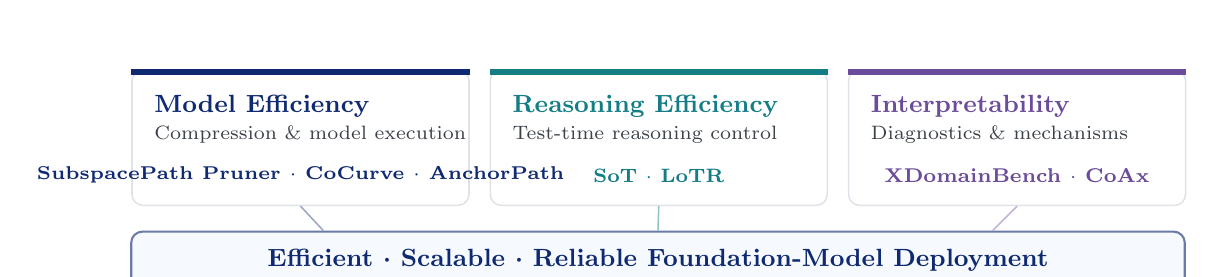
\begin{tikzpicture}[font=\sffamily,x=1cm,y=1cm]
\tikzset{
  domainbox/.style={rounded corners=4pt,draw=MidGray!95,fill=white,line width=.55pt,inner sep=0pt},
  tag/.style={rounded corners=2pt,draw=MidGray!95,fill=SoftGray!80,line width=.32pt,
    inner xsep=3.8pt,inner ysep=2.0pt,font=\scriptsize\bfseries},
  objective/.style={rounded corners=4pt,draw=NTUblue!62,fill=SoftBlue!55,line width=.75pt,
    minimum height=.73cm,align=center,font=\small\bfseries,text=NTUblue}
}
% Three complementary domains. Panels deliberately do not overlap: the diagram shows
% complementarity and contribution to a shared objective, not strict set intersections.
\node[domainbox,minimum width=4.28cm,minimum height=1.72cm,anchor=north west] (d1) at (0,0) {};
\node[domainbox,minimum width=4.28cm,minimum height=1.72cm,anchor=north west] (d2) at (4.55,0) {};
\node[domainbox,minimum width=4.28cm,minimum height=1.72cm,anchor=north west] (d3) at (9.10,0) {};
\fill[NTUblue] (d1.north west) rectangle ([yshift=-.08cm]d1.north east);
\fill[Teal] (d2.north west) rectangle ([yshift=-.08cm]d2.north east);
\fill[Purple] (d3.north west) rectangle ([yshift=-.08cm]d3.north east);

\node[anchor=north west,text=NTUblue,font=\bfseries\small] at ([xshift=.17cm,yshift=-.21cm]d1.north west) {Model Efficiency};
\node[anchor=north west,text=Teal,font=\bfseries\small] at ([xshift=.17cm,yshift=-.21cm]d2.north west) {Reasoning Efficiency};
\node[anchor=north west,text=Purple,font=\bfseries\small] at ([xshift=.17cm,yshift=-.21cm]d3.north west) {Interpretability};

\node[anchor=north west,text=DarkGray,font=\scriptsize] at ([xshift=.17cm,yshift=-.60cm]d1.north west) {Compression \& model execution};
\node[anchor=north west,text=DarkGray,font=\scriptsize] at ([xshift=.17cm,yshift=-.60cm]d2.north west) {Test-time reasoning control};
\node[anchor=north west,text=DarkGray,font=\scriptsize] at ([xshift=.17cm,yshift=-.60cm]d3.north west) {Diagnostics \& mechanisms};

% Project labels: compact text rather than individual chips, to avoid truncation
% while keeping each domain visually readable at report scale.
\node[anchor=south,text=NTUblue,font=\fontsize{6.7}{7.4}\selectfont\bfseries,align=center]
  at ([yshift=.17cm]d1.south) {SubspacePath Pruner $\cdot$ CoCurve $\cdot$ AnchorPath};
\node[anchor=south,text=Teal,font=\scriptsize\bfseries,align=center]
  at ([yshift=.17cm]d2.south) {SoT $\cdot$ LoTR};
\node[anchor=south,text=Purple,font=\fontsize{7.2}{8}\selectfont\bfseries,align=center]
  at ([yshift=.17cm]d3.south) {XDomainBench $\cdot$ CoAx};

\node[objective,minimum width=13.38cm,anchor=north] (obj) at (6.69,-2.05)
  {Efficient $\boldsymbol\cdot$ Scalable $\boldsymbol\cdot$ Reliable Foundation-Model Deployment};
\draw[NTUblue!42,line width=.55pt] (d1.south) -- ([xshift=-4.25cm]obj.north);
\draw[Teal!48,line width=.55pt] (d2.south) -- (obj.north);
\draw[Purple!42,line width=.55pt] (d3.south) -- ([xshift=4.25cm]obj.north);
\end{tikzpicture}
}
\caption{Research landscape. Three complementary research domains contribute to one deployment objective; project labels indicate their primary placement.}
\label{fig:research-topics}
\end{figure}

\begin{thesisbox}
\textbf{Core question.} How can foundation models achieve \textbf{efficient, scalable, and reliable deployment} under heterogeneous scenarios and reasoning demands, and how can their internal structure provide useful evidence for deciding when and how to adapt?
\end{thesisbox}

The research framework has two technical parts, summarized project-by-project in Figure~\ref{fig:qe_overview}:
\begin{itemize}[leftmargin=1.30em,itemsep=0.08em,topsep=0.04em]
  \item \textbf{Part I -- Adaptive Model Execution} studies how a pretrained backbone can be specialized and compressed for heterogeneous deployment scenarios, from scenario-conditioned execution to interaction-aware and high-sparsity structured compression.
  \item \textbf{Part II -- Adaptive Reasoning} studies how test-time reasoning can adapt to heterogeneous problems, first by controlling the reasoning trajectory from the model's evolving state and then by controlling the internal pathway that executes each reasoning step.
\end{itemize}

Figure~\ref{fig:qe_overview} then shows how the two technical parts unfold project by project.
\begin{figure}[H]
\centering
\resizebox{0.86\textwidth}{!}{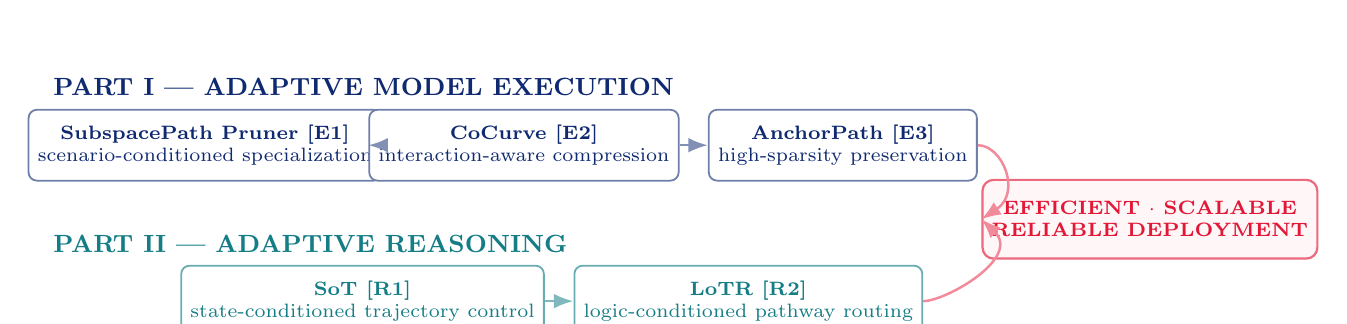
\begin{tikzpicture}[x=1cm,y=1cm,font=\sffamily,>=Latex]
  \tikzset{
    work/.style={rounded corners=3pt,minimum width=3.05cm,minimum height=.90cm,
      align=center,line width=.65pt,font=\bfseries\scriptsize,fill=white},
    goal/.style={rounded corners=4pt,minimum width=3.45cm,minimum height=1.00cm,
      align=center,line width=.8pt,font=\bfseries\scriptsize,fill=NTUred!4,text=NTUred,draw=NTUred!65}
  }
  \node[font=\bfseries\small,text=NTUblue,anchor=west] at (0,1.62) {PART I --- ADAPTIVE MODEL EXECUTION};
  \node[work,draw=NTUblue!60,text=NTUblue] (sp) at (2.05,.88)
    {SubspacePath Pruner [E1]\\\normalfont scenario-conditioned specialization};
  \node[work,draw=NTUblue!60,text=NTUblue] (cc) at (6.10,.88)
    {CoCurve [E2]\\\normalfont interaction-aware compression};
  \node[work,draw=NTUblue!60,text=NTUblue] (ap) at (10.15,.88)
    {AnchorPath [E3]\\\normalfont high-sparsity preservation};
  \draw[->,NTUblue!52,line width=.9pt] (sp.east) -- (cc.west);
  \draw[->,NTUblue!52,line width=.9pt] (cc.east) -- (ap.west);

  \node[font=\bfseries\small,text=Teal,anchor=west] at (0,-.38) {PART II --- ADAPTIVE REASONING};
  \node[work,draw=Teal!64,text=Teal] (sot) at (4.05,-1.10)
    {SoT [R1]\\\normalfont state-conditioned trajectory control};
  \node[work,draw=Teal!64,text=Teal] (lotr) at (8.95,-1.10)
    {LoTR [R2]\\\normalfont logic-conditioned pathway routing};
  \draw[->,Teal!54,line width=.9pt] (sot.east) -- (lotr.west);

  \node[goal] (goal) at (14.05,-.06)
    {EFFICIENT $\cdot$ SCALABLE\\RELIABLE DEPLOYMENT};
  \draw[->,NTUred!50,line width=.9pt] (ap.east) .. controls (12.18,.88) and (12.42,.28) .. (goal.west);
  \draw[->,NTUred!50,line width=.9pt] (lotr.east) .. controls (11.46,-1.10) and (12.42,-.55) .. (goal.west);
\end{tikzpicture}
}
\caption{Research roadmap. The two technical lines progress from deployment conditions to adaptive decisions and converge on efficient, scalable, and reliable foundation-model deployment.}
\label{fig:qe_overview}
\end{figure}

The programme is motivated by two complementary observations. At the behavioral level, heterogeneous and compositional reasoning can expose failures even in models that appear capable on the constituent knowledge involved. At the mechanistic level, model internals exhibit structured redundancy, coupling, compensation, and self-repair, suggesting that internal evidence can be used not only to explain model behavior but also to guide more effective deployment decisions~\citep{gong2026xdomainbench,gong2026coax}. These observations establish the background for the two technical parts rather than forming a separate research branch.

The projects then develop a consistent progression. In \textbf{Part I}, \SubspacePath{}\workref{E1}{sec:subspace} first couples deployment context to a scenario-specific executable pathway without scenario-specific training; \CoCurve{}\workref{E2}{sec:cocurve} broadens the problem to model-wide structured compression by accounting for interactions among units; \AnchorPath{}\workref{E3}{sec:anchor} further extends the usable compression range by preserving quality at higher pruning ratios. In \textbf{Part II}, \SoT{}\workref{R1}{sec:sot} turns reasoning into a state-conditioned closed loop over evidence and stopping, while \LoTR{}\workref{R2}{sec:lotr} keeps existing reasoning paradigms intact and improves them from inside the backbone through logic-conditioned pathway routing. Across the five technical projects, the recurring strategy is to \emph{read the current operating condition, identify the computation it actually needs, and allocate model or reasoning resources accordingly}~\citep{gong2026subspacepath,gong2026cocurve,gong2026anchorpath,gong2026sot,gong2026lotr}.

\begin{thesisbox}
\textbf{Programme-level outcome.} Taken together, the studies expand the quality--efficiency frontier in both model execution and reasoning while testing the mechanisms that make adaptation reliable. The result is a unified PhD programme: \textbf{reduce unnecessary computation, preserve the capability needed by the current condition, and use model-derived evidence to decide when adaptation is trustworthy.}
\end{thesisbox}

{\footnotesize\textbf{Project links:} \XDB{}\projecticon{https://gongzhiren.github.io/XDomainBench-website/}\; \CoAx{}\projecticon{https://gongzhiren.github.io/Conditional-Co-Ablation-website/}\; \SubspacePath{}\projecticon{https://gongzhiren.github.io/SubspacePathPruner-website/}\; \CoCurve{}\projecticon{https://gongzhiren.github.io/CoCurve-website/}\; \AnchorPath{}\projecticon{https://gongzhiren.github.io/AnchorPath-website/}\; \SoT{}\projecticon{https://gongzhiren.github.io/SoT-website/}\; \LoTR{}\projecticon{https://gongzhiren.github.io/LoTR-website/}}
\endgroup
\clearpage
\begingroup\small\singlespacing\setcounter{tocdepth}{2}\tableofcontents\endgroup
\clearpage
\begingroup\footnotesize\singlespacing
\listoffigures
\vspace{2mm}
\listoftables
\endgroup
\clearpage
\pagenumbering{arabic}

% ======================================================================
\section{Introduction}
\label{sec:intro}

\subsection{From capability to deployment}

Foundation models now support a broad range of language, coding, scientific, and multimodal tasks. As the same pretrained backbones are deployed across more environments, a new set of questions becomes central: how much of the model should be executed for a given scenario, how should reasoning effort change with the problem at hand, and how can these decisions remain reliable when the model's internal computation is highly coupled? In practice, a strong model is useful only if its capability can be delivered under realistic memory, latency, data, and reliability constraints.

Three constraints recur throughout this report and are summarized in Table~\ref{tab:mismatches}. \textbf{(1) Heavy model backbones} make full execution expensive in memory, latency, and serving cost, while collecting labels and retraining a specialized model for every scenario is rarely practical. \textbf{(2) Heterogeneous test-time demand} changes what reasoning is useful from problem to problem and from step to step: some cases need broad evidence, some need verification, and some should terminate early. \textbf{(3) Complex internal mechanisms} make selective deployment harder to design and validate because redundancy, cross-module coupling, and compensatory computation can make a local decision depend on the rest of the model.

\begin{table}[H]
\centering\singlespacing\small
\caption{Three deployment constraints and the corresponding research direction.}
\label{tab:mismatches}
\renewcommand{\arraystretch}{1.16}
\begin{tabularx}{\textwidth}{@{}p{0.19\textwidth} p{0.31\textwidth} X@{}}
\toprule
\textbf{Constraint} & \textbf{Deployment consequence} & \textbf{Research direction} \\
\midrule
\textbf{Heavy backbone} &
\bulletcell{\item high memory / latency cost \item per-scenario retraining does not scale} &
Specialize or compress the pretrained backbone for the current deployment condition while preserving useful capability. \\
\textbf{Heterogeneous test-time demand} &
\bulletcell{\item reasoning needs differ across tasks \item useful effort changes within a trajectory} &
Adapt evidence, reasoning depth, and execution to the current problem and model state. \\
\textbf{Complex internal mechanisms} &
\bulletcell{\item local changes can have non-local effects \item coupling and compensation complicate prediction} &
Use behavioral and mechanistic evidence to understand model organization and support reliable adaptation. \\
\bottomrule
\end{tabularx}
\end{table}

These constraints lead to the core question of the thesis:
\begin{thesisbox}
\textbf{How can foundation models achieve efficient, scalable, and reliable deployment under heterogeneous scenarios and reasoning demands, and how can model-internal evidence reveal when and how adaptation should be performed?}
\end{thesisbox}

The answer developed in this report is organized around the two technical directions stated in the title: \textbf{Adaptive Model Execution} and \textbf{Adaptive Reasoning}. The first changes how much and which structural computation the backbone executes; the second changes how reasoning unfolds after deployment.

\subsection{Research architecture and questions}

\textbf{Part I -- Adaptive Model Execution} follows a concrete deployment progression. \textbf{First}, \SubspacePath{} specializes one frozen backbone to heterogeneous scenarios when scenario-specific labels and retraining budgets are unavailable. \textbf{Second}, \CoCurve{} moves from scenario-specific head selection to model-wide structured compression, using interactions among attention and FFN units to identify redundancy that independent scores miss. \textbf{Third}, \AnchorPath{} pushes the viable pruning range further by updating the selection signal as previous removals change the remaining model. The three projects therefore move from \emph{scenario specialization}, to \emph{model-wide interaction-aware compression}, to \emph{quality preservation at high structured sparsity}.

\textbf{Part II -- Adaptive Reasoning} addresses heterogeneity after the model is deployed. \textbf{First}, \SoT{} lets the model's evolving state control which historical evidence remains useful and when further reasoning should stop, improving the quality--token--latency trade-off across diverse reasoning tasks. \textbf{Second}, \LoTR{} keeps the outer reasoning paradigm unchanged and improves its internal execution by routing each reasoning step through a pathway matched to the current logic state. This moves from adapting \emph{the reasoning trajectory} to adapting \emph{the internal computation that executes each step}.

Table~\ref{tab:rqs} makes the mapping from the two research questions to the technical progression explicit.
\begin{table}[H]
\centering\singlespacing\small
\caption{Research questions and the technical progression used to answer them.}
\label{tab:rqs}
\renewcommand{\arraystretch}{1.14}
\begin{tabularx}{\textwidth}{@{}p{0.08\textwidth} p{0.42\textwidth} X@{}}
\toprule
& \textbf{Research question} & \textbf{Technical progression} \\
\midrule
\textbf{RQ1} &
How can a pretrained backbone adapt its \textbf{executed capacity} to heterogeneous deployment scenarios under limited data and compute? &
\bulletcell{\item \SubspacePath{}: scenario-conditioned specialization
\item \CoCurve{}: interaction-aware model-wide compression
\item \AnchorPath{}: high-sparsity quality preservation} \\
\textbf{RQ2} &
How can test-time reasoning adapt to \textbf{heterogeneous problems and evolving reasoning states}? &
\bulletcell{\item \SoT{}: endogenous evidence and stopping control
\item \LoTR{}: logic-conditioned internal pathway routing} \\
\bottomrule
\end{tabularx}
\end{table}

The mechanism and diagnostic studies in Section~\ref{sec:diagnostic} complete the research loop around these two questions. They first establish that capable models can still fail under heterogeneous composition, then show that internal computation can reorganize after intervention. These observations explain both \emph{why} adaptive execution and reasoning are needed and \emph{what kind of evidence} can support them. Together, the behavioral diagnosis, mechanistic analysis, and two technical directions form a closed research programme from \textbf{observed deployment difficulty} to \textbf{internal explanation} to \textbf{adaptive intervention}.

\subsection{Scope and evaluation philosophy}

The projects operate on different technical objects, but the report evaluates them with a common set of deployment criteria; Table~\ref{tab:scope-map} shows how each study instantiates this common scope.
\begin{itemize}[leftmargin=1.35em,itemsep=0.08em]
  \item \textbf{Generalization.} Control signals are tested across scenarios, datasets, model families, modalities, or outer reasoning paradigms rather than only in one development setting.
  \item \textbf{Realized efficiency.} Structural or reasoning savings are tied, where applicable, to measured latency, memory, generated tokens, and physically executed or sliced structure rather than nominal masks or FLOPs alone.
  \item \textbf{Mechanistic evidence.} Ablations, interaction measurements, state analyses, and interventions test whether an adaptive decision corresponds to a real functional change.
  \item \textbf{Theory and formal support.} The main methods include theoretical or formal results that characterize the estimator, objective, controller, or operating regime and close the method--evidence loop.
\end{itemize}

\begin{table}[H]
\centering\singlespacing\scriptsize
\caption{How the projects instantiate the common evaluation scope. A check mark indicates a primary source of evidence in the corresponding study.}
\label{tab:scope-map}
\setlength{\tabcolsep}{3.2pt}
\begin{tabularx}{\textwidth}{@{}p{2.9cm} c c c c X@{}}
\toprule
\textbf{Project} & \textbf{Gen.} & \textbf{Real eff.} & \textbf{Mechanism} & \textbf{Theory/formal} & \textbf{Main scope} \\
\midrule
\XDB{} & $\checkmark$ & -- & $\checkmark$ & $\checkmark$ & controlled behavioral diagnosis across composition orders and model families \\
\CoAx{} & $\checkmark$ & -- & $\checkmark$ & $\checkmark$ & intervention-conditioned circuit importance and causal repair \\
\SubspacePath{} & $\checkmark$ & $\checkmark$ & $\checkmark$ & $\checkmark$ & scenario specialization, transfer, and physical pruning efficiency \\
\CoCurve{} & $\checkmark$ & $\checkmark$ & $\checkmark$ & $\checkmark$ & interaction-aware structured pruning across LLMs and VLMs \\
\AnchorPath{} & $\checkmark$ & $\checkmark$ & $\checkmark$ & $\checkmark$ & quality preservation as structured sparsity increases \\
\SoT{} & $\checkmark$ & $\checkmark$ & $\checkmark$ & $\checkmark$ & quality--token--latency trade-offs across reasoning regimes \\
\LoTR{} & $\checkmark$ & $\checkmark$ & $\checkmark$ & $\checkmark$ & transfer across outer paradigms, backbones, and internal routes \\
\bottomrule
\end{tabularx}
\end{table}

\begin{evidencebox}
\textbf{Notation conventions.} Throughout the report, $(\ell,h)$ indexes attention head $h$ in layer $\ell$, $\mathcal H$ denotes a head inventory, $z$ denotes model logits, and $t$ indexes a reasoning or iterative step. The structured removal ratio is denoted by $\rho$. Project-specific variables are introduced locally at first use; in particular, $q$ denotes a scenario mixture in \SubspacePath{}, $m_t$ an endogenous reasoning state in \SoT{}, and $\mathcal D_k$ the set removed after pruning stage $k$ in \AnchorPath{}. In \LoTR{}, $\pi_t^{(\ell)}$ denotes the predicted logic-state mixture, $T_k^{(\ell,h)}$ a cached state-specific head template, and $J_{\ell,h,k}$ the logic-state--head coupling. This avoids reusing one state symbol for unrelated objects across projects.
\end{evidencebox}

\clearpage
% ======================================================================
\section{Background and Literature Review}
\label{sec:lit}

This thesis intersects three mature research areas, but it approaches them from one deployment question: how can a capable pretrained model adapt its use of capacity and reasoning when the operating condition changes? This section first introduces the purpose of each area, then identifies the specific deployment gap addressed by the projects in this report.

\subsection{Model compression and efficient execution}
Model compression aims to reduce the resource cost of neural networks while preserving useful capability. For foundation models, structured pruning is especially relevant to deployment because removing attention heads, FFN channels, layers, or other hardware-realizable units can produce a physically smaller model with lower memory and inference cost. Prior work established strong non-uniformity in head importance~\citep{michel2019sixteen,voita2019heads} and developed gradient-, activation-, reconstruction-, or loss-based criteria for structured LLM pruning~\citep{ma2023llmpruner,an2024flap,ashkboos2024slicegpt}. Classical second-order pruning further motivates curvature-aware criteria when first-order importance is insufficient~\citep{lecun1989obd,hassibi1993obs}.

\textbf{Scenario-specific deployment.} A practical model may serve many coherent domains or workflows, yet most pruning methods produce one global subnetwork. Re-pruning or retraining for every new scenario adds data and optimization cost, and a global ranking can be brittle under domain shift. \SubspacePath{} addresses this deployment setting by learning a reusable representation--parameter coupling offline and compiling a scenario-specific head pathway online from input-only signals~\citep{gong2026subspacepath}.

\textbf{Interaction-aware structured compression.} Even with a well-defined deployment condition, deleting a \emph{set} of Transformer units is not generally equivalent to summing their independent effects. Attention and FFN blocks communicate through the same residual stream, so removal decisions can reinforce or cancel one another. \CoCurve{} therefore moves from scalar node scores to an output-grounded interaction matrix and jointly allocates a shared structured budget across modules~\citep{gong2026cocurve}.

\textbf{High-sparsity compression.} At higher pruning ratios, the challenge changes again: a criterion calibrated at the dense model is extrapolated farther from the point where it was estimated. \AnchorPath{} studies this regime directly and reframes pruning as an anchored continuation problem, repeatedly updating the local selection signal while retaining a fixed dense reference~\citep{gong2026anchorpath}. This extends the model-execution line from \emph{what to remove} to \emph{how to maintain a trustworthy selection process as compression becomes more aggressive}.

\subsection{Reasoning and test-time computation}
Test-time reasoning research asks how a frozen or lightly adapted model can use additional inference-time computation to solve difficult problems. Chain-of-thought, planning, iterative revision, self-consistency, search, and related methods improve reasoning by imposing richer external procedures or allocating more samples and steps~\citep{wei2022chain,wang2023plan,madaan2023self,wang2023selfconsistency,yao2023tree,snell2025scaling,brown2024large}. Memory and context-compression methods reduce the cost of maintaining long histories~\citep{li2023compressing,jiang2024longllmlingua}. These results establish that inference organization can be as important as the frozen backbone.

\textbf{Adaptive reasoning across heterogeneous problems.} A fixed reasoning recipe is unlikely to be optimal for every task or every stage of a trajectory: easy problems can waste tokens, while difficult steps may need more evidence or verification. \SoT{} treats this mismatch as a feedback-control problem. It reads a compact endogenous reasoning state and lets that state choose historical evidence and stopping, so reasoning depth and context are adapted rather than prescribed in advance~\citep{gong2026sot}.

\textbf{Improving existing paradigms from inside the model.} Stronger outer procedures still leave the internal pathway of each reasoning step largely unmanaged. \LoTR{} therefore keeps the external paradigm unchanged and introduces a plug-in internal controller: recurring logic states are inferred from intermediate readouts and coupled to reusable head-pathway templates~\citep{gong2026lotr}. This separates two control layers that are often conflated---\emph{which reasoning algorithm is run} and \emph{how the backbone executes each step of that algorithm}.

\subsection{Interpretability, diagnostics, and mechanism}
Interpretability provides tools for asking what information a model represents and which internal computations causally support a behavior. Linear probing and representation engineering expose readable semantic structure in intermediate states~\citep{alain2016understanding,belinkov2022probing,zou2023representationengineering}; mechanistic interpretability uses attribution and intervention to localize causal circuits~\citep{elhage2021framework,wang2022ioi,conmy2023acdc,kramar2024atp}. Work on self-repair further shows that interventions can recruit compensatory computation~\citep{mcgrath2023hydra,rushing2024selfrepair}. For this thesis, interpretability is not a separate endpoint: it provides \emph{diagnostic evidence and internal signals} that help explain when adaptive deployment is necessary and how it might be controlled.

\textbf{Behavioral diagnosis under heterogeneous composition.} Aggregate benchmark accuracy can hide whether a model lacks constituent knowledge or fails when familiar knowledge must be composed. \XDB{} constructs controllable multi-domain, multi-turn scientific reasoning settings so that composition difficulty and trajectory degradation can be studied separately~\citep{gong2026xdomainbench}. The resulting failure pattern motivates the need for deployment-aware execution and reasoning rather than assuming that capability measured in isolation will transfer unchanged.

\textbf{Mechanistic importance under intervention.} Standard component scores are usually measured in the intact model, but an intervention can change which computation becomes necessary. \CoAx{} uses self-repair as a concrete case: it compares a component's finite effect before and after a supplied primary circuit is removed, recovering dormant backup computation that is invisible to intact-state scoring~\citep{gong2026coax}. This supplies a mechanistic reason to treat internal importance as conditional and later motivates interaction-aware compression.

\subsection{Research positioning}
The three literatures therefore contribute complementary pieces of the same programme. Model compression addresses the cost of the backbone; test-time reasoning addresses the cost and organization of inference; interpretability and diagnostics explain the failure modes and internal structure that make adaptation necessary. Table~\ref{tab:gapmap} summarizes the gap addressed in each area and the corresponding response developed in this report.

\begin{table}[H]
\centering\singlespacing\footnotesize
\caption{Positioning of the research programme across three literatures.}
\label{tab:gapmap}
\renewcommand{\arraystretch}{1.16}
\setlength{\tabcolsep}{4.2pt}
\begin{tabularx}{\textwidth}{@{}p{3.0cm} p{5.1cm} X@{}}
\toprule
\textbf{Area} & \textbf{Deployment gap} & \textbf{Research response} \\
\midrule
\textbf{Model compression / execution} &
\bulletcell{\item global subnetworks are brittle across scenarios
\item unitwise scores miss interactions
\item dense-point criteria weaken at high sparsity} &
\bulletcell{\item scenario-conditioned specialization
\item interaction-aware structured compression
\item refreshed selection at high sparsity} \\
\textbf{Reasoning / test-time computation} &
\bulletcell{\item fixed procedures misallocate test-time compute
\item outer paradigms leave internal execution unmanaged} &
\bulletcell{\item state-conditioned evidence and stopping
\item logic-conditioned internal routing} \\
\textbf{Interpretability / diagnostics} &
\bulletcell{\item aggregate accuracy hides composition failure
\item intact-state attribution can miss repair} &
\bulletcell{\item controlled behavioral diagnosis
\item intervention-conditioned mechanism analysis} \\
\bottomrule
\end{tabularx}
\end{table}

This positioning is intentionally selective. The thesis does not attempt to unify compression, reasoning, and interpretability as research fields; it uses each field to answer a different part of a single deployment problem, with the projects connected by a common emphasis on condition-aware decisions and model-derived evidence.

\clearpage
% ======================================================================
\section{Background Observations: External Demand and Internal Mechanism}
\label{sec:diagnostic}

Before the two technical parts, I use two studies to make the deployment problem concrete from complementary viewpoints. \XDB{}\workref{D1}{sec:xdb} looks outward: what happens when a capable model must reason across heterogeneous, interacting demands? \CoAx{}\workref{D2}{sec:coax} looks inward: what happens to the model's computation when an important pathway is perturbed? The first reveals a gap between isolated capability and realistic composition; the second reveals structured adaptation inside the network. These observations motivate the later execution and reasoning controllers.

\subsection{External observation: heterogeneous reasoning in \XDB{} \texorpdfstring{\projecticon{https://gongzhiren.github.io/XDomainBench-website/}}{}}
\label{sec:xdb}

\textbf{Motivation.} Capable foundation models are increasingly asked to reason across scientific, engineering, and other knowledge-intensive settings in which several domains appear together and the relevant context changes over a multi-turn interaction. This creates a direct deployment question: \emph{can a capable foundation model still reason reliably when the problem becomes heterogeneous and compositional?} \XDB{} was designed as a diagnostic benchmark for this question, rather than as another isolated knowledge test~\citep{gong2026xdomainbench}.

Figure~\ref{fig:xdb-framework} gives the high-level benchmark organization before the empirical observations are discussed.
\begin{figure}[H]
\centering
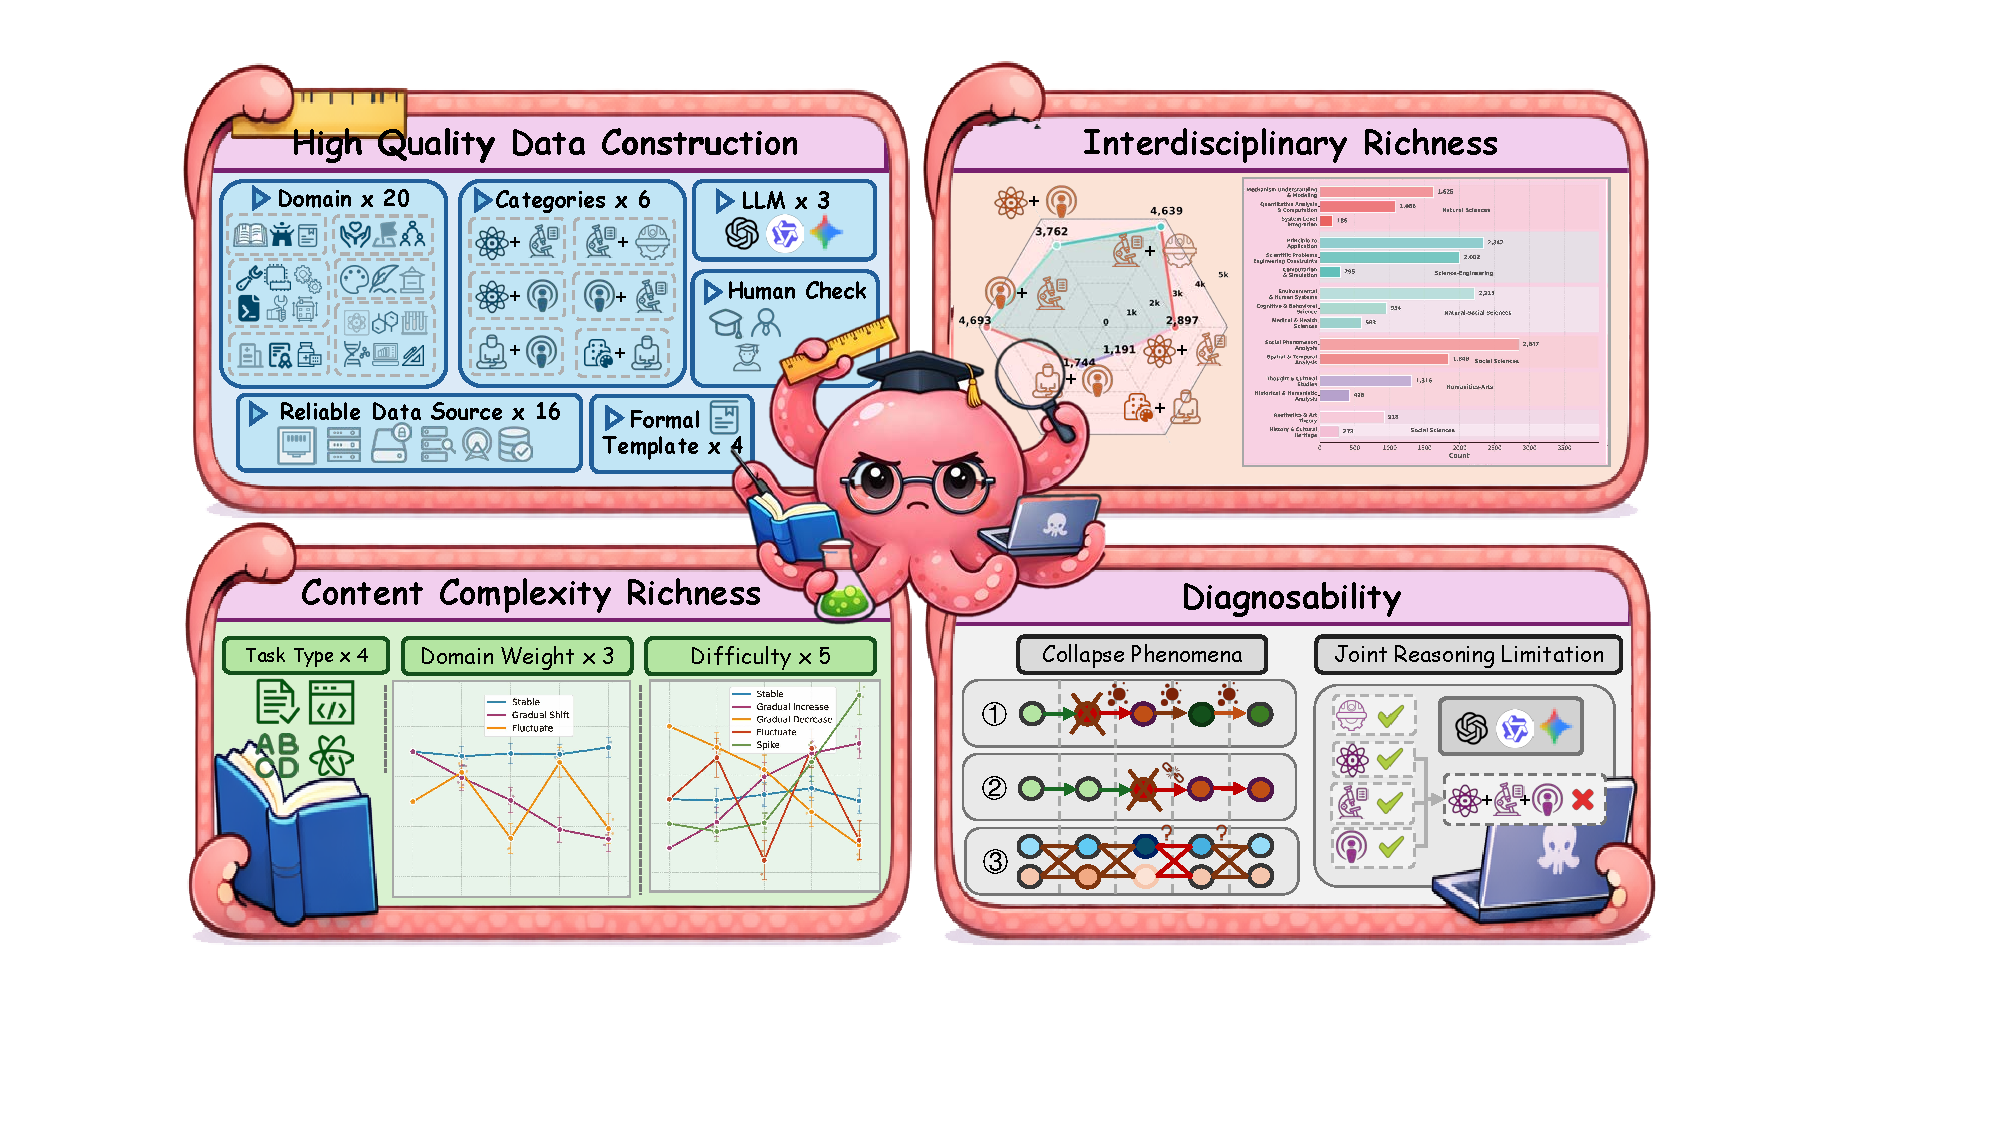
\includegraphics[width=0.94\textwidth]{xdb_framework_source.pdf}
\caption{Overview of the \XDB{} framework. The benchmark organizes interdisciplinary scientific problems into controlled interactive sessions, allowing heterogeneous composition and multi-turn degradation to be studied within the same evaluation.}
\label{fig:xdb-framework}
\end{figure}

\textbf{Benchmark positioning.} Three design properties make the benchmark useful as a deployment stress test. \textbf{First}, composition order is explicit, so the number of scientific domains involved can be increased systematically instead of being hidden inside an aggregate difficulty label. \textbf{Second}, the benchmark is interactive, which separates the immediate burden of combining heterogeneous knowledge from failures that accumulate over later turns. \textbf{Third}, its construction preserves constituent-domain questions and cross-domain combinations, making it possible to distinguish weak isolated knowledge from weak composition of knowledge that the model otherwise handles well.

\begin{figure}[tbp]
\centering
\begin{minipage}[t]{0.54\textwidth}
\centering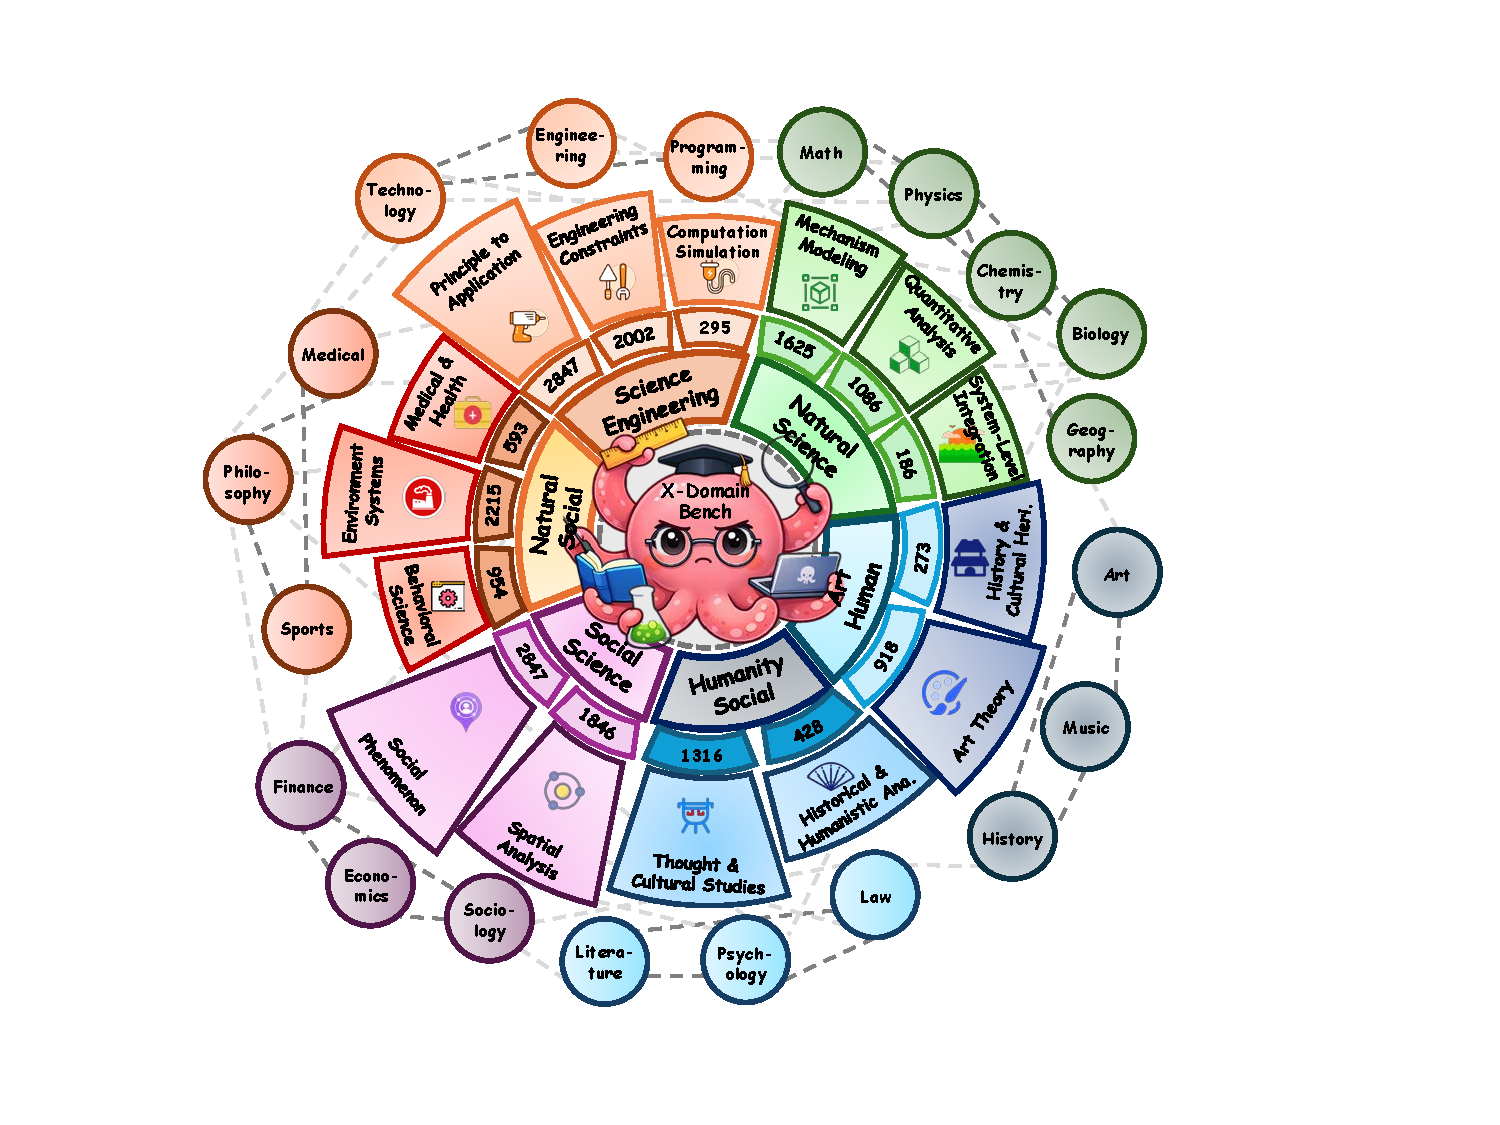
\includegraphics[width=\linewidth]{xdb_taxonomy_source.pdf}
\captionof{figure}{Scientific-domain coverage in \XDB{}. Twenty domains span six broad scientific categories, creating a controlled space for heterogeneous composition.}
\label{fig:xdb-taxonomy}
\end{minipage}\hfill
\begin{minipage}[t]{0.41\textwidth}
\centering
\captionof{table}{Scale of \XDB{}.\label{tab:xdb-scale}}
\singlespacing\footnotesize
\renewcommand{\arraystretch}{1.10}
\begin{tabular}{@{}lr@{}}
\toprule
\textbf{Dimension} & \textbf{Scale}\\
\midrule
Scientific domains & 20\\
Scientific categories & 6\\
Cross-domain combinations & 62\\
Interdisciplinary themes & 15\\
Interactive sessions & 8,598\\
Total turns & 52,582\\
Task categories & 4\\
Composition order & $k=1\!\rightarrow\!4$\\
\bottomrule
\end{tabular}
\end{minipage}
\end{figure}

Figure~\ref{fig:xdb-taxonomy} and Table~\ref{tab:xdb-scale} summarize the breadth and scale of the benchmark. The scale matters because the central phenomenon is not tied to a single domain pair or a single model. Table~\ref{tab:xdb-overall} reproduces the benchmark-wide scaling view: across large dense models, smaller dense models, and MoE models, increasing composition order changes both turn-level quality and session-level success.

\begin{table}[tbp]
\centering\singlespacing\tiny
\caption{Overall \XDB{} scaling results as composition order increases ($k=1\rightarrow4$). Left: deterministic problems; right: open-world problems. R = Recall, F1 = F1-score, and S@t = SessionSuccess@$\tau$. Values follow the normalized benchmark evaluation reported for the benchmark.}
\label{tab:xdb-overall}
\setlength{\tabcolsep}{0.65pt}\renewcommand{\arraystretch}{1.03}
\begin{adjustbox}{max width=\textwidth}
\begin{tabular}{lccc|ccc|ccc|ccc||ccc|ccc|ccc|ccc}
\toprule
 & \multicolumn{12}{c}{\textbf{Deterministic problems}} & \multicolumn{12}{c}{\textbf{Open-world problems}}\\
\cmidrule(lr){2-13}\cmidrule(lr){14-25}
& \multicolumn{3}{c}{$k=1$}&\multicolumn{3}{c}{$k=2$}&\multicolumn{3}{c}{$k=3$}&\multicolumn{3}{c}{$k=4$}
&\multicolumn{3}{c}{$k=1$}&\multicolumn{3}{c}{$k=2$}&\multicolumn{3}{c}{$k=3$}&\multicolumn{3}{c}{$k=4$}\\
\textbf{Model}&R&F1&S@t&R&F1&S@t&R&F1&S@t&R&F1&S@t&R&F1&S@t&R&F1&S@t&R&F1&S@t&R&F1&S@t\\
\midrule
\rowcolor{SoftGray}\multicolumn{25}{c}{\textbf{Large models}}\\
GPT-5.2&30.8&22.0&42.5&25.9&11.4&28.8&22.8&8.2&25.2&18.0&4.8&26.9&25.9&9.3&29.6&21.7&7.0&28.2&28.0&5.8&21.4&13.0&5.8&35.3\\
Claude-4.5 Sonnet&30.4&22.8&48.5&28.6&14.0&31.3&21.0&7.3&26.7&19.3&4.5&24.4&30.2&8.0&40.7&23.4&10.3&21.4&13.5&5.5&21.4&13.3&4.0&14.7\\
Claude-4.5 Haiku&30.6&23.0&41.8&29.7&13.7&31.1&26.9&12.3&30.7&23.0&9.5&37.7&19.4&7.0&40.7&22.4&11.0&21.4&32.6&13.8&23.2&19.1&11.5&35.3\\
Gemini-2.5 Flash&27.1&20.4&36.6&21.4&5.3&24.3&18.4&3.0&25.2&13.8&3.1&21.3&18.8&6.9&33.3&22.1&4.1&34.2&13.5&3.3&21.4&12.4&3.7&34.5\\
Gemini-2.0 Flash&27.2&12.9&26.9&22.4&5.6&25.8&20.7&5.0&24.3&15.0&2.8&20.3&26.8&1.8&22.2&16.2&2.8&24.8&12.6&4.6&16.1&11.9&2.3&15.4\\
Qwen2.5-72B&26.8&17.8&35.8&27.0&12.8&27.3&25.0&11.5&28.2&19.9&8.9&32.3&31.3&8.4&25.9&21.9&11.2&20.5&16.1&10.2&21.4&13.2&10.3&32.4\\
\rowcolor{SoftBlue}\textbf{Mean}&28.8&19.8&38.7&25.8&10.5&28.1&22.5&7.9&26.7&18.2&5.6&27.1&25.4&6.9&32.1&21.3&7.7&25.1&19.4&7.2&20.8&13.8&6.3&27.9\\
\midrule
\rowcolor{SoftGray}\multicolumn{25}{c}{\textbf{Small models}}\\
GPT-5-mini&23.1&12.8&25.2&25.3&14.4&21.3&22.4&2.2&20.0&11.4&1.3&20.0&22.0&2.8&10.0&23.1&3.4&20.0&3.2&3.3&10.0&3.2&3.3&10.0\\
Qwen2.5-14B&27.2&19.1&39.6&25.5&11.3&26.6&23.3&9.1&27.7&18.5&7.6&29.9&18.2&3.9&18.5&27.1&10.4&25.6&28.1&9.3&10.7&11.6&7.5&20.6\\
Qwen2.5-7B&26.4&18.4&31.3&25.8&11.5&26.8&23.3&9.8&28.7&18.9&7.3&28.1&50.2&3.7&18.5&22.6&8.6&23.9&11.1&7.6&8.9&14.5&6.8&17.6\\
Llama-3.1-8B&26.2&18.8&35.8&24.7&11.4&23.8&23.3&9.9&28.2&16.5&8.1&25.1&15.2&4.1&14.8&23.9&9.8&29.9&28.9&10.3&17.9&19.0&7.9&29.4\\
Llama-3.2-3B&26.8&16.3&31.3&24.5&10.5&23.8&23.2&8.7&28.7&20.9&5.5&29.9&19.6&3.4&25.9&22.8&8.9&25.6&47.1&6.9&23.2&14.3&5.1&26.5\\
Gemma-2-2B-IT&27.3&18.6&30.6&26.3&12.1&27.6&20.6&7.4&21.8&18.1&4.3&22.6&18.4&4.6&7.4&20.7&8.5&18.8&45.0&7.4&17.9&9.5&2.8&17.6\\
\rowcolor{SoftBlue}\textbf{Mean}&26.2&17.3&32.3&25.3&11.9&25.0&22.7&7.9&25.9&17.4&5.7&25.9&23.9&3.8&15.9&23.4&8.3&24.0&27.2&7.5&14.8&12.0&5.6&20.3\\
\midrule
\rowcolor{SoftGray}\multicolumn{25}{c}{\textbf{MoE models}}\\
Qwen3-Next-80B&63.8&65.7&89.6&46.3&40.1&51.1&41.7&36.4&52.0&29.5&26.3&34.5&10.8&15.0&40.7&29.8&27.9&28.2&26.3&23.9&46.4&25.7&24.1&41.2\\
Mixtral-8$\times$7B&56.4&22.4&74.6&51.9&18.0&46.4&51.0&18.9&48.5&41.0&19.5&49.4&24.1&21.3&40.7&41.9&25.7&35.9&42.0&25.5&53.6&39.9&23.7&55.9\\
\rowcolor{SoftBlue}\textbf{Mean}&60.1&44.0&82.1&49.1&29.1&48.8&46.4&27.6&50.2&35.2&22.9&42.0&17.5&18.1&40.7&35.9&26.8&32.0&34.1&24.7&50.0&32.8&23.9&48.5\\
\bottomrule
\end{tabular}
\end{adjustbox}
\end{table}

The most informative diagnostic is the first turn. Because long-session drift has not yet accumulated, a performance change at turn one isolates the burden introduced by composition itself. Figure~\ref{fig:xdb-turn1} shows this effect directly.

\begin{figure}[H]
\centering
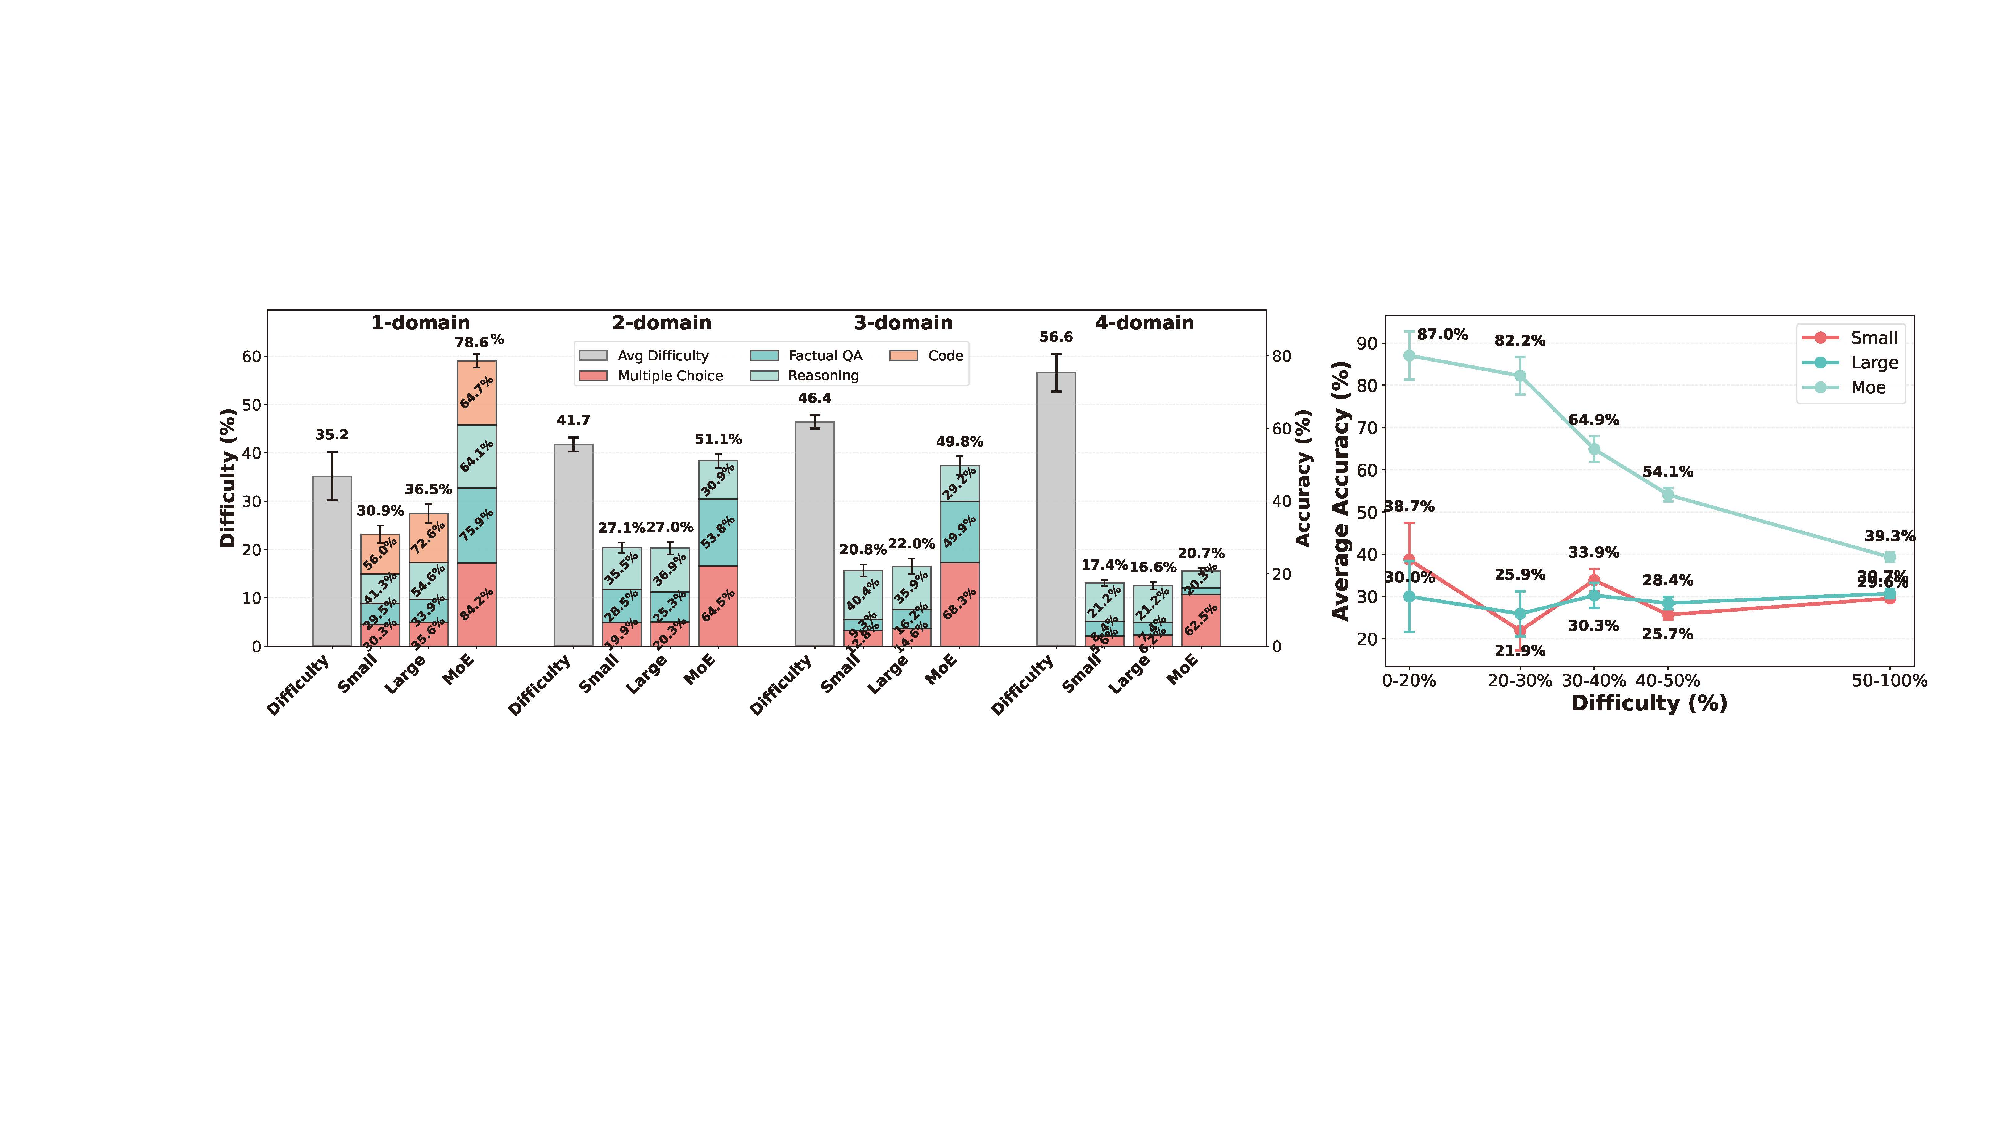
\includegraphics[width=0.90\textwidth]{xdb_turn1_source.pdf}
\caption{First-turn composition effect in \XDB{}. The degradation appears before multi-turn error accumulation, isolating an immediate reasoning burden created by heterogeneous knowledge composition.}
\label{fig:xdb-turn1}
\end{figure}

\textbf{Insight for the thesis.} The important conclusion is not simply that a harder benchmark lowers accuracy. The controlled first-turn result shows that a model can possess useful constituent knowledge yet still lose reliability when that knowledge must be coordinated under a more heterogeneous demand. Multi-turn interaction then amplifies the same weakness through error accumulation, reasoning breaks, and domain confusion. This observation motivates both technical parts of the report: the deployed backbone should avoid executing irrelevant or interfering capacity for the current scenario, and the reasoning process should adapt its evidence and effort to the current problem rather than follow one fixed recipe.

\begin{insightbox}[External observation]
\XDB{} turns heterogeneous deployment from a broad intuition into a controlled behavioral phenomenon: \textbf{capability measured in isolation does not guarantee reliable capability composition}. The rest of the thesis asks how model execution and reasoning can become more responsive to that changing demand.
\end{insightbox}

\subsection{Internal observation: self-repair and conditional importance in \CoAx{} \texorpdfstring{\projecticon{https://gongzhiren.github.io/Conditional-Co-Ablation-website/}}{}}
\label{sec:coax}

\textbf{From failure behavior to internal organization.} The external diagnostic says that the required computation changes. The next question is whether the model's internals themselves expose structure that can support adaptation. \CoAx{} studies self-repair as a clean case where the answer is visible~\citep{gong2026coax}. When a primary circuit is ablated, dormant backup components can increase their contribution and preserve behavior. The lesson for this thesis is broader than circuit discovery: the internal computation of a foundation model is \textbf{conditional, compensatory, and coupled}, so a component cannot always be assigned one fixed intrinsic importance.

The two-state idea is visualized in Figure~\ref{fig:coax}.
\begin{figure}[H]
\centering
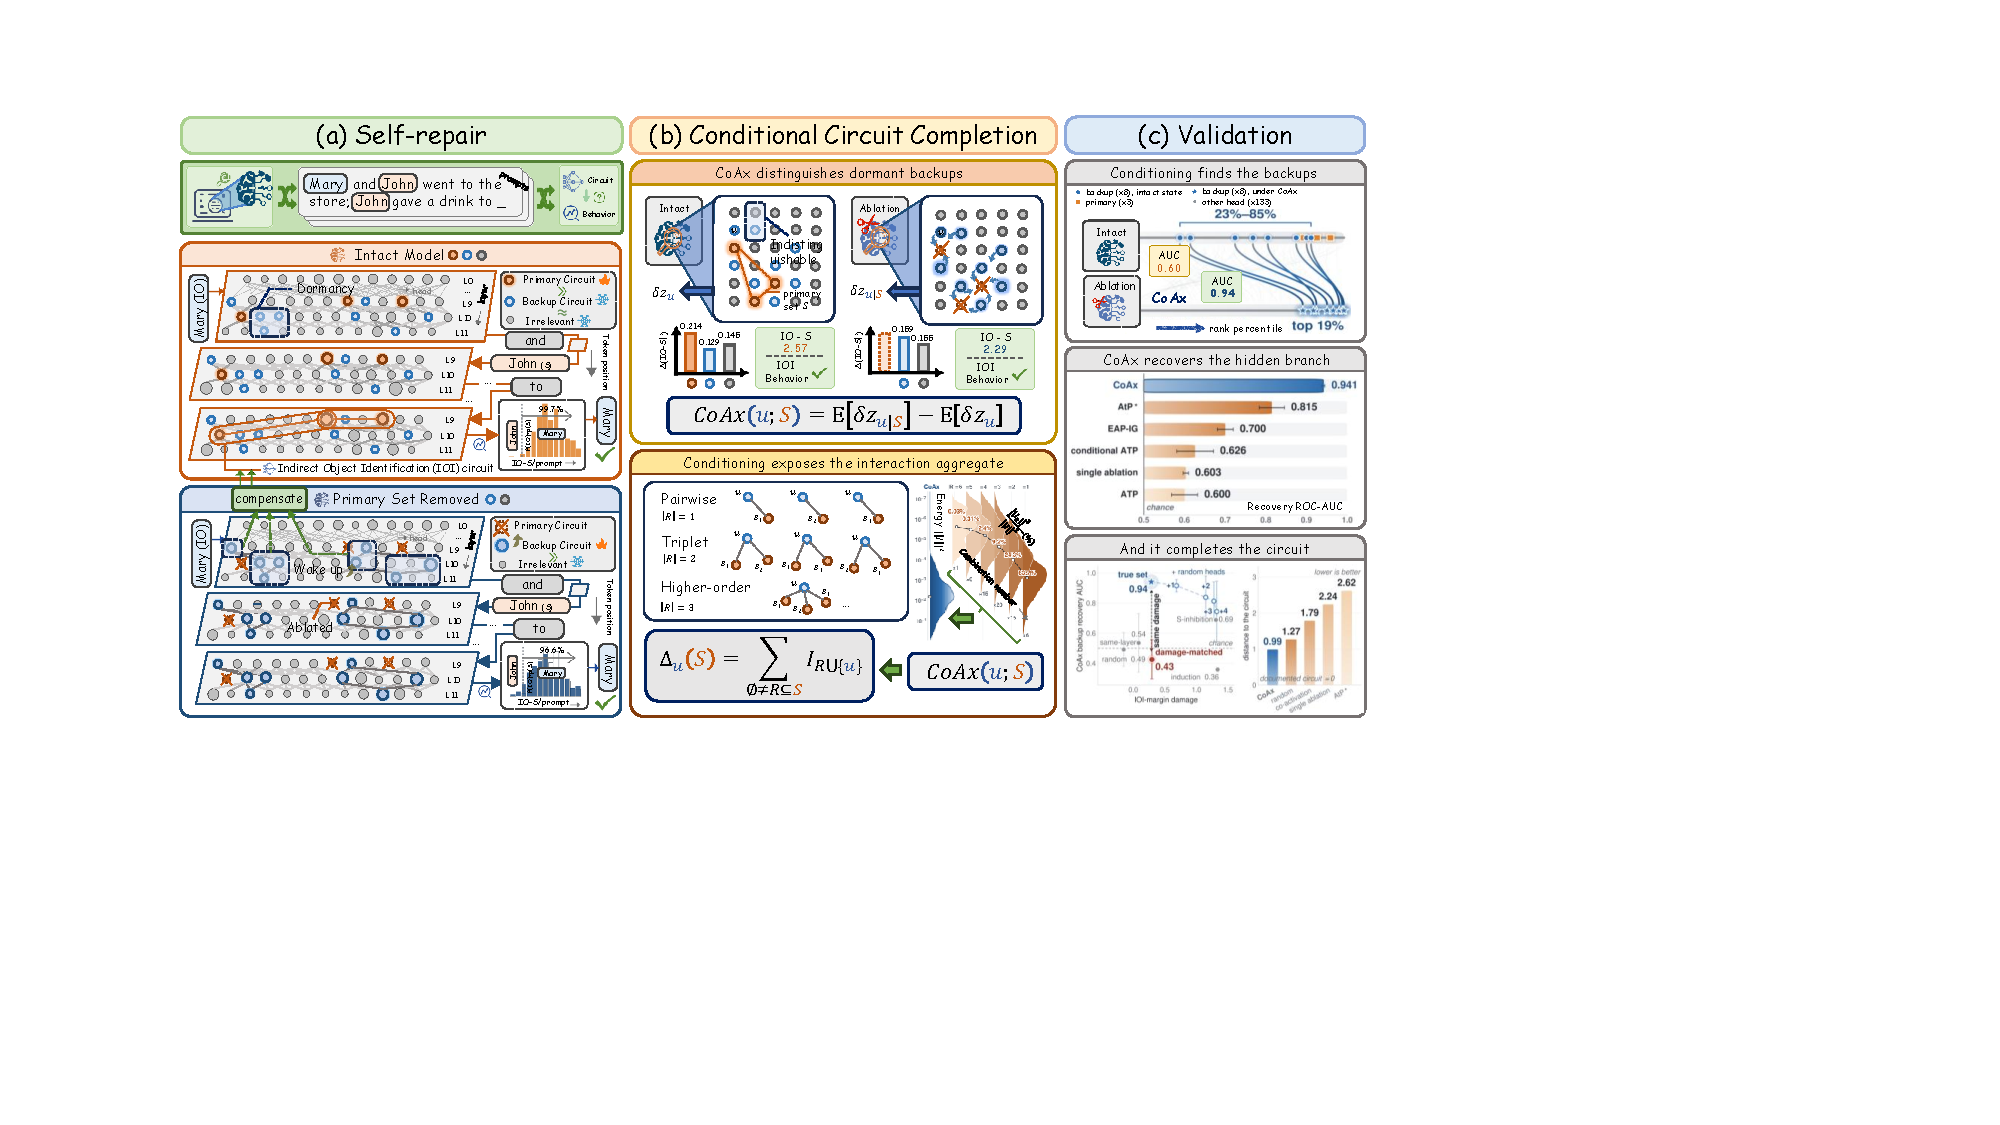
\includegraphics[width=0.91\textwidth]{coax_teaser_full.pdf}
\caption{Conditional circuit completion in \CoAx{}. Removing the primary pathway exposes backup computation that is nearly silent in the intact model but becomes important after intervention.}
\label{fig:coax}
\end{figure}

\subsubsection{Technical core: compare the same component in two model states}
Let $\Sset$ be a supplied primary set and $u$ a candidate component. If ablating a set $M$ produces logits $z_M$, the intact and primary-conditional finite effects are
\begin{equation}
\Delta z_u=z_0-z_{\{u\}},\qquad
\Delta z_{u\mid\Sset}=z_{\Sset}-z_{\Sset\cup\{u\}}.
\label{eq:coax-effects}
\end{equation}
The two effects are measured in a common clean-output Fisher geometry. For perturbation $v$ and $p_0=\operatorname{softmax}(z_0)$,
\begin{equation}
\widetilde v=\sqrt{p_0}\odot\bigl(v-\langle p_0,v\rangle\mathbf 1\bigr),\qquad
\mathcal E(v)=\mathbb E_{x,t}\|\widetilde v\|_2^2.
\label{eq:coax-energy}
\end{equation}
The score is the signed growth of the candidate's effect after the primary set is removed:
\begin{equation}
\operatorname{CoAx}_u(\Sset)=\mathcal E(\Delta z_{u\mid\Sset})-\mathcal E(\Delta z_u).
\label{eq:coax}
\end{equation}
A dormant backup has exactly the desired signature: small effect in the intact model, large effect after $\Sset$ is removed. Subtracting the intact effect distinguishes newly recruited computation from components that were already important before intervention.

The conditional effect also aggregates interactions with the removed set. If $I_T$ denotes the M\"obius interaction for jointly ablating subset $T$,
\begin{equation}
\Delta z_{u\mid\Sset}=\Delta z_u+\sum_{\emptyset\neq R\subseteq\Sset} I_{R\cup\{u\}}.
\label{eq:coax-allorder}
\end{equation}
This provides the mechanistic bridge to later compression work: once importance changes with what else is present, the missing object is a \emph{condition or interaction} that changes the candidate's functional role.

Table~\ref{tab:coax-discovery} shows that the two-state contrast sharply separates the documented backups from intact-only and removed-only scores.
\begin{table}[tbp]
\centering\singlespacing\scriptsize
\caption{Backup-head discovery on GPT-2-small IOI (ROC-AUC over eight documented backups; mean $\pm$ s.d. across four prompt seeds). The three column groups distinguish information available only in the intact model, only after primary removal, and in the two-state contrast.}
\label{tab:coax-discovery}
\setlength{\tabcolsep}{3.0pt}
\begin{tabular}{@{}rrrrrrr@{}}
\toprule
\multicolumn{4}{c}{\textbf{Intact only}} & \multicolumn{2}{c}{\textbf{Removed only}} & \textbf{Intact $\rightarrow$ removed}\\
\cmidrule(lr){1-4}\cmidrule(lr){5-6}\cmidrule(l){7-7}
\makecell{Single\\ablation} & AtP & EAP-IG & \makecell{AtP$^\star$\\GradDrop} & \makecell{Conditional\\gradient} & \makecell{Conditional\\energy} & \textbf{\CoAx{}} \\
\midrule
$0.603\pm0.007$ & $0.600\pm0.032$ & $0.700\pm0.020$ & $0.815\pm0.031$ & $0.626\pm0.045$ & $0.758\pm0.004$ & \textbf{$0.941\pm0.004$} \\
\bottomrule
\end{tabular}
\end{table}

Figure~\ref{fig:coax-handoff} then tests whether the recovered branch actually wakes up and carries the repair.
\begin{figure}[tbp]
\centering
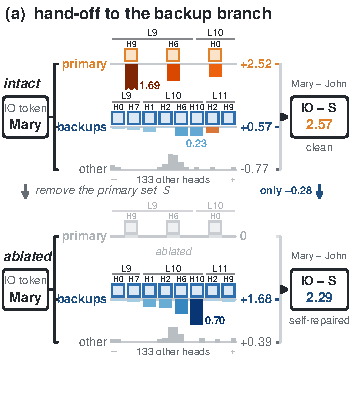
\includegraphics[width=0.43\textwidth]{coax_handoff.pdf}\hfill
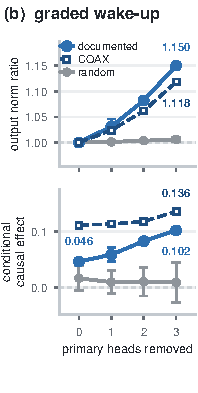
\includegraphics[width=0.24\textwidth]{coax_wakeup.pdf}\hfill
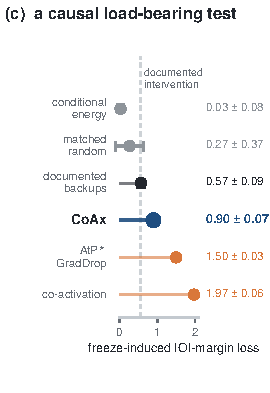
\includegraphics[width=0.29\textwidth]{coax_repair.pdf}
\caption{Backup hand-off and causal repair on GPT-2-small IOI. \textbf{Left:} primary removal shifts direct-logit attribution toward the documented backup branch. \textbf{Middle:} the backup response grows as more primary heads are removed. \textbf{Right:} freezing each selector's top-$8$ at intact-state outputs tests causal load-bearingness; the \CoAx{} selection removes most of the measured repair.}
\label{fig:coax-handoff}
\end{figure}

The hand-off is both graded and causal. Removing the primary name-movers eliminates their direct contribution while the documented backup branch roughly triples its contribution from $+0.57$ to $+1.68$, even as the IO$-$S margin falls only from $2.57$ to $2.29$. Freezing the \CoAx{} top-$8$ at their intact-state outputs causes a $0.90\pm0.07$ point margin loss, compared with $0.03\pm0.08$ for conditional energy alone and $0.27\pm0.37$ for a matched random set. Thus the discovered branch is correlated with the intervention; it carries the repair.

Table~\ref{tab:coax-completion} validates the same branch at circuit level, both by completing an incomplete circuit and by reproducing the documented knockout.
\begin{table}[tbp]
\centering\singlespacing\scriptsize
\caption{Circuit-level validation of the recovered branch. Left: adding the recovered heads to an incomplete primary circuit reduces the counterfactual incompleteness $D(C)$. Right: removing each selector's top-$8$ is compared with the documented backup knockout; lower distances are better.}
\label{tab:coax-completion}
\begin{minipage}[c]{0.36\linewidth}
\centering
\begin{tabular}{@{}lc@{}}
\toprule
\textbf{Circuit} & $\mathbf{D(C)}\downarrow$\\
\midrule
Primary circuit & $0.755\pm0.074$\\
Documented circuit & $0.276\pm0.027$\\
+ \CoAx{} & \textbf{$0.205\pm0.030$}\\
+ random & $0.808\pm0.206$\\
\bottomrule
\end{tabular}
\end{minipage}\hfill
\begin{minipage}[c]{0.61\linewidth}
\centering
\begin{tabular}{@{}lrrr@{}}
\toprule
\textbf{Top-$8$ knockout} & \textbf{Margin dist.}$\downarrow$ & \textbf{Output KL}$\downarrow$ & \textbf{Unrel. KL}$\downarrow$\\
\midrule
Documented backups & 0.00 & 0.00 & 0.09\\
\CoAx{} & \textbf{0.99} & \textbf{0.17} & 0.14\\
Co-activation & 1.79 & 0.47 & 0.15\\
\CoAx{} next-$8$ & 2.24 & 0.64 & 0.54\\
AtP$^\star$ GradDrop & 2.62 & 0.82 & 0.31\\
Random & 1.27 & 0.43 & 0.15\\
\bottomrule
\end{tabular}
\end{minipage}
\end{table}

Figure~\ref{fig:coax-regime} asks whether this conditional signal remains meaningful beyond one circuit and one architecture.
\begin{figure}[tbp]
\centering
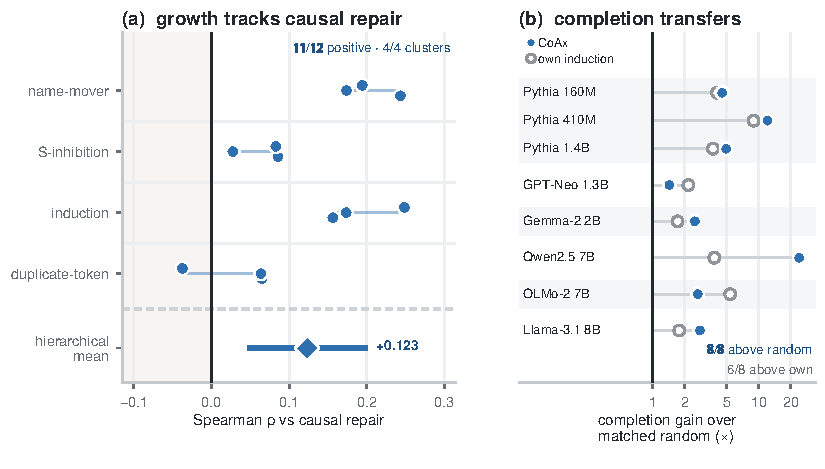
\includegraphics[width=0.88\textwidth]{coax_generalization.pdf}
\caption{Conditional repair generalizes across mechanisms and architectures. Signed conditional growth agrees positively with held-out causal repair in 11/12 instances across four mechanism clusters, while \CoAx{}-based completion beats matched random completion on all eight non-GPT-2 models spanning six architecture families.}
\label{fig:coax-regime}
\end{figure}

The generalization result is important for how this diagnostic is used in the thesis. The phenomenon is not confined to one annotated IOI circuit: the same signed conditional signal tracks held-out repair across distinct mechanisms and supports circuit completion across multiple model families. This makes self-repair a concrete demonstration that foundation-model internals contain structured, reusable information about \emph{how computation reorganizes under change}.

\begin{insightbox}[From diagnosis to research methodology]
\XDB{} establishes the \textbf{external premise}: deployment changes \emph{what capability must be composed}. \CoAx{} establishes the \textbf{internal premise}: intervention can change \emph{which computation carries the behavior}. Together they motivate the methodology used throughout the report: \textbf{(i)} read a compact condition or state without scenario-specific retraining, \textbf{(ii)} connect that signal to an executable allocation decision, and \textbf{(iii)} model interactions explicitly whenever local importance depends on what else is active, removed, or already executed. Part~I applies this principle to structural model execution; Part~II applies it to reasoning-time computation.
\end{insightbox}

\clearpage
% ======================================================================
\section{Part I: Adaptive Model Execution}
\label{sec:execution}

Part~I develops three increasingly demanding forms of adaptive model execution: \textbf{scenario-conditioned specialization} (Section~\ref{sec:subspace}), \textbf{interaction-aware model-wide compression} (Section~\ref{sec:cocurve}), and \textbf{quality preservation at high structured sparsity} (Section~\ref{sec:anchor}). The progression is deliberate: first adapt a frozen backbone to the current scenario, then remove redundancy while accounting for interactions across the full model, and finally preserve that selection quality when the pruning ratio becomes high.

\begin{transitionbox}
\textbf{Part I question.} Can one pretrained foundation model be made substantially cheaper to execute across heterogeneous deployment conditions, while preserving the capacity that remains important for the current scenario and operating regime?
\end{transitionbox}

\subsection{Scenario-Conditioned Model Specialization with \SubspacePath{} \texorpdfstring{\projecticon{https://gongzhiren.github.io/SubspacePathPruner-website/}}{}}
\label{sec:subspace}

\textbf{Deployment problem.} A general-purpose model may be reused across many coherent deployment scenarios---a scientific subfield, an operational assistant, or a repeated domain-specific workflow---but a practical deployment often has \emph{no scenario-specific labels, no retraining budget, and no time to run a new pruning optimization for every incoming scenario}. A single global pruning ranking is equally unsatisfactory because the computation useful in one scenario need not be the computation useful in another. \SubspacePath{} therefore asks whether the scenario can be read from input-only signals and compiled directly into a reusable internal pathway, with all expensive preparation amortized offline~\citep{gong2026subspacepath}.

Figure~\ref{fig:subspace} gives the complete offline-to-online compiler before its components are unpacked.
\begin{figure}[tbp]
\centering
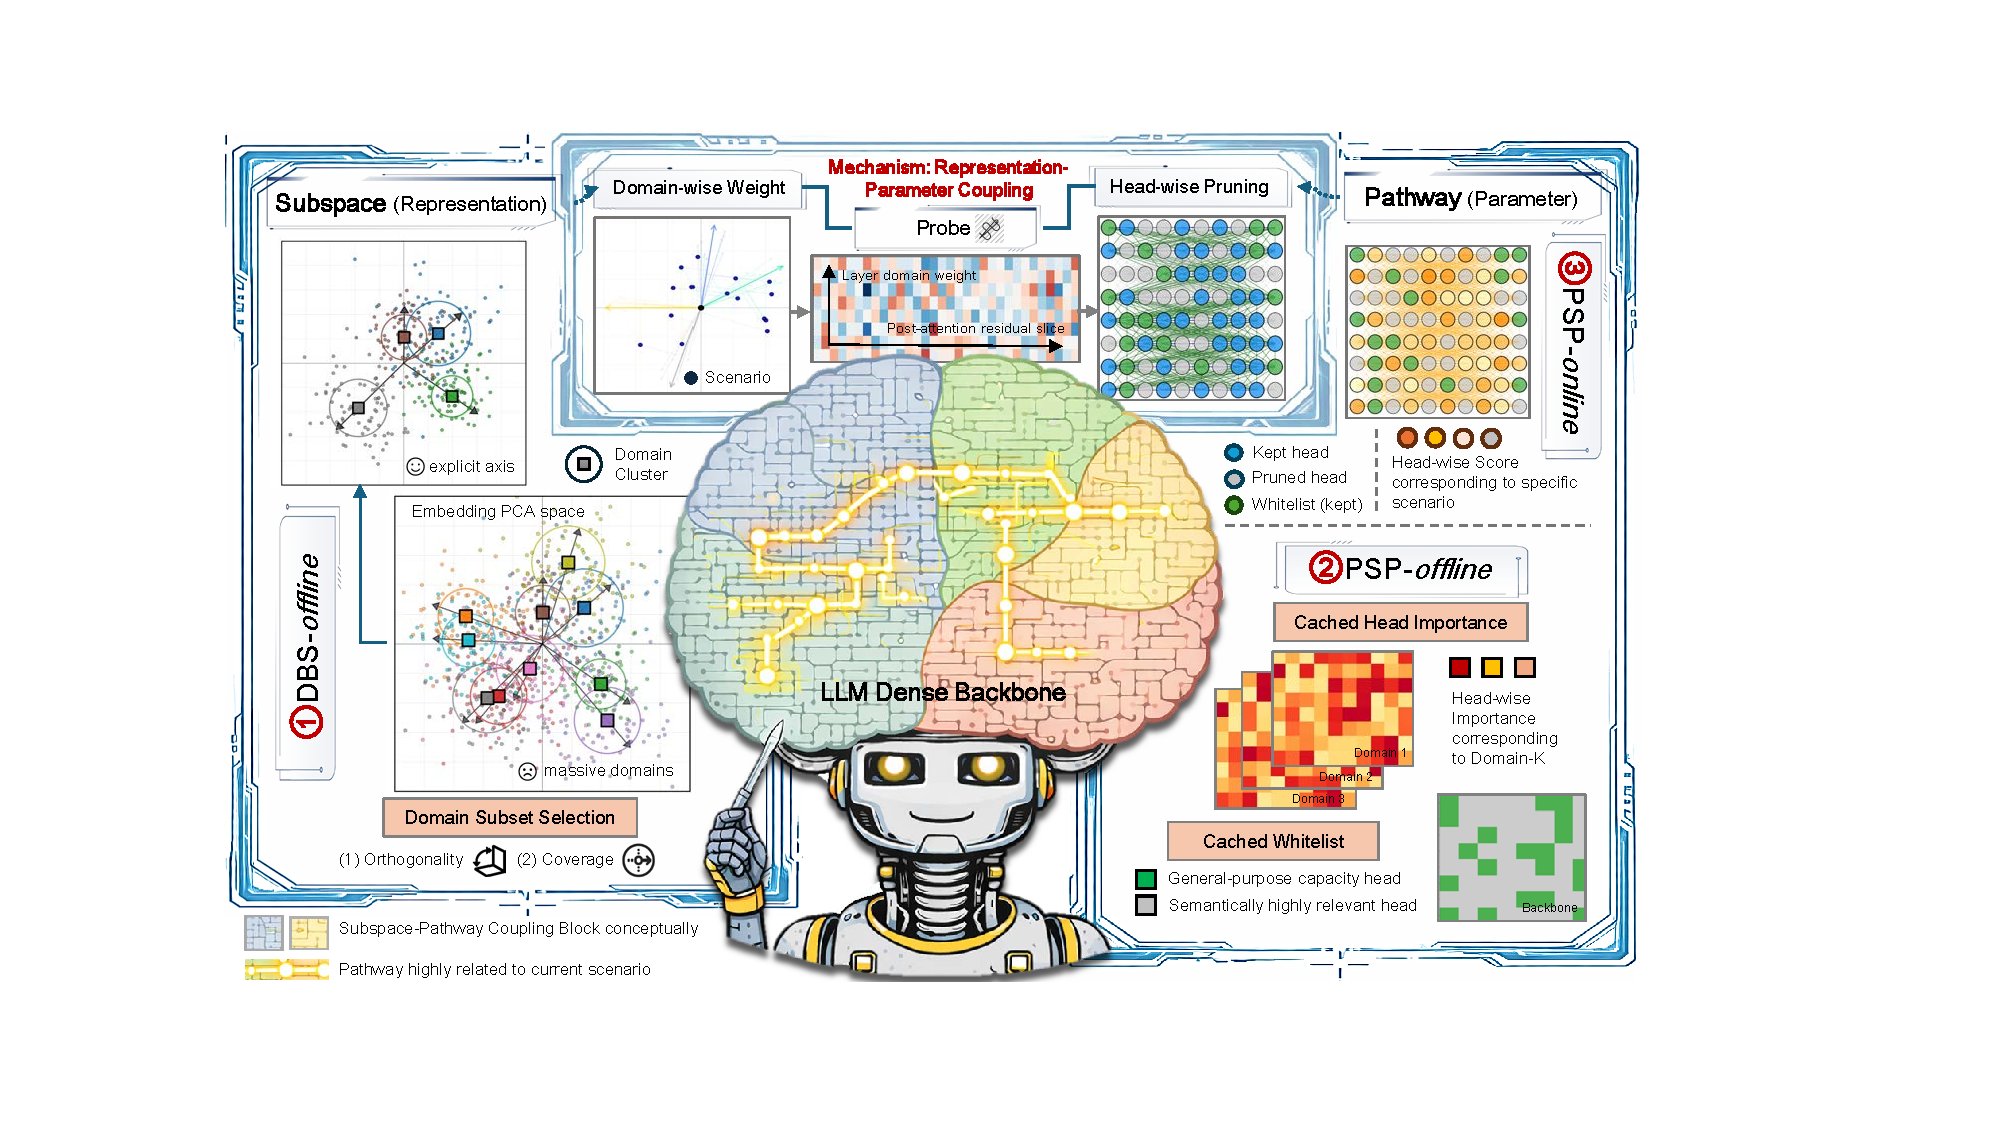
\includegraphics[width=0.95\textwidth]{sp_main.pdf}
\caption{\SubspacePath{} pipeline. Domain-Basis Synthesis builds a compact semantic coordinate system; Probe-based Scenario Pruning learns the representation--parameter coupling offline and compiles a scenario-specific head pathway online.}
\label{fig:subspace}
\end{figure}

\begin{methodbox}
\textbf{Input:} a frozen LLM, input-only domain pools available once offline, and an unseen deployment scenario. \quad
\textbf{Signal:} a compact semantic-domain basis read from residual-stream probes. \quad
\textbf{Coupling:} cached alignment between those semantic axes and attention-head writes. \quad
\textbf{Output:} a budgeted structured head mask plus a small always-retained general-purpose whitelist. \quad
\textbf{Online cost:} probe readout and top-$K$ compilation only; no scenario-specific training.
\end{methodbox}

\subsubsection{Representation side: a stable semantic coordinate}
Let the offline domain pools be $\{\mathcal P_k\}_{k\in\mathcal K}$. After embedding and PCA projection, each domain has a candidate unit direction $u_k$. Domain-Basis Synthesis selects a compact subset $\mathcal K_\star$ by balancing separation and coverage:
\begin{align}
\operatorname{Ortho}(\mathcal K')
&=1-\frac{2}{|\mathcal K'|(|\mathcal K'|-1)}\sum_{i<j}(u_i^\top u_j)^2,\label{eq:sp-ortho}\\
\operatorname{Cover}(\mathcal K')
&=\frac{\operatorname{tr}(\Pi(\mathcal K')\Sigma)}{\operatorname{tr}(\Sigma)},\label{eq:sp-cover}\\
J(\mathcal K')&=\lambda_{\rm ortho}\operatorname{Ortho}(\mathcal K')+\lambda_{\rm cov}\operatorname{Cover}(\mathcal K').\label{eq:sp-dbs}
\end{align}
Here $\Sigma$ is the pooled covariance in PCA space, $\Pi(\mathcal K')$ projects onto the axes, and $\lambda_{\rm ortho},\lambda_{\rm cov}$ trade off separation and coverage. Greedy screening stops at an elbow to obtain the basis $\mathbb U_\star=\{u_k:k\in\mathcal K_\star\}$.

The representation-side evidence is shown in Figure~\ref{fig:sp-repr-evidence}.
\begin{figure}[tbp]
\centering
\begin{subfigure}[b]{0.44\textwidth}
  \centering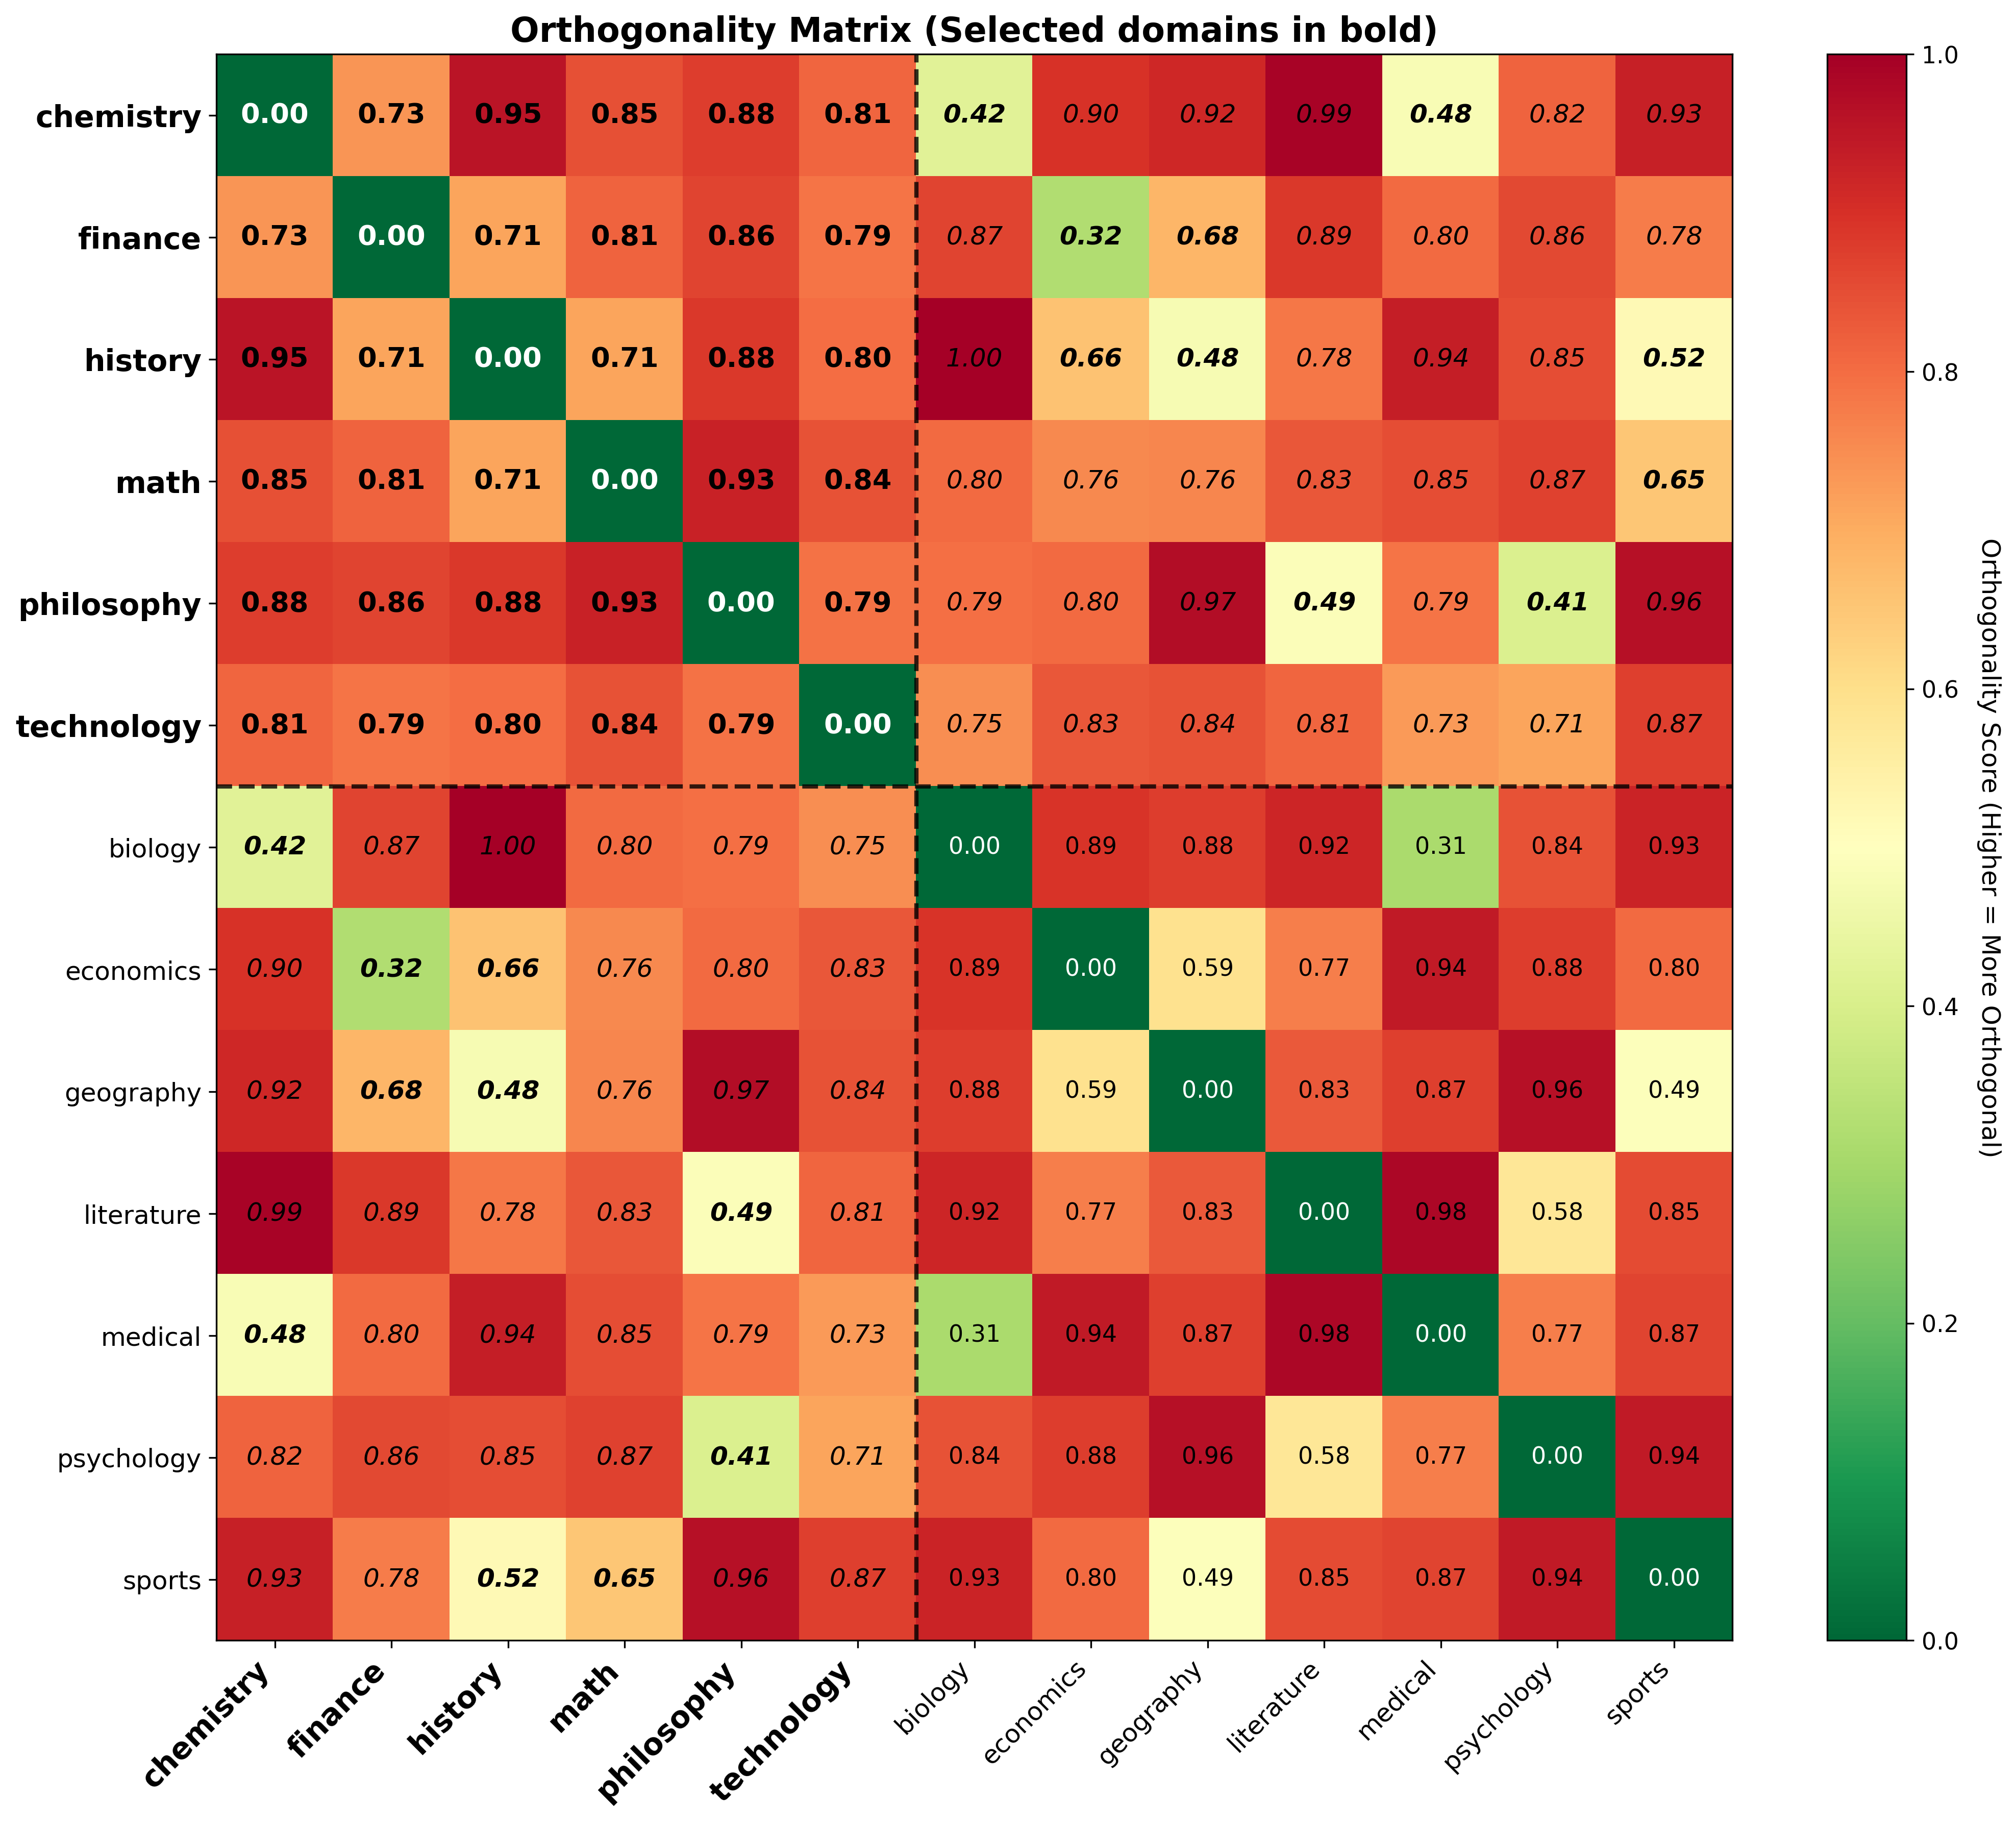
\includegraphics[width=\linewidth]{sp_domain_ortho.png}
\end{subfigure}\hfill
\begin{subfigure}[b]{0.44\textwidth}
  \centering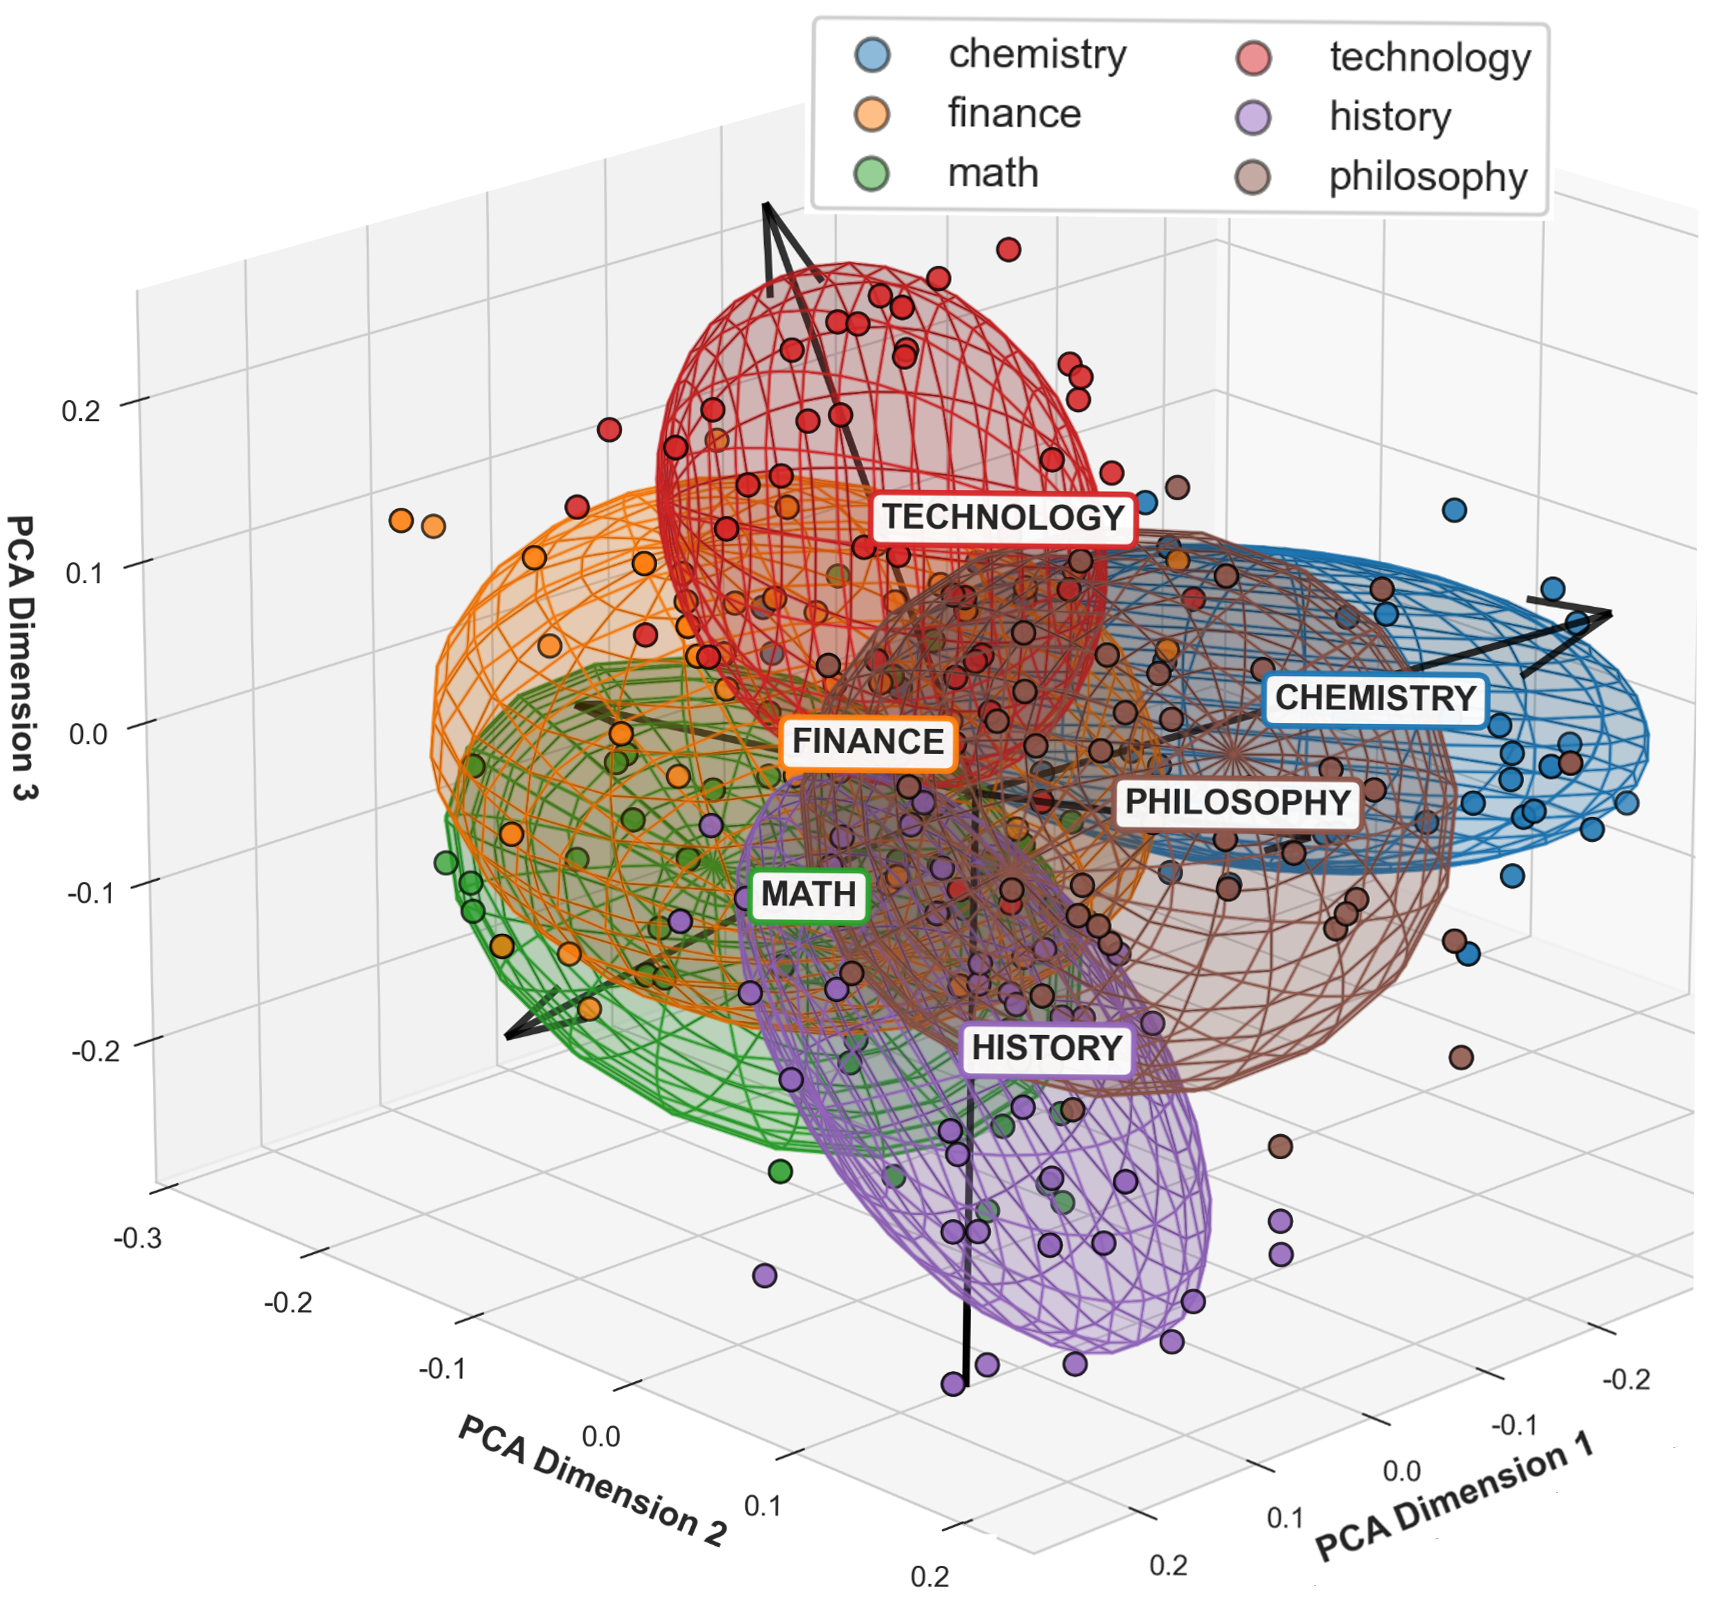
\includegraphics[width=\linewidth]{sp_domain_projection.png}
\end{subfigure}
\caption{Separation of domain representations in embedding space. \textbf{Left:} orthogonality heatmap across domains. \textbf{Right:} projection of the selected domain representations showing spatial separation. This empirical structure motivates using a compact semantic basis as the scenario coordinate.}
\label{fig:sp-repr-evidence}
\end{figure}

\subsubsection{Parameter side: representation--pathway coupling}
At layer $\ell$, lightweight probes read domain relevance from the post-attention residual slice $r^{(\ell)}(x)$:
\begin{equation}
p_{\ell,k}(x)=\sigma\!\left(g_{\ell,k}^{\top}r^{(\ell)}(\widetilde x)\right),
\label{eq:sp-probe}
\end{equation}
where $g_{\ell,k}$ is the probe for axis $k$ and $\widetilde x$ denotes the input representation used by the probe. Separately, let $w_{\ell,h}(x)$ be the residual-stream write of head $(\ell,h)$, projected into the same PCA coordinate. The cached coupling between domain axis $k$ and executable head $(\ell,h)$ is
\begin{equation}
I_{\ell,h,k}=\mathbb E_{x\sim\mathcal P_k}\!\left[
\frac{(u_k^\top\widetilde w_{\ell,h}(x))^2}{\|\widetilde w_{\ell,h}(x)\|_2^2+\epsilon}
\right].
\label{eq:sp-importance}
\end{equation}
The two sides now have a common interface: probes estimate which semantic axes are active; $I_{\ell,h,k}$ records which heads are coupled to those axes. A small whitelist $\mathcal W$ of low-variance, sufficiently important heads is retained across all scenarios to preserve domain-invariant capability.

Figure~\ref{fig:subspace-coupling} shows the representation-to-parameter bridge used by the compiler.
\begin{figure}[tbp]
\centering
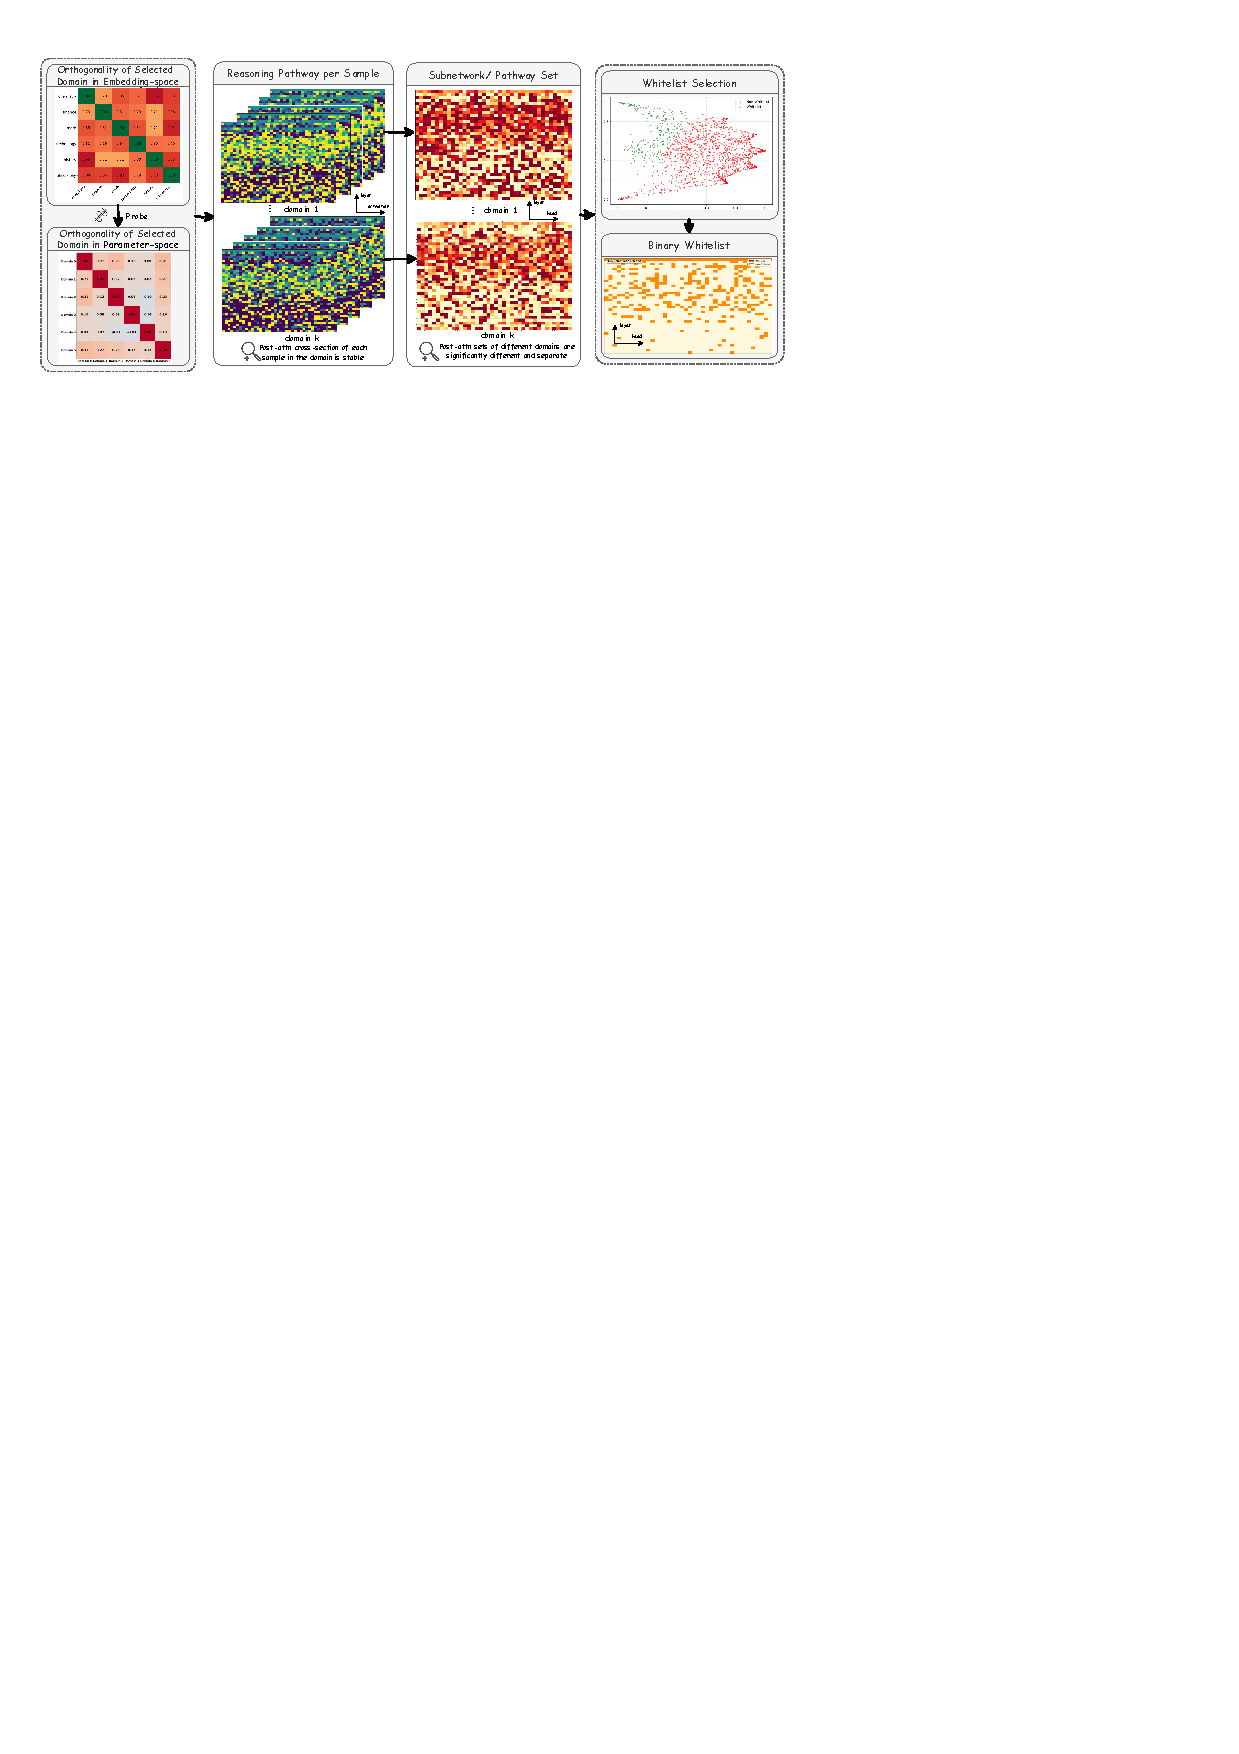
\includegraphics[width=0.95\textwidth]{sp_coupling_source.pdf}
\caption{Subspace--pathway coupling. Embedding-level domain axes are read from residual-stream slices by lightweight probes and linked to head-level pathway importance. The figure shows the representation-to-parameter bridge used by the online compiler.}
\label{fig:subspace-coupling}
\end{figure}

\subsubsection{Online compilation: scenario state to executable mask}
At scenario start, probe outputs are aggregated into a domain-mixture vector $q(s)$ over $\mathcal K_\star$. Its normalized entropy
\begin{equation}
c(s)=\frac{H(q(s))}{\log|\mathcal K_\star|}
\label{eq:sp-breadth}
\end{equation}
measures the breadth of the scenario. Before head scoring, the raw mixture $s_k=q_k(s)$ is nonlinearly sharpened so that highly relevant domains retain proportionally more capacity. Over the valid domain range $[s_{\min},s_{\max}]$,
\begin{equation}
\bar s_k=\frac{s_k-s_{\min}}{s_{\max}-s_{\min}},\qquad
s_k^{\rm eff}=s_{\min}+\bar s_k^{\,\gamma}(s_{\max}-s_{\min}),
\label{eq:sp-effective}
\end{equation}
with $\gamma=1.5$ in the reported experiments. The mixture then weights the cached head coupling,
\begin{equation}
\operatorname{score}_{\ell,h}(s)=\sum_{k\in\mathcal K_\star}s_k^{\rm eff}I_{\ell,h,k}.
\label{eq:sp-score}
\end{equation}
The retained head budget adapts with breadth,
\begin{equation}
K(s)=|\mathcal W|+\min\!\left\{K_B-|\mathcal W|,
\left\lceil(\rho_{\min}+\eta c(s))(|\mathcal H|-|\mathcal W|)\right\rceil\right\},
\label{eq:sp-budget}
\end{equation}
where $\mathcal H$ is the complete head set, $K_B$ is the maximum budget, $\rho_{\min}$ is the minimum retained fraction outside the whitelist, and $\eta$ controls how much additional capacity is allocated to broader scenarios. The mask is $\mathcal W$ plus the highest-scoring remaining heads. Nothing is optimized online: the compiled mask is reused over the coherent multi-turn scenario.

\subsubsection{Evaluation: cross-scenario generalization and physical efficiency}
The evaluation uses four LLM backbones and separates selected-domain, out-of-domain (OOD), cross-domain, and cross-dataset tests. Table~\ref{tab:sp-main} gives the detailed LLaMA-2-13B comparison, while Figure~\ref{fig:sp-radar} summarizes the model-average quality--efficiency profile and Figure~\ref{fig:sp-tradeoffs} shows how the useful operating point changes with pruning strength. This is central to the deployment claim: the method is not judged only on the distribution that produced the offline coupling, but on whether the compiler transfers when the scenario changes.

\begin{table}[t]
\centering\singlespacing
\caption{\SubspacePath{} on LLaMA-2-13B-chat across XDomainBench and cross-dataset tests. Recall is mean $\pm$ SEM. Retention combines quality with measured speedup, following the metric reported in the paper. The percentage row shows baseline pruning ratio $\sim$ the average ratio used by \SubspacePath{}.}
\label{tab:sp-main}
\setlength{\tabcolsep}{2.2pt}
\renewcommand{\arraystretch}{1.02}
\begin{adjustbox}{max width=\textwidth}
\begin{tabular}{llccc c ccc c}
\toprule
\textbf{Category} & \textbf{Method} &
\multicolumn{3}{c}{\textbf{XDomainBench Recall}} & \textbf{Retention} &
\multicolumn{3}{c}{\textbf{Cross-dataset Recall}} & \textbf{Retention}\\
\cmidrule(lr){3-5}\cmidrule(lr){6-6}\cmidrule(lr){7-9}\cmidrule(l){10-10}
&& \textbf{Selected} & \textbf{OOD} & \textbf{Cross} & \textbf{S/O/C} &
\textbf{CSQA} & \textbf{NQ} & \textbf{ARC} & \textbf{C/N/A}\\
\midrule
\rowcolor{SoftGray}\multicolumn{10}{c}{\textbf{Dense model}}\\
\multicolumn{2}{l}{LLaMA-2-13B} &
29.6{\scriptsize$\pm$1.45} & 26.1{\scriptsize$\pm$1.10} & 18.4{\scriptsize$\pm$0.74} &
1.00/1.00/1.00 &
22.27{\scriptsize$\pm$1.20} & 30.25{\scriptsize$\pm$1.07} & 23.87{\scriptsize$\pm$0.89} &
1.00/1.00/1.00\\
\midrule
\rowcolor{SoftGray}\multicolumn{10}{c}{\textbf{Moderate pruning}}\\
\rowcolor{SoftGray}&&
80\%$\sim$79.6\% & 89\%$\sim$88.4\% & 86\%$\sim$85.5\% && 
90\%$\sim$89.9\% & 82\%$\sim$81.5\% & 81\%$\sim$80.2\% &\\
\multirow{1}{*}{Unstruct.} & DaSS &
33.82{\scriptsize$\pm$1.56} & 28.62{\scriptsize$\pm$1.16} & 19.89{\scriptsize$\pm$0.79} &
0.42/0.49/0.50 &
20.10{\scriptsize$\pm$1.14} & 18.80{\scriptsize$\pm$0.96} & 19.22{\scriptsize$\pm$0.82} &
0.24/0.15/0.35\\
\multirow{2}{*}{Struct.} & Wanda &
26.87{\scriptsize$\pm$1.46} & 27.26{\scriptsize$\pm$1.14} & 15.43{\scriptsize$\pm$0.74} &
0.35/0.46/0.45 &
17.63{\scriptsize$\pm$1.09} & 17.27{\scriptsize$\pm$0.98} & 14.38{\scriptsize$\pm$0.75} &
0.18/0.11/0.24\\
& LLM-Pr. &
29.34{\scriptsize$\pm$1.49} & 27.81{\scriptsize$\pm$1.14} & 18.92{\scriptsize$\pm$0.75} &
0.95/1.02/0.99 &
21.08{\scriptsize$\pm$1.17} & 27.63{\scriptsize$\pm$1.14} & 23.09{\scriptsize$\pm$0.89} &
0.91/0.88/0.94\\
\multirow{2}{*}{Activ.} & RIA &
27.06{\scriptsize$\pm$1.47} & 27.03{\scriptsize$\pm$1.14} & 15.12{\scriptsize$\pm$0.73} &
0.36/0.47/0.46 &
17.98{\scriptsize$\pm$1.10} & 17.24{\scriptsize$\pm$0.98} & 14.33{\scriptsize$\pm$0.75} &
0.19/0.12/0.25\\
& Probe Pr. &
29.02{\scriptsize$\pm$1.58} & 27.81{\scriptsize$\pm$1.28} & 19.08{\scriptsize$\pm$1.12} &
1.22/1.33/1.24 &
21.75{\scriptsize$\pm$1.30} & 27.64{\scriptsize$\pm$1.41} & 23.32{\scriptsize$\pm$1.34} &
1.17/1.09/1.17\\
\rowcolor{SoftBlue}\multicolumn{2}{l}{\textbf{\SubspacePath{}}} &
\textbf{43.00{\scriptsize$\pm$2.40}} & \textbf{32.50{\scriptsize$\pm$1.90}} & \textbf{20.20{\scriptsize$\pm$3.00}} &
\textbf{1.48/1.56/1.78} &
19.43{\scriptsize$\pm$1.14} & \textbf{33.66{\scriptsize$\pm$1.35}} & 22.91{\scriptsize$\pm$1.08} &
0.94/\textbf{1.20}/\textbf{2.12}\\
\midrule
\rowcolor{SoftGray}\multicolumn{10}{c}{\textbf{Aggressive pruning}}\\
\rowcolor{SoftGray}&&
71\%$\sim$71.0\% & 83\%$\sim$82.8\% & 72\%$\sim$71.3\% &&
82\%$\sim$81.2\% & 70\%$\sim$69.5\% & 69\%$\sim$68.3\% &\\
\multirow{1}{*}{Unstruct.} & DaSS &
35.27{\scriptsize$\pm$1.57} & 27.84{\scriptsize$\pm$1.15} & 15.40{\scriptsize$\pm$0.71} &
0.87/0.84/0.80 &
18.13{\scriptsize$\pm$1.10} & 12.42{\scriptsize$\pm$0.75} & 16.29{\scriptsize$\pm$0.79} &
0.49/0.22/0.72\\
\multirow{2}{*}{Struct.} & Wanda &
18.12{\scriptsize$\pm$1.26} & 26.57{\scriptsize$\pm$1.15} & 8.77{\scriptsize$\pm$0.54} &
0.16/0.47/0.24 &
13.70{\scriptsize$\pm$0.99} & 8.09{\scriptsize$\pm$0.71} & 9.50{\scriptsize$\pm$0.64} &
0.17/0.06/0.31\\
& LLM-Pr. &
27.30{\scriptsize$\pm$1.46} & 28.15{\scriptsize$\pm$1.15} & 17.36{\scriptsize$\pm$0.71} &
0.60/1.05/0.61 &
21.20{\scriptsize$\pm$1.18} & 19.12{\scriptsize$\pm$0.95} & 21.01{\scriptsize$\pm$0.82} &
0.92/0.49/0.70\\
\multirow{2}{*}{Activ.} & RIA &
18.94{\scriptsize$\pm$1.28} & 26.69{\scriptsize$\pm$1.15} & 8.52{\scriptsize$\pm$0.54} &
0.33/0.91/0.45 &
12.48{\scriptsize$\pm$0.93} & 8.06{\scriptsize$\pm$0.71} & 9.75{\scriptsize$\pm$0.64} &
0.31/0.10/0.32\\
& Probe Pr. &
15.19{\scriptsize$\pm$1.25} & 27.84{\scriptsize$\pm$1.28} & 11.54{\scriptsize$\pm$0.91} &
0.43/1.29/0.52 &
21.65{\scriptsize$\pm$1.30} & 11.34{\scriptsize$\pm$1.00} & 6.96{\scriptsize$\pm$0.80} &
1.19/0.31/0.25\\
\rowcolor{SoftBlue}\multicolumn{2}{l}{\textbf{\SubspacePath{}}} &
\textbf{34.70{\scriptsize$\pm$2.30}} & \textbf{30.40{\scriptsize$\pm$1.90}} & \textbf{22.90{\scriptsize$\pm$3.20}} &
\textbf{1.24/1.36/1.92} &
18.40{\scriptsize$\pm$1.12} & \textbf{24.89{\scriptsize$\pm$1.22}} & \textbf{21.56{\scriptsize$\pm$1.04}} &
0.65/0.80/\textbf{1.59}\\
\bottomrule
\end{tabular}
\end{adjustbox}
\end{table}

\begin{figure}[tbp]
\centering
\begin{minipage}[c]{0.48\textwidth}
  \centering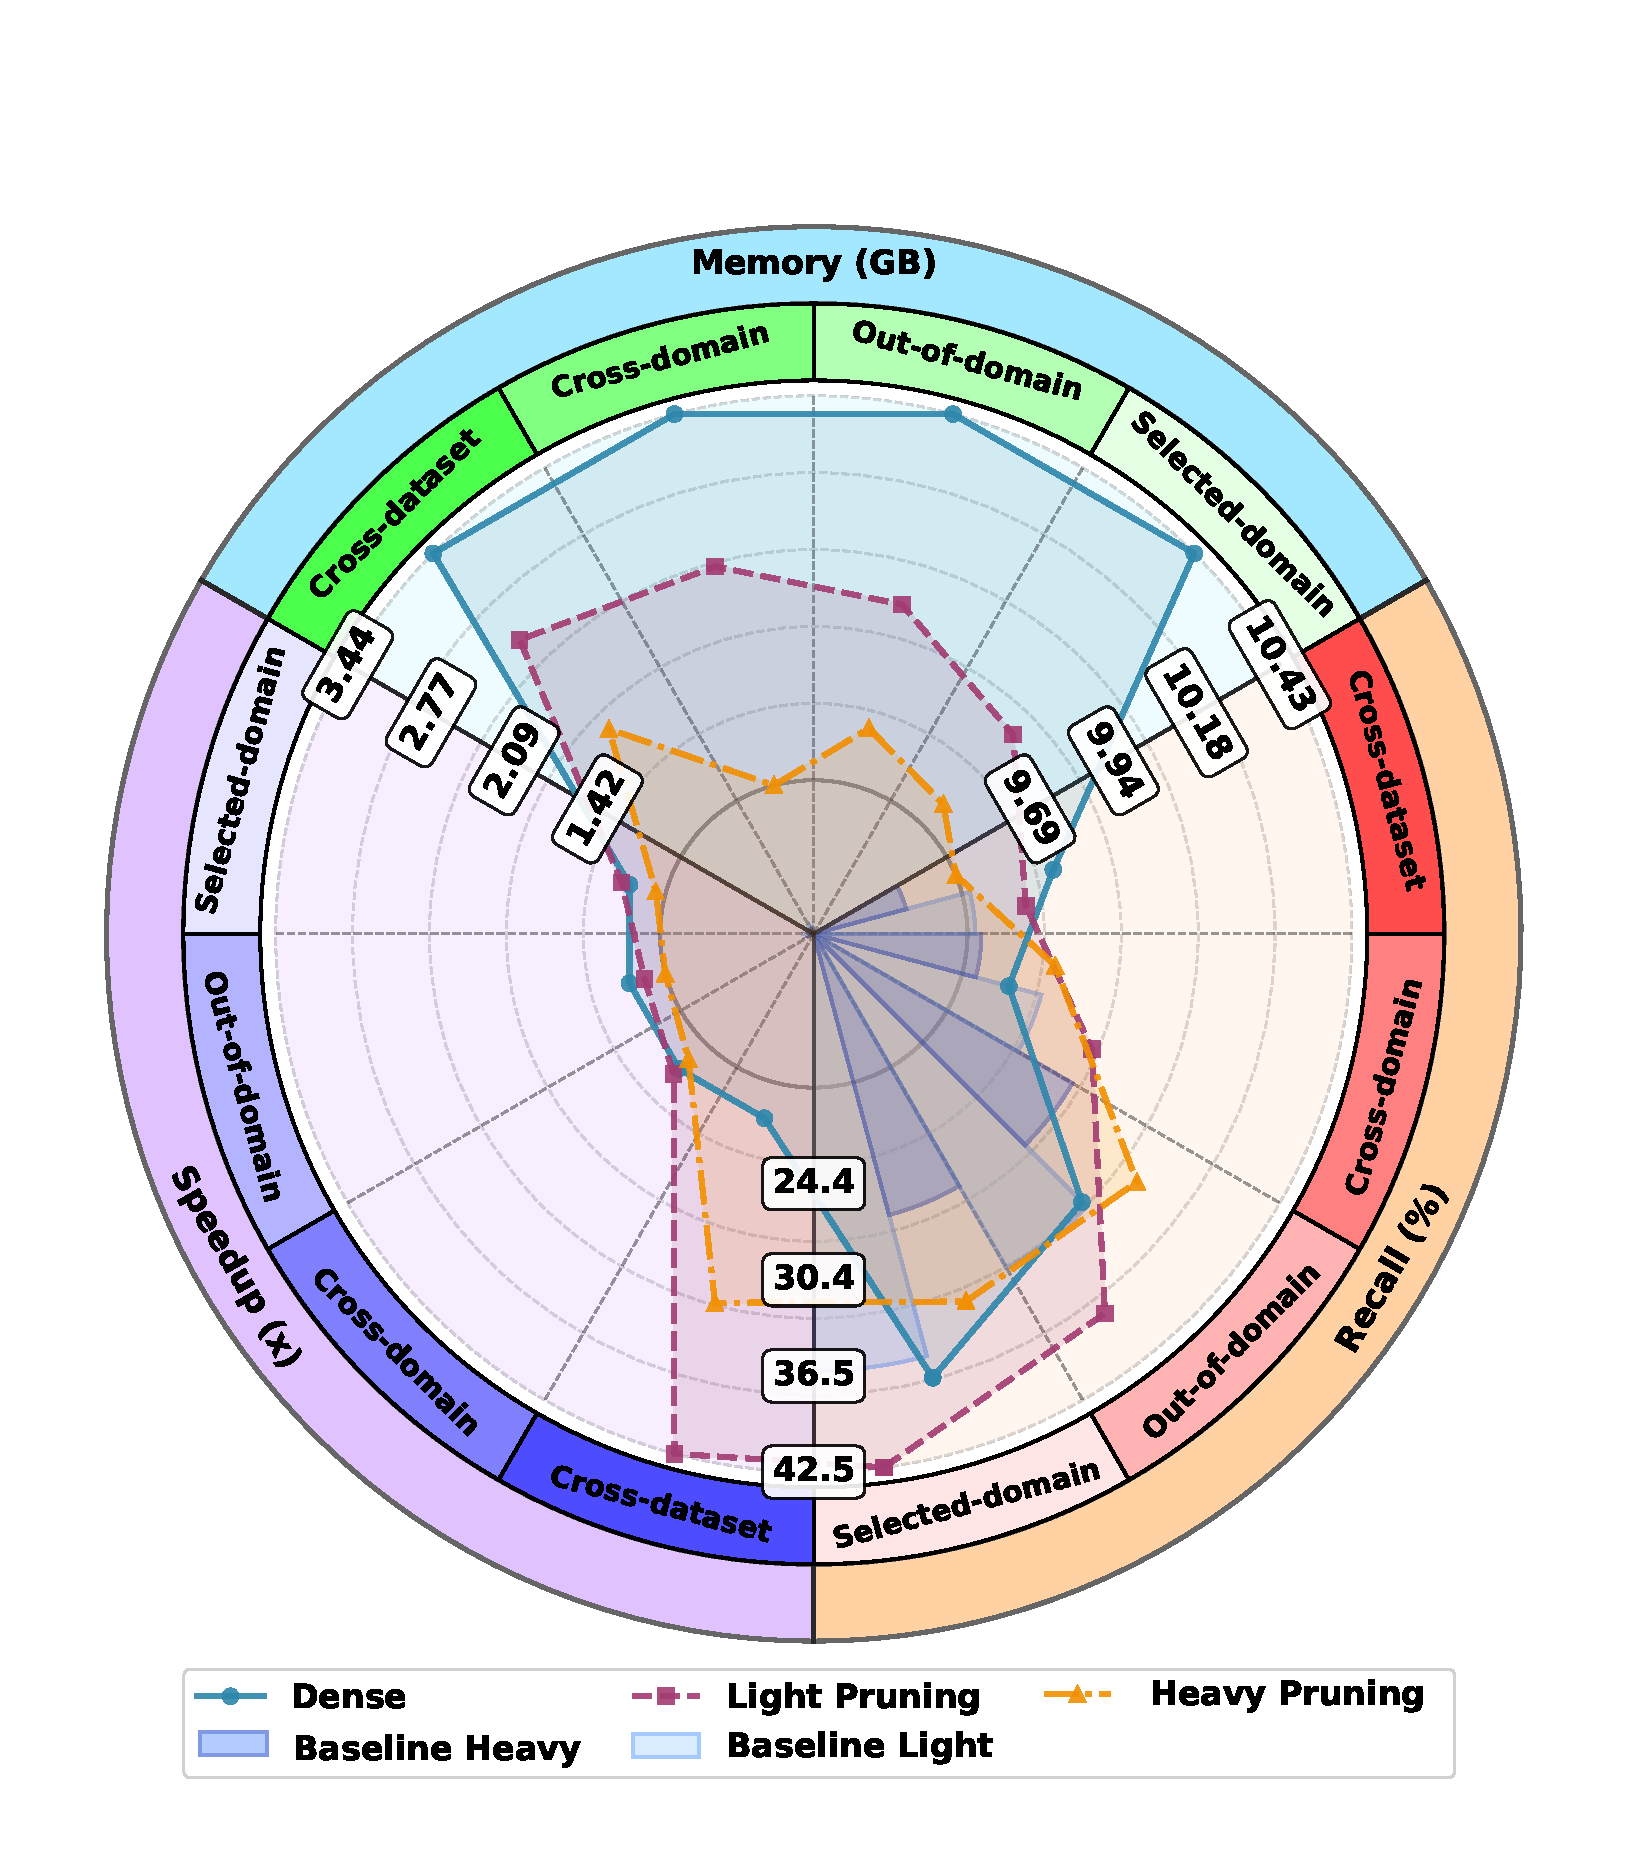
\includegraphics[width=0.94\linewidth]{sp_radar_source.pdf}
\end{minipage}\hfill
\begin{minipage}[c]{0.47\textwidth}
\small
\textbf{Model-average robustness.} The radar view jointly summarizes recall, memory, and measured speedup across selected-domain, OOD, cross-domain, and cross-dataset settings. Its main message is not a single best pruning ratio: the useful operating point changes with deployment condition, while scenario-conditioned masks preserve substantially more capability under shift.
\end{minipage}
\caption{Model-average quality--efficiency profile of \SubspacePath{} across models and evaluation settings.}
\label{fig:sp-radar}
\end{figure}

\begin{figure}[tbp]
\centering
\begin{subfigure}[t]{0.48\textwidth}
\centering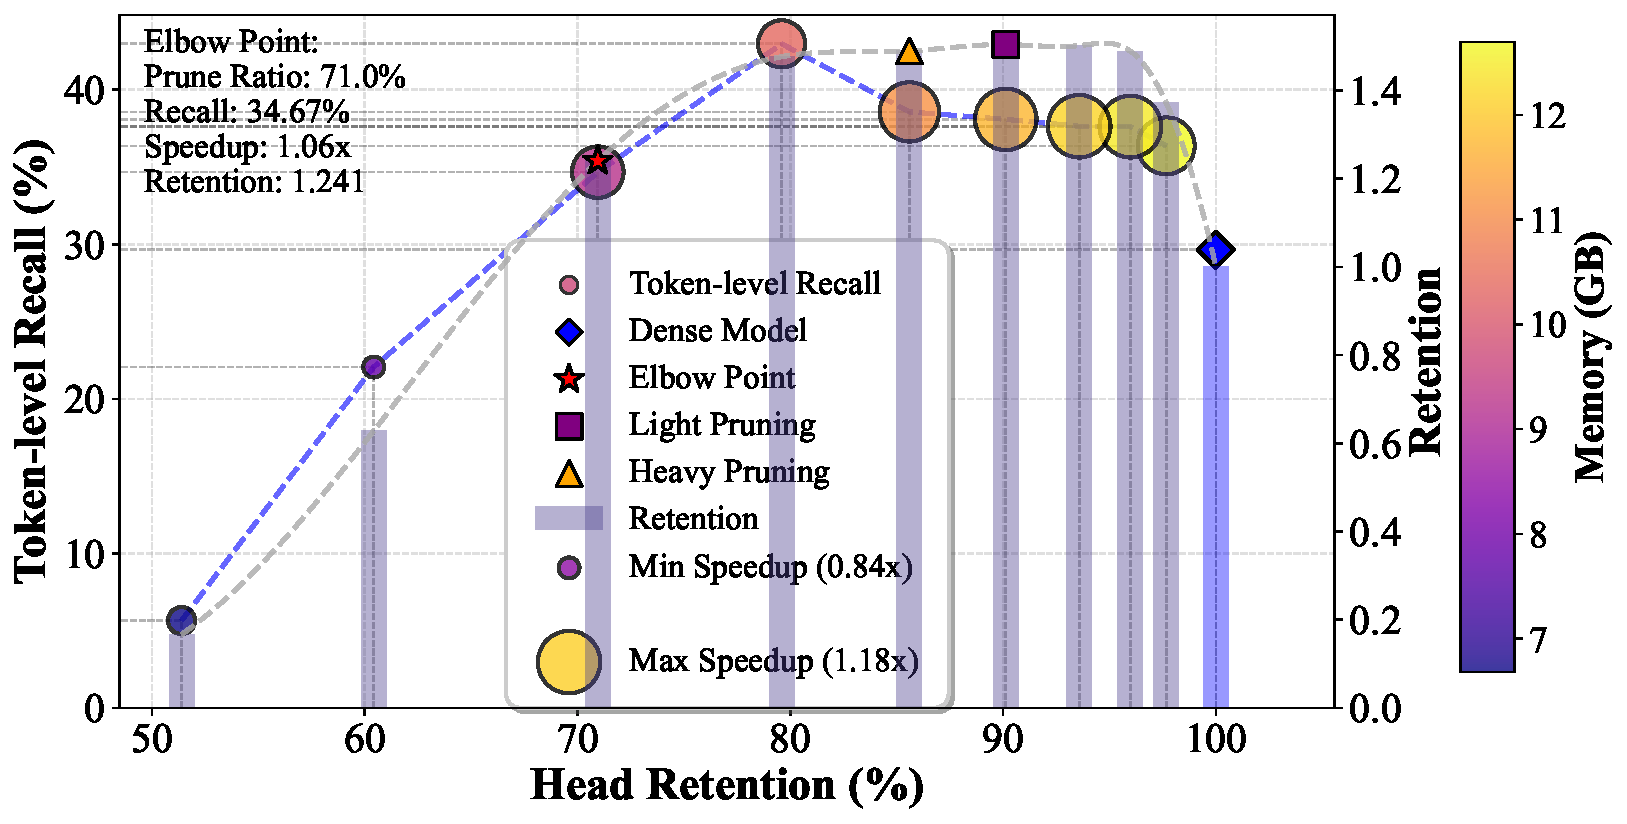
\includegraphics[width=\linewidth]{pruning_tradeoff_LLaMA_13B_xdomainbench_avg.pdf}
\caption{XDomainBench average}
\end{subfigure}\hfill
\begin{subfigure}[t]{0.48\textwidth}
\centering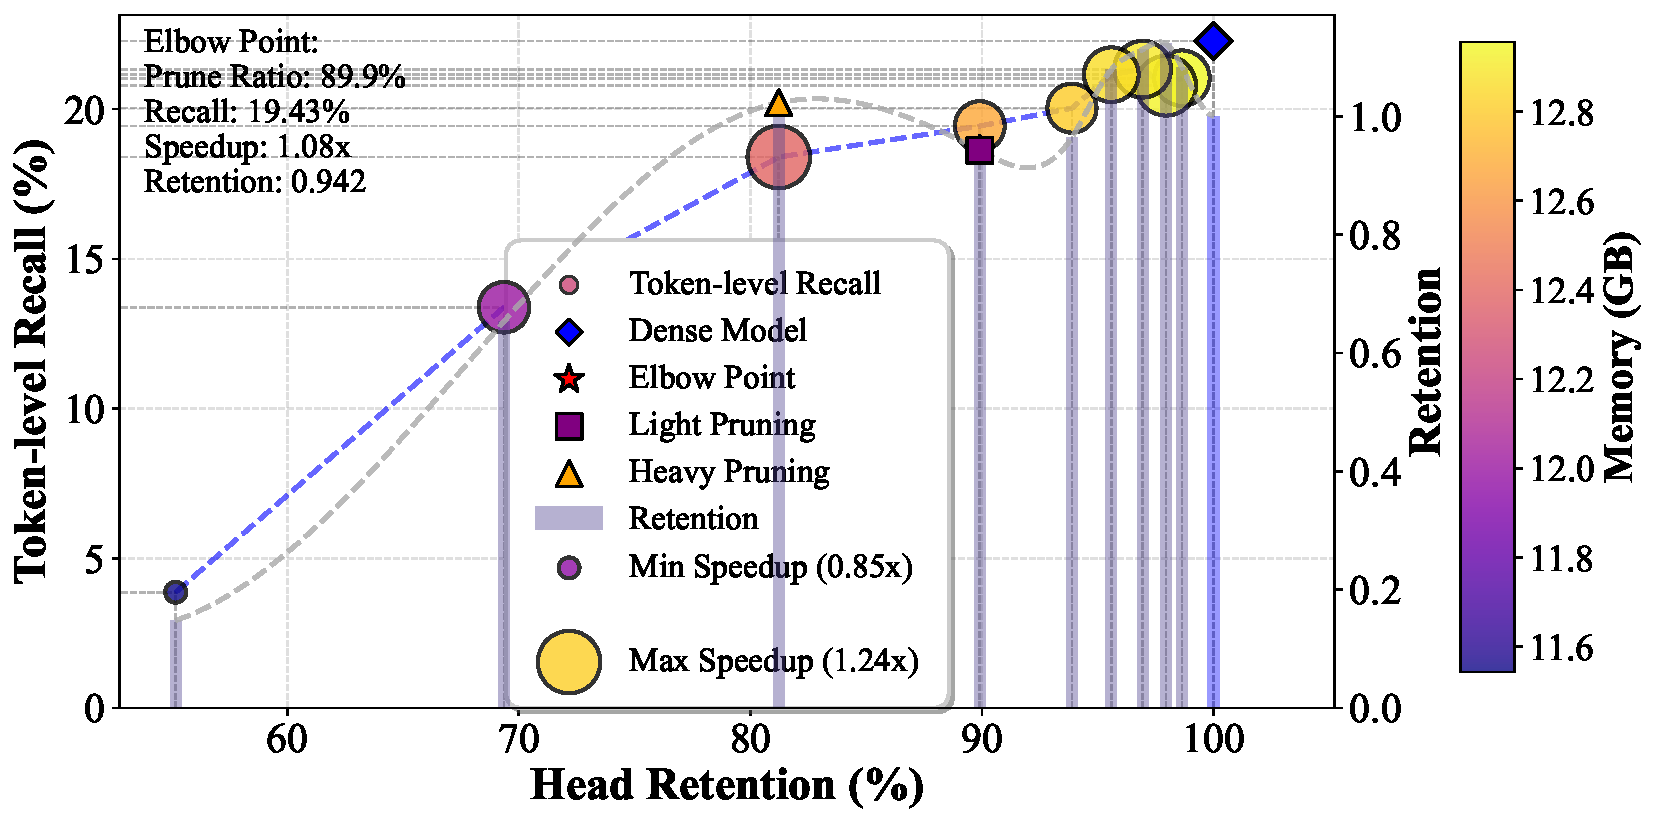
\includegraphics[width=\linewidth]{pruning_tradeoff_LLaMA_13B_csqa.pdf}
\caption{CommonsenseQA}
\end{subfigure}
\vspace{2mm}
\begin{subfigure}[t]{0.48\textwidth}
\centering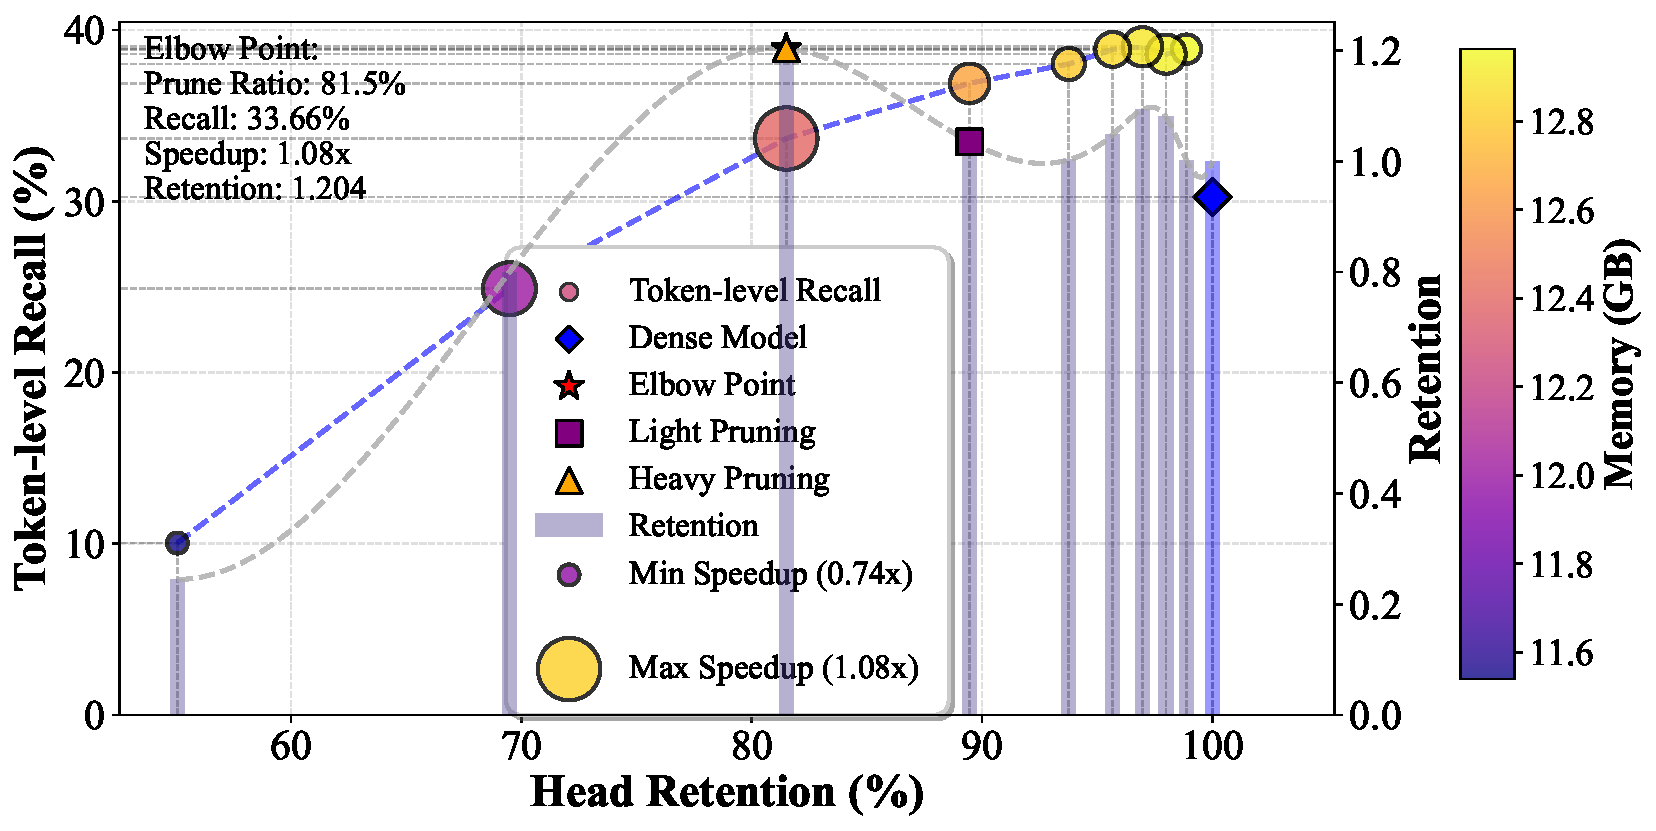
\includegraphics[width=\linewidth]{pruning_tradeoff_LLaMA_13B_nq.pdf}
\caption{Natural Questions}
\end{subfigure}\hfill
\begin{subfigure}[t]{0.48\textwidth}
\centering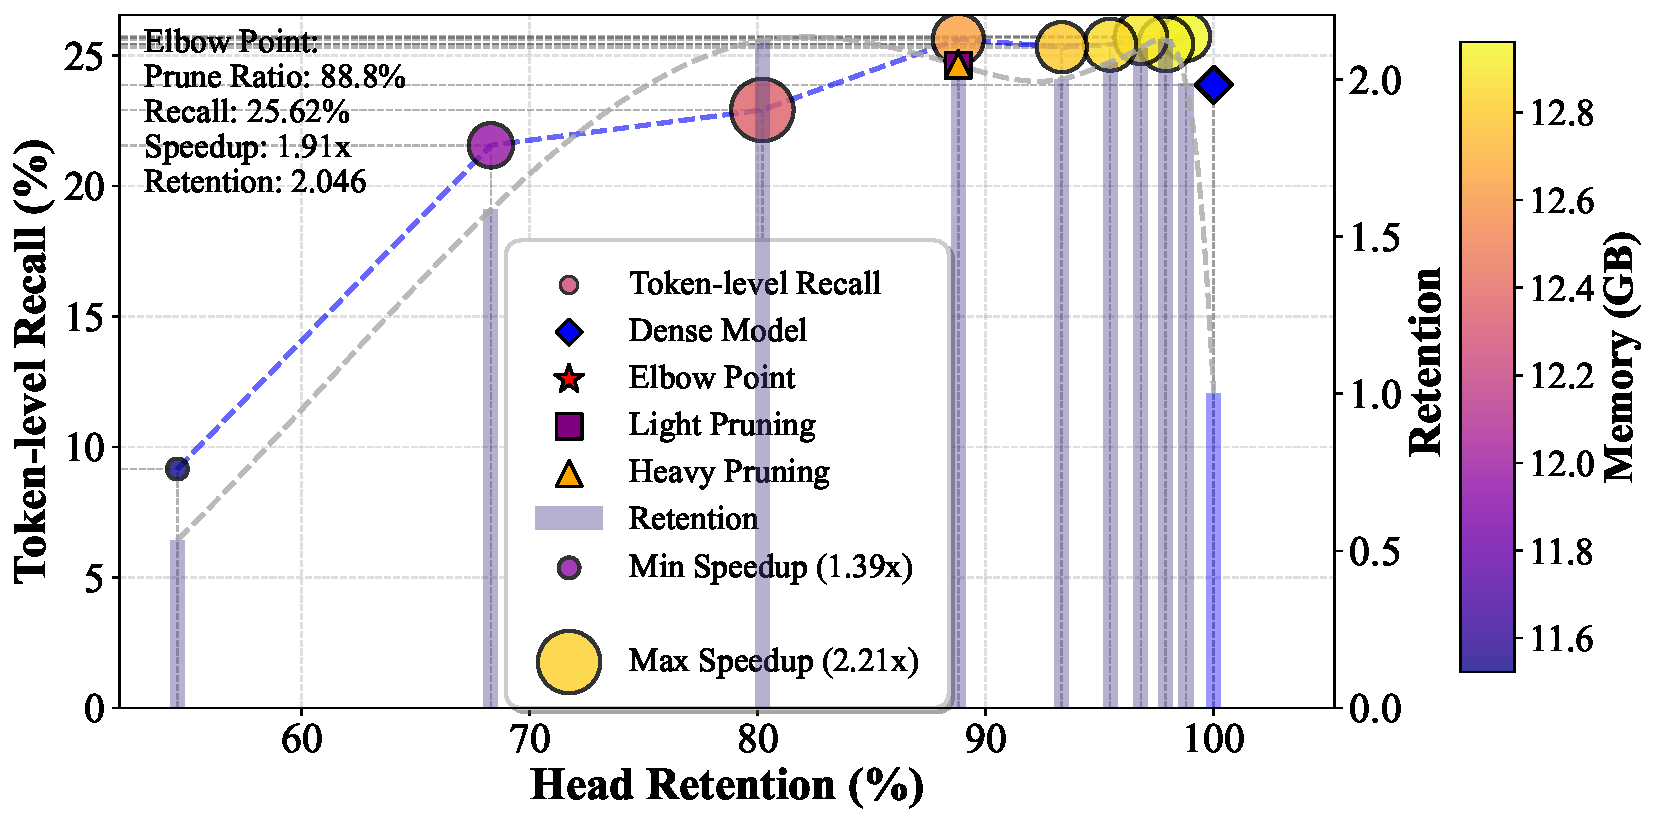
\includegraphics[width=\linewidth]{pruning_tradeoff_LLaMA_13B_arc.pdf}
\caption{ARC}
\end{subfigure}
\caption{Pruning ratio versus Recall for LLaMA-2-13B under different pruning strengths, compared with the dense model. The four panels show that the useful pruning range depends strongly on the deployment distribution and task, motivating scenario-level rather than globally fixed operating points.}
\label{fig:sp-tradeoffs}
\end{figure}

Table~\ref{tab:sp-crossmodel} extends the quality comparison across four backbones.
\begin{table}[tbp]
\centering\singlespacing\scriptsize
\caption{Cross-backbone moderate-pruning results. For each backbone, the strongest non-\SubspacePath{} pruning result is shown separately from the dense checkpoint. ``SP retention'' gives the approximate head-retention operating point for Selected/OOD/Cross/NQ, making the comparison interpretable as a quality--sparsity result rather than a raw accuracy table.}
\label{tab:sp-crossmodel}
\setlength{\tabcolsep}{3.0pt}\renewcommand{\arraystretch}{1.05}
\begin{adjustbox}{max width=\textwidth}
\begin{tabular}{llrrrrl}
\toprule
\textbf{Backbone} & \textbf{Selector} & \textbf{Selected} & \textbf{OOD} & \textbf{Cross} & \textbf{NQ} & \textbf{SP head retention (S/O/C/NQ)}\\
\midrule
\multirow{3}{*}{LLaMA-3.1-8B} & Dense & 39.1 & 33.2 & 21.3 & 28.82 & --\\
& Best pruning baseline & 34.09 & 27.68 & 19.36 & 25.85 & --\\
\rowcolor{SoftBlue}& \textbf{\SubspacePath{}} & 33.0 & \textbf{35.0} & \textbf{28.4} & \textbf{32.02} & $\sim$88.6/89.6/87.8/85.4\%\\
\midrule
\multirow{3}{*}{LLaMA-2-13B} & Dense & 29.6 & 26.1 & 18.4 & 30.25 & --\\
& Best pruning baseline & 33.82 & 28.62 & 19.89 & 27.64 & --\\
\rowcolor{SoftBlue}& \textbf{\SubspacePath{}} & \textbf{43.0} & \textbf{32.5} & \textbf{20.2} & \textbf{33.66} & $\sim$79.6/88.4/85.5/81.5\%\\
\midrule
\multirow{3}{*}{Qwen2.5-7B} & Dense & 40.8 & 33.6 & 22.9 & 17.51 & --\\
& Best pruning baseline & 33.53 & 30.56 & 19.99 & 13.65 & --\\
\rowcolor{SoftBlue}& \textbf{\SubspacePath{}} & \textbf{46.4} & \textbf{41.0} & \textbf{27.2} & \textbf{19.51} & $\sim$81.3/84.9/84.0/82.4\%\\
\midrule
\multirow{3}{*}{Qwen2.5-14B} & Dense & 40.9 & 37.2 & 22.8 & 19.72 & --\\
& Best pruning baseline & 42.97 & 38.07 & 22.18 & 19.63 & --\\
\rowcolor{SoftBlue}& \textbf{\SubspacePath{}} & \textbf{47.8} & \textbf{44.1} & \textbf{31.3} & \textbf{27.21} & $\sim$82.2/84.4/82.4/80.3\%\\
\bottomrule
\end{tabular}
\end{adjustbox}
\end{table}

Table~\ref{tab:sp-runtime} reports pruning cost and measured speedup against the same family of baselines.
\begin{table}[tbp]
\centering\singlespacing\scriptsize
\caption{Pruning time and measured speedup across methods and backbones. Pruning time is mean $\pm$ SEM over pruning ratios; speedup is reported as light/aggressive pruning, averaged over six datasets. \SubspacePath{} separates reusable offline preparation from lightweight per-scenario compilation.}
\label{tab:sp-runtime}
\setlength{\tabcolsep}{2.4pt}\renewcommand{\arraystretch}{1.04}
\begin{adjustbox}{max width=\textwidth}
\begin{tabular}{lrrrrl}
\toprule
\textbf{Pruning time (s)$\downarrow$} & \textbf{LLaMA-3.1-8B} & \textbf{LLaMA-2-13B} & \textbf{Qwen2.5-7B} & \textbf{Qwen2.5-14B} & \textbf{Method type}\\
\midrule
SparseGPT & 287.842{\scriptsize$\pm$2.683} & 403.481{\scriptsize$\pm$5.952} & 282.518{\scriptsize$\pm$2.961} & 487.479{\scriptsize$\pm$1.891} & one-shot unstructured\\
DaSS & 0.181{\scriptsize$\pm$0.079} & 0.567{\scriptsize$\pm$0.108} & 0.142{\scriptsize$\pm$0.090} & 0.613{\scriptsize$\pm$0.111} & dependency-aware\\
Wanda & 0.137{\scriptsize$\pm$0.109} & 0.525{\scriptsize$\pm$0.164} & 0.098{\scriptsize$\pm$0.067} & 0.558{\scriptsize$\pm$0.207} & structured\\
LLM-Pruner & 0.340{\scriptsize$\pm$0.055} & 0.593{\scriptsize$\pm$0.158} & 0.266{\scriptsize$\pm$0.032} & 0.599{\scriptsize$\pm$0.099} & gradient structured\\
RIA & 0.083{\scriptsize$\pm$0.033} & 0.275{\scriptsize$\pm$0.107} & 0.078{\scriptsize$\pm$0.031} & 0.290{\scriptsize$\pm$0.078} & activation-guided\\
Probe Pr. & 0.504{\scriptsize$\pm$0.007} & 0.715{\scriptsize$\pm$0.009} & 0.427{\scriptsize$\pm$0.045} & 0.845{\scriptsize$\pm$0.008} & probe-based\\
\rowcolor{SoftBlue}\textbf{\SubspacePath{}} & \textbf{0.039{\scriptsize$\pm$0.011}} & \textbf{0.060{\scriptsize$\pm$0.013}} & \textbf{0.027{\scriptsize$\pm$0.009}} & \textbf{0.068{\scriptsize$\pm$0.009}} & reusable offline + per scenario\\
\midrule
\textbf{Measured speedup$\uparrow$} & \textbf{LLaMA-3.1-8B} & \textbf{LLaMA-2-13B} & \textbf{Qwen2.5-7B} & \textbf{Qwen2.5-14B} & \textbf{light/aggressive}\\
\midrule
SparseGPT & 1.01/1.00 & 0.99/1.00 & 1.01/1.00 & 1.01/0.99 & --\\
DaSS & 0.72/0.55 & 0.40/0.83 & 0.53/0.45 & 0.63/1.07 & --\\
Wanda & 0.48/0.19 & 0.39/0.42 & 0.22/0.13 & 0.28/0.32 & --\\
LLM-Pruner & 0.61/0.64 & 0.96/0.80 & 0.66/0.67 & 0.96/0.66 & --\\
RIA & 0.36/0.19 & 0.40/0.74 & 0.13/0.29 & 0.29/0.32 & --\\
Probe Pr. & 0.77/0.77 & 1.25/0.96 & 1.25/0.82 & 1.10/0.74 & --\\
\rowcolor{SoftBlue}\textbf{\SubspacePath{}} & \textbf{1.41/1.35} & \textbf{3.22/1.51} & \textbf{2.01/0.88} & \textbf{1.38/1.29} & --\\
\bottomrule
\end{tabular}
\end{adjustbox}
\end{table}


The main pattern is strongest under distribution shift: the scenario-conditioned compiler improves Selected/OOD/Cross performance where one global ranking is least appropriate, and under aggressive pruning it retains cross-domain robustness while several baselines collapse. Compilation itself is lightweight---0.027--0.068 s across the evaluated 7B--14B backbones---and is paid once per coherent scenario.

Table~\ref{tab:sp-eff} separates retained-head ratio, model memory, and realized speedup on the physically executed model.
\begin{table}[tbp]
\centering\singlespacing\scriptsize
\caption{Measured efficiency for LLaMA-2-13B after structured head removal. ``Ret.'' is head retention, ``Mem.'' is peak model memory (GB), and ``Spd.'' is measured speedup.}
\label{tab:sp-eff}
\setlength{\tabcolsep}{2.0pt}
\begin{tabular}{@{}c@{\hspace{0.25em}}c@{\hspace{0.25em}}c@{\hspace{0.25em}}c@{}}
\begin{tabular}{lccc}\toprule
\multicolumn{4}{c}{\textbf{XDomainBench avg.}}\\\midrule
Type & Ret. & Mem. & Spd.\\\midrule Dense&--&13.0&1.00\\ Light&80.7\%&12.1&1.26\\ Heavy&72.2\%&11.7&1.24\\\bottomrule\end{tabular}&
\begin{tabular}{lccc}\toprule
\multicolumn{4}{c}{\textbf{CSQA}}\\\midrule
Type & Ret. & Mem. & Spd.\\\midrule Dense&--&13.0&1.00\\ Light&89.9\%&12.7&1.08\\ Heavy&69.4\%&12.0&1.09\\\bottomrule\end{tabular}&
\begin{tabular}{lccc}\toprule
\multicolumn{4}{c}{\textbf{NQ}}\\\midrule
Type & Ret. & Mem. & Spd.\\\midrule Dense&--&13.0&1.00\\ Light&81.5\%&12.4&1.08\\ Heavy&69.5\%&12.0&0.97\\\bottomrule\end{tabular}&
\begin{tabular}{lccc}\toprule
\multicolumn{4}{c}{\textbf{ARC}}\\\midrule
Type & Ret. & Mem. & Spd.\\\midrule Dense&--&13.0&1.00\\ Light&80.2\%&12.4&2.21\\ Heavy&68.3\%&12.0&1.76\\\bottomrule\end{tabular}
\end{tabular}
\end{table}

\textbf{What makes the compiler work?} The ablation isolates each link in the representation-to-pathway chain. Randomizing the semantic axes destroys the coordinate; removing the whitelist removes broadly useful computation under shift; removing multi-domain mixing weakens complex-scenario transfer.

Table~\ref{tab:sp-ablation} isolates the representation, whitelist, and multi-domain components of the compiler.
\begin{table}[tbp]
\centering\singlespacing\footnotesize
\caption{Coupling ablation on LLaMA-2-13B at the paper's elbow points (Recall, \%).}
\label{tab:sp-ablation}
\setlength{\tabcolsep}{3.2pt}
\begin{tabular}{lrrrrrr}
\toprule
\textbf{Variant} & \textbf{Sel.} & \textbf{OOD} & \textbf{Cross} & \textbf{CSQA} & \textbf{NQ} & \textbf{ARC}\\
\midrule
Dense & 29.6 & 26.1 & 18.4 & 22.27 & 30.25 & 23.87\\
Full: DBS + PSP & \textbf{34.7} & \textbf{30.4} & \textbf{22.9} & 19.43 & \textbf{33.66} & \textbf{25.62}\\
w/o DBS selection (random axes) & 1.8 & 1.4 & 0.9 & 0.82 & 0.40 & 1.16\\
w/o whitelist & 22.4 & 0.4 & 20.2 & 0.10 & 0.12 & 0.23\\
w/o multi-domain mixing & 29.5 & 23.5 & 19.0 & 7.07 & 10.68 & 17.04\\
\bottomrule
\end{tabular}
\end{table}

These results close the technical loop. The gain does not come from simply using fewer heads: it depends on a stable semantic coordinate, readable scenario state, an empirically supported coupling to executable head pathways, and a small domain-invariant backbone. In other words, pruning becomes a scenario-level controller rather than a static ranking.

\begin{insightbox}
\textbf{What \SubspacePath{} adds to the thesis.} The first technical step makes an external deployment condition executable inside the model. It establishes the basic adaptive-computation pattern used throughout the report: \emph{read a compact state, couple it to internal computation, and compile only what the current scenario needs}.
\end{insightbox}

\subsection{Interaction-Aware Structured Compression with \CoCurve{} \texorpdfstring{\projecticon{https://gongzhiren.github.io/CoCurve-website/}}{}}
\label{sec:cocurve}

\textbf{From scenario specialization to model-wide redundancy.} \SubspacePath{} shows that model execution should depend on the deployment scenario. The next step is broader: given a scenario-independent goal of compressing the \emph{whole} model, how should structured units be selected when attention and FFN computation interact through a shared residual stream? The self-repair behavior observed in \CoAx{} provides a useful warning---the effect of one component can depend on what else remains active. \CoCurve{} turns that observation into a compression objective by replacing scalar node importance with an output-grounded interaction matrix whose diagonal captures individual saliency and whose off-diagonal captures additional co-pruning damage~\citep{gong2026cocurve}.

Figure~\ref{fig:cocurve} gives the end-to-end view of the estimator, selector, and physically sliced output model.
\begin{figure}[tbp]
\centering
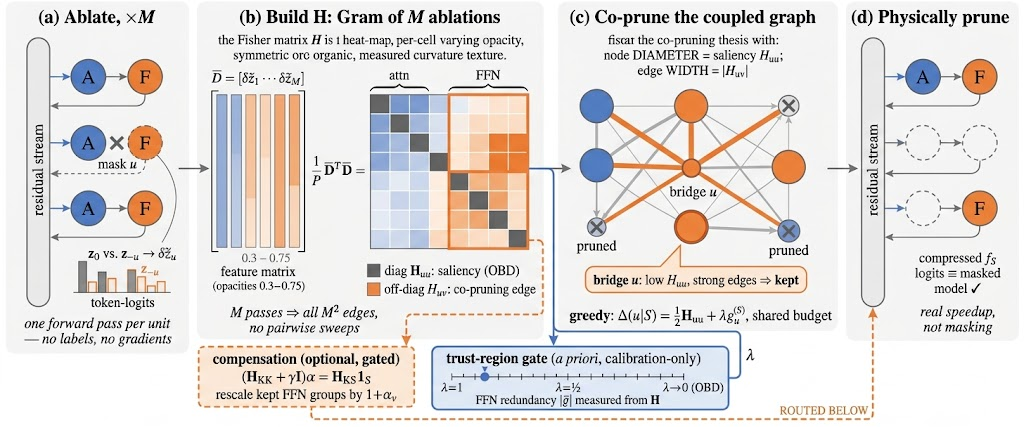
\includegraphics[width=0.98\textwidth]{cocurve_user.png}
\caption{\CoCurve{} overview. Single-unit output perturbations are assembled into a co-pruning curvature matrix; the interaction-aware selector operates under one shared structured budget and exports a physically smaller model~\citep{gong2026cocurve}.}
\label{fig:cocurve}
\end{figure}

\subsubsection{Structured pruning as a set-risk problem}
Let $\mathcal U=\{u_1,\ldots,u_M\}$ be removable structured units spanning attention heads and FFN groups. With removal indicator $s\in\{0,1\}^M$, define a label-free self-distillation risk between the frozen model $p_0$ and masked model $p_s$ on unlabeled calibration text:
\begin{equation}
\mathcal R(s)=\mathbb E_{x\in\mathcal C}\left[
\frac{1}{|\mathcal T(x)|}\sum_t
\operatorname{KL}\!\left(p_0(\cdot|x,t)\Vert p_s(\cdot|x,t)\right)
\right].
\label{eq:cc-risk}
\end{equation}
At zero pruning, $\mathcal R(0)=0$ and $\nabla\mathcal R(0)=0$. Let $H=\nabla^2\mathcal R(0)$ denote the Hessian of the pruning risk at the dense model. The leading local term is therefore second order:
\begin{equation}
\mathcal R(s)\approx \frac12 s^\top H s
=\frac12\sum_u H_{uu}s_u+\sum_{u<v}H_{uv}s_us_v.
\label{eq:cc-quadratic}
\end{equation}
This decomposition makes the conceptual change explicit. $H_{uu}$ is the familiar node saliency; $H_{uv}$ is the extra output risk associated with removing $u$ and $v$ together. Dropping every off-diagonal recovers a structured Optimal-Brain-Damage-style objective. \CoCurve{} therefore contains node-wise pruning as a diagonal special case rather than competing with it as an unrelated score.

\subsubsection{Estimating all pairwise edges from only $M$ single-unit ablations}
Naively measuring every pair would require $O(M^2)$ ablation sweeps. The key estimator avoids that cost. At calibration token $p$, let $\delta z_{u,p}$ be the logit perturbation caused by ablating unit $u$, let $q_p$ be the clean next-token distribution, and define its categorical Fisher matrix
\begin{equation}
F_p=\operatorname{Diag}(q_p)-q_pq_p^\top .
\label{eq:cc-fisher}
\end{equation}
A Fisher-whitened perturbation feature $d_{u,p}=F_p^{1/2}\delta z_{u,p}$ is stacked over the $P$ calibration positions to form column $\bar D_u=[d_{u,1};\ldots;d_{u,P}]$. Then
\begin{equation}
H_{uv}=\frac1P\sum_{p=1}^{P}\delta z_{u,p}^{\top}F_p\,\delta z_{v,p}
=\frac{1}{P}\bar D_u^\top\bar D_v,
\qquad
H=\frac{1}{P}\bar D^\top\bar D.
\label{eq:cc-gram}
\end{equation}
Thus \textbf{$M$ single-unit forward ablations expose an $M\times M$ interaction matrix} through one Gram product; no gradients, labels, or pairwise ablation sweep are required. This turns the CoAx-style observation that effects can interact into a practical compression criterion.


\subsubsection{One shared budget over attention and FFN}
Each unit has removable cost $c_u$. \CoCurve{} solves the binary quadratic budget problem
\begin{equation}
\min_{s\in\{0,1\}^M}\ \widehat{\mathcal R}_\lambda(s)
\quad\text{s.t.}\quad
\sum_u c_u s_u\ge \rho\sum_u c_u,
\label{eq:cc-budget}
\end{equation}
where
\begin{equation}
\widehat{\mathcal R}_\lambda(s)=
\frac12\sum_uH_{uu}s_u+\lambda\sum_{u<v}H_{uv}s_us_v.
\label{eq:cc-lambda}
\end{equation}
A cost-normalized greedy maintains the current removed set $S$ and evaluates
\begin{equation}
\Delta\mathcal R(u\mid S)=
\frac{\frac12H_{uu}+\lambda\sum_{v\in S}H_{uv}}{c_u}.
\label{eq:cc-marginal}
\end{equation}
The attention/FFN split is therefore an \emph{output} of the same objective. There is no hand-set per-module pruning ratio. This matters because the residual stream couples the two module types: attention writes what subsequent FFNs read, so their saliencies do not live on independent scales.

\textbf{$\lambda$ lies on a finite solution path rather than being tuned on benchmark labels.} For any candidate pair, the greedy ordering changes only when affine marginals cross. The resulting family therefore has finitely many breakpoints. \CoCurve{} enumerates this solution path and selects the member with lowest held-out KL on unlabeled text. On Llama-3.1-8B the paper reports 303 distinct path members, illustrating that the interaction strength can be measured as a calibration decision rather than treated as a task hyperparameter.

The interaction matrix is itself diagnostic: Figure~\ref{fig:cc-anatomy} shows where coupling is concentrated and how low-saliency/high-coupling bridge units become load-bearing under matched removal.
\begin{figure}[tbp]
\centering
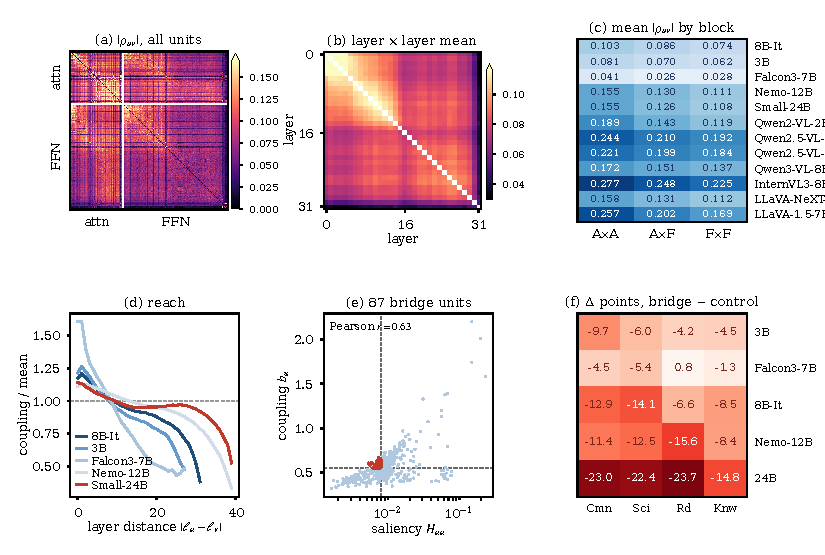
\includegraphics[width=0.97\textwidth]{cocurve_edge_anatomy.pdf}
\caption{Structure carried by the co-pruning curvature matrix. The panels expose cross-module and long-range coupling, identify low-saliency/high-coupling bridge units, and test those bridge units against matched controls.}
\label{fig:cc-anatomy}
\end{figure}

Figure~\ref{fig:cc-lambda} shows that the interaction weight induces a finite, enumerable solution path rather than an unconstrained tuning axis.
\begin{figure}[tbp]
\centering
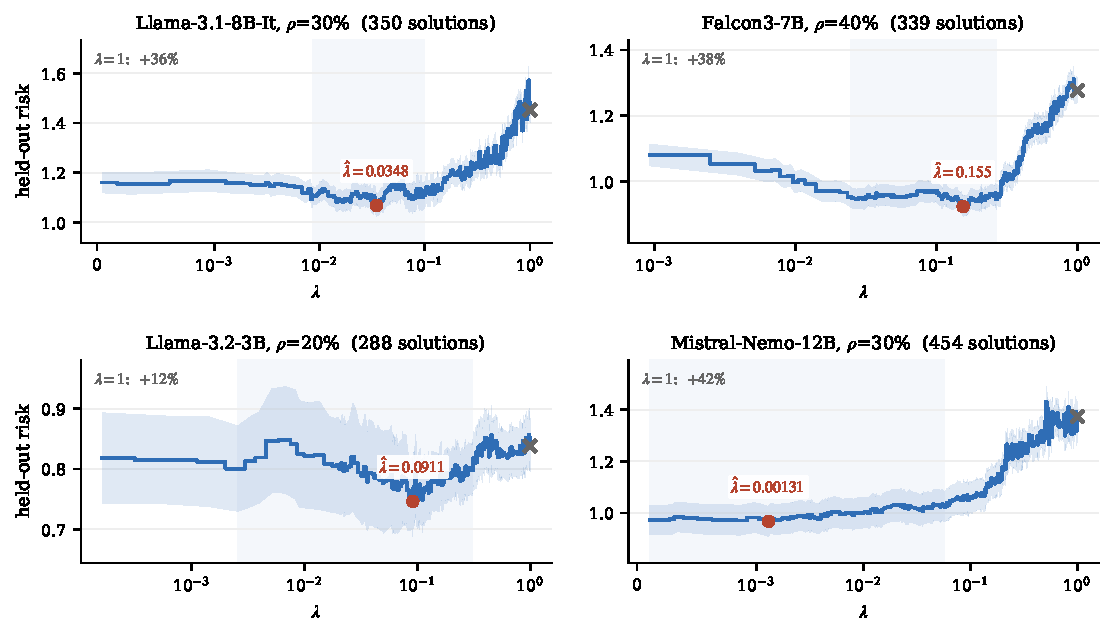
\includegraphics[width=0.78\textwidth]{cocurve_lambda_path.pdf}
\caption{Finite interaction-strength solution path. Ordering changes occur only at a finite set of breakpoints, allowing $\lambda$ to be calibrated by held-out KL on unlabeled text rather than task labels.}
\label{fig:cc-lambda}
\end{figure}

\subsubsection{What the matrix reveals mechanistically}
The matrix is not useful because it improves pruning. It exposes a model structure that node scores systematically discard. Normalizing an edge by
\begin{equation}
\rho_{uv}=\frac{H_{uv}}{\sqrt{H_{uu}H_{vv}}}
\label{eq:cc-corr}
\end{equation}
puts all interactions on one scale. Across five text models, the attention--FFN block is reported at 0.74--0.98$\times$ the mean within-module coupling, and coupling remains 0.33--0.53$\times$ the average even across the full depth. The matrix also identifies a small ``bridge'' population: low diagonal saliency but high total coupling $b_u=\sum_{v\neq u}|H_{uv}|$. On Llama-3.1-8B, 87 of 768 units lie in this corner. A diagonal selector removes them early; \CoCurve{} becomes increasingly reluctant to remove them as their partners disappear.

The paper tests this interpretation causally rather than relying on correlation. Bridge units are forcibly removed and compared against a control matched on saliency, unit type, and parameter cost. The bridge-removal arm loses capability in 19 of 20 model-by-domain cells, with losses up to 23.7 points. This is a concrete reason interaction-aware compression helps: the off-diagonal identifies low-saliency units whose \emph{position in the computation graph} makes them load-bearing.

\subsubsection{Evaluation: accuracy at a fixed physical budget}
All methods are evaluated after physically slicing structured weights, so the reported speedups are not masked-model FLOP proxies. At 20\% removal on Llama-3.1-8B-Instruct, \CoCurve{} gives WikiText perplexity 12.88 and C4 perplexity 19.58; Table~\ref{tab:cc-main} shows the corresponding capability results, while Figure~\ref{fig:cc-ratio} and Table~\ref{tab:cc-ratio-sweep} extend the comparison across removal ratios and model scales. The benefit persists over ratios and model scales rather than appearing at one operating point.

\begin{table}[tbp]
\centering\singlespacing\scriptsize
\caption{Llama-3.1-8B-Instruct at 20\% structured removal. Perplexity and downstream capability at 20\% structured removal. Lower is better for Wiki/PTB/C4; higher is better for the remaining tasks.}
\label{tab:cc-main}
\setlength{\tabcolsep}{2.1pt}
\begin{adjustbox}{max width=\textwidth}
\begin{tabular}{lrrrrrrrrrrrr}
\toprule
\textbf{Method} & \textbf{Wiki}$\downarrow$ & \textbf{PTB}$\downarrow$ & \textbf{C4}$\downarrow$ & \textbf{ARC-c} & \textbf{ARC-e} & \textbf{HellaS} & \textbf{WinoG} & \textbf{PIQA} & \textbf{OBQA} & \textbf{BoolQ} & \textbf{CS Avg.} & \textbf{MMLU}\\
\midrule
Dense (0\%) & 6.40 & 10.36 & 10.67 & .544 & .781 & .774 & .662 & .809 & .476 & .850 & .700 & .478\\
Random & 21.20 & 30.44 & 36.77 & .294 & .503 & .538 & .545 & .682 & .314 & .654 & .504 & .318\\
Magnitude & 20.49 & 31.38 & 34.93 & .314 & .546 & .555 & .559 & .689 & .324 & .652 & .520 & .328\\
Wanda-sp & 20.02 & 35.29 & 30.09 & .388 & .625 & .574 & .570 & .737 & .364 & .722 & .569 & .356\\
FLAP & 20.88 & 36.77 & 29.06 & .377 & .625 & .590 & .549 & .732 & .382 & .709 & .566 & .353\\
AMP & 20.39 & 47.27 & 33.26 & .388 & .639 & .581 & .567 & .747 & .388 & .694 & .572 & .357\\
LLM-Pruner & 13.23 & \textbf{19.36} & 21.98 & .372 & .604 & .646 & .574 & .750 & .368 & \textbf{.791} & .586 & .368\\
SlimGPT & 19.24 & 35.52 & 29.19 & .374 & .619 & .588 & .566 & .734 & .354 & .643 & .554 & .351\\
SlimLLM & 17.36 & 30.59 & 29.36 & .395 & .652 & .600 & .562 & .752 & .398 & .658 & .574 & .372\\
2SSP & 16.29 & 24.07 & 29.00 & .413 & \textbf{.668} & .619 & .597 & .736 & .386 & .643 & .580 & .379\\
\textbf{\CoCurve{}} & \textbf{12.88} & 29.63 & \textbf{19.58} & \textbf{.419} & .625 & \textbf{.675} & \textbf{.610} & \textbf{.758} & .396 & .783 & \textbf{.609} & \textbf{.385}\\
\bottomrule
\end{tabular}
\end{adjustbox}
\end{table}

\begin{figure}[tbp]
\centering
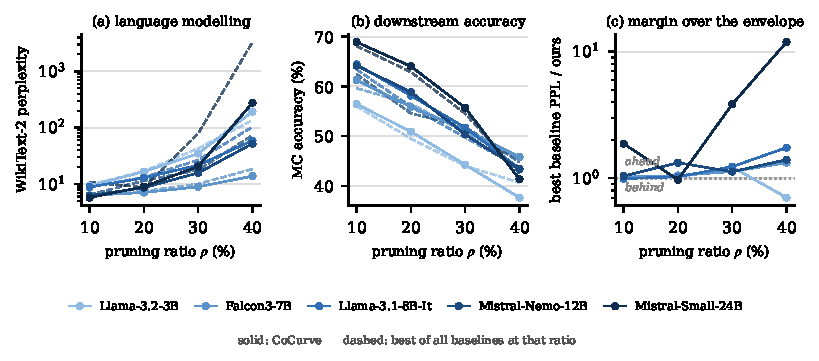
\includegraphics[width=0.94\textwidth]{cocurve_ratio_full.pdf}
\caption{Performance across removal ratios and text-model scales. Solid curves are \CoCurve{}; dashed curves form the best-baseline envelope at each ratio, showing that the advantage persists across operating points rather than one chosen budget.}
\label{fig:cc-ratio}
\end{figure}

\begin{table}[tbp]
\centering\singlespacing\scriptsize
\caption{Performance across structured-removal ratios on five text models. Each cell reports C4 perplexity $\downarrow$ / commonsense mean accuracy $\uparrow$. ``Best baseline'' is the strongest of the seven training-free baselines at that ratio, so it is an envelope rather than one fixed competitor.}
\label{tab:cc-ratio-sweep}
\setlength{\tabcolsep}{4.0pt}\renewcommand{\arraystretch}{1.04}
\begin{tabular}{llrrrrr}
\toprule
\textbf{Model} & \textbf{Selector} & \textbf{10\%} & \textbf{20\%} & \textbf{30\%} & \textbf{40\%} & \textbf{50\%}\\
\midrule
Llama-3.2-3B & Best baseline & 9.6/56 & 16.9/50 & 42.7/44 & \textbf{136/41} & \textbf{1199/37}\\
\rowcolor{SoftBlue}& \textbf{\CoCurve{}} & \textbf{9.3/56} & \textbf{16.7/51} & \textbf{34.8/44} & 194/38 & 4617/35\\
\addlinespace[1pt]
Falcon3-7B & Best baseline & 6.4/60 & 7.4/\textbf{56} & 10.1/51 & 18.4/45 & 42.6/39\\
\rowcolor{SoftBlue}& \textbf{\CoCurve{}} & \textbf{6.3/61} & \textbf{7.1/56} & \textbf{8.9/51} & \textbf{13.8/46} & \textbf{41.7/40}\\
\addlinespace[1pt]
Llama-3.1-8B-It & Best baseline & \textbf{8.8}/63 & 13.2/56 & 26.6/50 & 103/\textbf{44} & \textbf{773}/37\\
\rowcolor{SoftBlue}& \textbf{\CoCurve{}} & 8.9/\textbf{64} & \textbf{12.9/58} & \textbf{21.6/52} & \textbf{59.1}/43 & 956/\textbf{38}\\
\addlinespace[1pt]
Mistral-Nemo-12B & Best baseline & 6.5/62 & 11.4/55 & 17.8/\textbf{52} & 73.1/\textbf{45} & \textbf{513/40}\\
\rowcolor{SoftBlue}& \textbf{\CoCurve{}} & \textbf{6.2/64} & \textbf{8.6/59} & \textbf{15.8}/50 & \textbf{52.2}/43 & 839/38\\
\addlinespace[1pt]
Mistral-Small-24B & Best baseline & 10.8/68 & \textbf{8.7}/63 & 78.8/55 & 3299/\textbf{43} & 4666/35\\
\rowcolor{SoftBlue}& \textbf{\CoCurve{}} & \textbf{5.7/69} & 9.0/\textbf{64} & \textbf{20.5/56} & \textbf{277}/41 & \textbf{2560/36}\\
\bottomrule
\end{tabular}
\end{table}


\begin{table}[tbp]
\centering\singlespacing\footnotesize
\caption{Vision-language transfer at two structured-removal ratios (seven-benchmark mean accuracy, \%). The diagonal-only row uses the same estimator and budget protocol but removes all off-diagonal interactions, isolating the contribution of coupling.}
\label{tab:cc-vlm-sweep}
\setlength{\tabcolsep}{5pt}\renewcommand{\arraystretch}{1.05}
\begin{tabular}{lrrrr}
\toprule
& \multicolumn{2}{c}{\textbf{Qwen2.5-VL-7B}} & \multicolumn{2}{c}{\textbf{Qwen3-VL-8B}}\\
\cmidrule(lr){2-3}\cmidrule(lr){4-5}
\textbf{Selector} & \textbf{20\%} & \textbf{30\%} & \textbf{20\%} & \textbf{30\%}\\
\midrule
Dense (no pruning) & 81.6 & 81.6 & 83.4 & 83.4\\
\rowcolor{SoftBlue}\textbf{\CoCurve{}} & \textbf{74.4} & \textbf{63.6} & \textbf{71.1} & \textbf{57.7}\\
Diagonal only ($\lambda=0$) & 73.5 & 61.1 & 66.5 & 50.1\\
\midrule
LLM-Pruner & 72.2 & 57.2 & 65.8 & 47.0\\
Wanda-sp & 62.9 & 52.2 & 40.5 & 35.9\\
FLAP & 73.3 & 58.5 & 68.4 & 46.5\\
ShortGPT (layer drop) & 35.3 & 35.2 & 35.2 & 35.3\\
Magnitude & 72.9 & 58.7 & 57.0 & 37.7\\
Random & 64.4 & 46.2 & 53.8 & 41.2\\
\bottomrule
\end{tabular}
\end{table}


Table~\ref{tab:cc-vlm-sweep} tests the same interaction-aware selector on vision--language models. The VLM sweep shows that the interaction term remains useful beyond decoder-only language models: on Qwen2.5-VL-7B and Qwen3-VL-8B, \CoCurve{} remains ahead of both diagonal-only selection and the listed structured baselines at 20\% and 30\% removal. The full study extends this comparison to five VLMs from three families, where \CoCurve{} leads the best baseline at 20\% removal on all five. This supports the broader claim that the estimated interaction object is not tied to one architecture family or one pruning ratio.

\textbf{Deployment efficiency.} \CoCurve{} exports physically sliced dense submodels, so the resource claim is measured on the model that is actually executed rather than on a masked full-size network. Table~\ref{tab:cc-efficiency} shows the resulting parameter, latency, and peak-memory changes. At 40\% removal, Llama-3.2-3B and Llama-3.1-8B-Instruct reach 1.40$\times$ and 1.49$\times$ prefill speedup while using about 0.66$\times$ peak memory.

\begin{table}[t]
\centering\singlespacing\footnotesize
\caption{Measured efficiency after physical structured removal. Parameter and peak-memory values are ratios to the dense model (lower is better); prefill/decode values are speedups (higher is better).}
\label{tab:cc-efficiency}
\setlength{\tabcolsep}{6pt}
\begin{tabular}{lrrrrr}
\toprule
\textbf{Model} & \textbf{Removed} & \textbf{Params}$\downarrow$ & \textbf{Prefill}$\uparrow$ & \textbf{Decode}$\uparrow$ & \textbf{Peak mem.}$\downarrow$\\
\midrule
Llama-3.2-3B & 20\% & 0.82$\times$ & 1.17$\times$ & 1.10$\times$ & 0.83$\times$\\
Falcon3-7B & 20\% & 0.82$\times$ & 1.19$\times$ & 1.16$\times$ & 0.83$\times$\\
Llama-3.1-8B-Instruct & 20\% & 0.83$\times$ & 1.17$\times$ & 1.06$\times$ & 0.83$\times$\\
Mistral-Nemo-12B & 20\% & 0.82$\times$ & 1.21$\times$ & 1.18$\times$ & 0.82$\times$\\
\midrule
Llama-3.2-3B & 40\% & 0.65$\times$ & 1.40$\times$ & 1.09$\times$ & 0.66$\times$\\
Llama-3.1-8B-Instruct & 40\% & 0.65$\times$ & 1.49$\times$ & 1.22$\times$ & 0.66$\times$\\
Mistral-Small-24B & 40\% & 0.62$\times$ & -- & -- & 0.63$\times$\\
\bottomrule
\end{tabular}
\end{table}

The point is not a new sparse kernel: because methods at a fixed removed fraction execute similarly sized dense submodels, the main contribution is selecting a substantially better model at the same physical budget.

\begin{insightbox}
\textbf{What \CoCurve{} adds to the thesis.} \SubspacePath{} made execution conditional on \emph{where the model is deployed}; \CoCurve{} makes execution conditional on \emph{what else has already been removed}. The technical move is from scalar importance to an interaction matrix that is still practical to estimate. This is the model-execution counterpart of the internal non-separability exposed earlier by \CoAx{}.
\end{insightbox}

\subsection{High-Sparsity Structured Compression with \AnchorPath{} \texorpdfstring{\projecticon{https://gongzhiren.github.io/AnchorPath-website/}}{}}
\label{sec:anchor}

\textbf{Pushing the pruning boundary.} Interaction-aware selection improves which units are removed, but a separate challenge appears as the structured pruning ratio becomes high. After many units have already been removed, the remaining model is no longer close to the dense checkpoint on which a one-shot criterion was estimated; continuing to trust that unchanged surrogate can therefore produce rapidly compounding errors. \AnchorPath{} targets this high-sparsity regime directly: it keeps the dense model as a stable reference while periodically refreshing the local selection signal around the current pruned model~\citep{gong2026anchorpath}. The goal is deployment-oriented---push the usable pruning ratio farther while preserving capability.

Figure~\ref{fig:anchor-method} contrasts one-shot extrapolation with the anchored continuation used at high pruning ratios.
\begin{figure}[tbp]
\centering
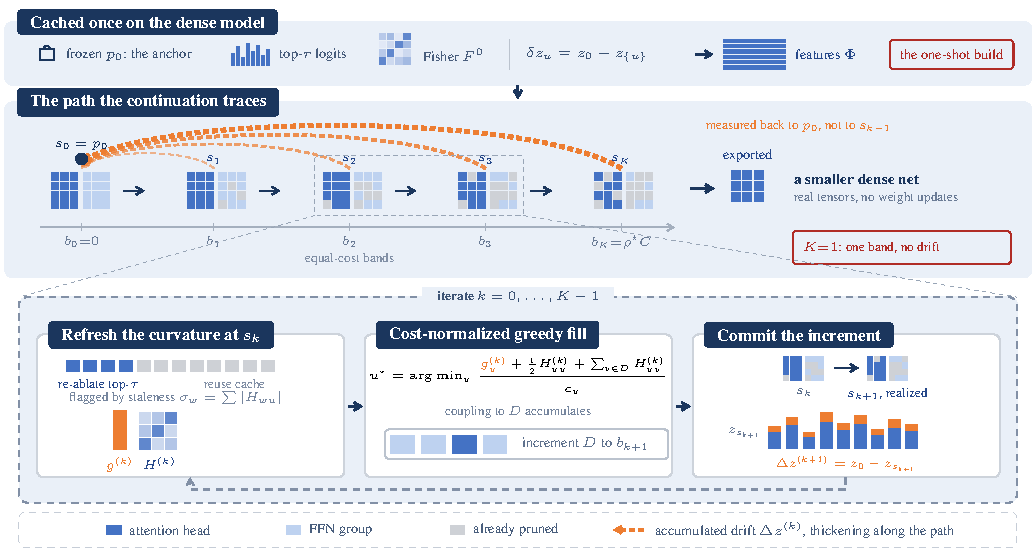
\includegraphics[width=0.90\textwidth]{anchor_overview_full.pdf}
\caption{\AnchorPath{} conceptual comparison. One-shot extrapolates a dense-point quadratic over the entire budget; anchored continuation moves the expansion point along a nested pruning path while keeping the dense teacher fixed~\citep{gong2026anchorpath}.}
\label{fig:anchor-method}
\end{figure}

\subsubsection{Anchored continuation}
Let $s_k$ be the removal state after step $k$, and keep the dense teacher $p_0$ fixed as a global anchor. At the current pruned model, a surviving unit $u$ has marginal logit perturbation $\delta z_u^{(k)}$ and accumulated drift $\Delta z^{(k)}=z_0-z_{s_k}$. Using the dense Fisher metric $F^0$, the refreshed local surrogate contains
\begin{align}
g_u^{(k)}&=\mathbb E\!\left[\Delta z^{(k)\top}F^0\delta z_u^{(k)}\right],\label{eq:ap-grad}\\
H_{uv}^{(k)}&=\mathbb E\!\left[\delta z_u^{(k)\top}F^0\delta z_v^{(k)}\right].\label{eq:ap-hess}
\end{align}
The next unit is chosen by a cost-normalized local marginal
\begin{equation}
\Delta(u\mid D)=\frac{g_u^{(k)}+\tfrac12H_{uu}^{(k)}+\sum_{v\in D}H_{uv}^{(k)}}{c_u}.
\label{eq:ap-marginal}
\end{equation}
At $k=0$, $\Delta z^{(0)}=0$ so the drift term vanishes: a single-step run reduces exactly to one-shot second-order pruning. Multi-step continuation therefore changes only one thing---\textbf{the surrogate is periodically rebuilt along the compression path}.


A step-splitting analysis bounds ideal Taylor remainder by an $O(1/K^2)$ term plus surrogate-mismatch error, explaining why smaller moves remain nearer their local trust region. To avoid $K$ full rebuilds, the method uses the already estimated interaction matrix as a staleness detector and refreshes only the surviving units most strongly coupled to what has recently been removed.

\begin{table}[H]
\centering\singlespacing\small
\caption{Headline degradation curve on LLaMA-3.1-8B (WikiText-2 perplexity $\downarrow$, calibration-only, no recovery). The widening gap shows how rapidly a dense-point surrogate becomes unreliable as the operating point moves farther from dense.}
\label{tab:anchor-main}
\begin{tabular}{lrrrr}
\toprule
\textbf{Method} & $\rho=0.2$ & $\rho=0.3$ & $\rho=0.4$ & $\rho=0.5$\\
\midrule
LLM-Pruner & 14.5 & 30.0 & 103.3 & 718.2\\
One-shot ($K=1$) & 14.0 & 33.0 & 245.9 & 4106\\
\textbf{\AnchorPath{} ($K=8$)} & \textbf{12.1} & \textbf{23.2} & \textbf{47.2} & \textbf{245}\\
\midrule
Gain vs. one-shot & 1.2$\times$ & 1.4$\times$ & 5.2$\times$ & 16.8$\times$\\
\bottomrule
\end{tabular}
\end{table}

Table~\ref{tab:anchor-main} shows the widening one-shot degradation as sparsity increases. Across seven reported model families, the same conservative $K=8$ equal-cost configuration improves over one-shot in every model/ratio cell. Because the final mask is exported to the same structured budget, deployment-time parameters/FLOPs/latency are unchanged relative to a one-shot mask at that ratio; only calibration-time selection is more expensive.

\begin{insightbox}
\AnchorPath{} marks the boundary of static pruning as a paradigm: even a good interaction model becomes stale when a large sequence of removals moves the operating point. It therefore completes Part~I's progression from \emph{context-conditioned ranking} to \emph{interaction-aware set selection} to \emph{state-aware continuation}.
\end{insightbox}

\subsection{Part I synthesis}
The three projects address progressively harder deployment regimes while keeping one objective fixed: reduce executed backbone cost without discarding the capacity needed by the current condition.

\begin{tcbraster}[raster columns=3,raster equal height=rows,raster column skip=5pt]
\begin{tcolorbox}[colback=SoftBlue!55,colframe=NTUblue!55,boxrule=.45pt,arc=1.5pt]
\textbf{1. Scenario specialization}\\[-1mm]
\SubspacePath{} \projecticon{https://gongzhiren.github.io/SubspacePathPruner-website/}\\
\small\raggedright Read the deployment scenario and compile a reusable head pathway without scenario-specific training.
\end{tcolorbox}
\begin{tcolorbox}[colback=SoftBlue!40,colframe=NTUblue!55,boxrule=.45pt,arc=1.5pt]
\textbf{2. Model-wide compression}\\[-1mm]
\CoCurve{} \projecticon{https://gongzhiren.github.io/CoCurve-website/}\\
\small\raggedright Remove structured redundancy under one budget while accounting for interactions across attention and FFN units.
\end{tcolorbox}
\begin{tcolorbox}[colback=SoftBlue!28,colframe=NTUblue!55,boxrule=.45pt,arc=1.5pt]
\textbf{3. Higher sparsity}\\[-1mm]
\AnchorPath{} \projecticon{https://gongzhiren.github.io/AnchorPath-website/}\\
\small\raggedright Refresh the selection signal as pruning changes the remaining model, preserving quality at more aggressive ratios.
\end{tcolorbox}
\end{tcbraster}

\begin{transitionbox}
\textbf{Part I takeaway.} The model-side problem changes as deployment becomes more demanding: first identify the scenario-specific capacity to retain, then account for interactions in model-wide compression, and finally keep the selection signal valid as structured sparsity increases.
\end{transitionbox}

\clearpage
% ======================================================================
\section{Part II: Adaptive Reasoning}
\label{sec:reasoning}

Part~II addresses the external/test-time side of the same deployment problem. A compressed or specialized model is still asked to reason under heterogeneous demand. The control variable therefore moves from model/scenario scale to reasoning-step scale: first decide \emph{what evidence and how much reasoning} the current state needs, then decide \emph{which internal pathway} should execute that step.

\begin{transitionbox}
\textbf{Part II question.} After the model is deployed, can reasoning computation itself follow the current state of the problem---selecting the evidence, depth, and internal pathway needed \emph{now}---instead of executing one externally prescribed procedure everywhere?
\end{transitionbox}

\paragraph{Reasoning-side motivation.} \XDB{}\workref{D1}{sec:xdb} shows that capable models can still struggle when several knowledge domains must be composed, and that the reasoning demand changes further as an interaction unfolds. Existing test-time methods usually respond by prescribing an external procedure---a chain, a plan, a revision loop, sampling, search, or a memory rule. The open allocation question is therefore simple to state: \emph{how should the reasoning process adapt when the current problem or the current step needs different evidence and different amounts of computation?} Part~II addresses this question first at the trajectory level with \SoT{} (Section~\ref{sec:sot}) and then inside each reasoning step with \LoTR{} (Section~\ref{sec:lotr}).

\subsection{Endogenous Reasoning Control with \SoT{} \texorpdfstring{\projecticon{https://gongzhiren.github.io/SoT-website/}}{}}
\label{sec:sot}

\textbf{Problem and idea.} Reasoning problems vary in difficulty, relevant evidence, and the point at which additional computation stops being useful. A fixed test-time recipe can therefore over-compute on easy cases yet still organize evidence poorly on harder or longer trajectories. \SoT{} asks whether the \emph{model's own evolving state} can supply a compact feedback signal for these decisions. The backbone stays frozen; the controller reads a sentence-level endogenous state, uses it to select useful history, and stops when the state indicates that further reasoning is no longer warranted~\citep{gong2026sot}.

Figure~\ref{fig:sot-overview} provides the high-level closed-loop view before the state and operators are defined.
\begin{figure}[tbp]
\centering
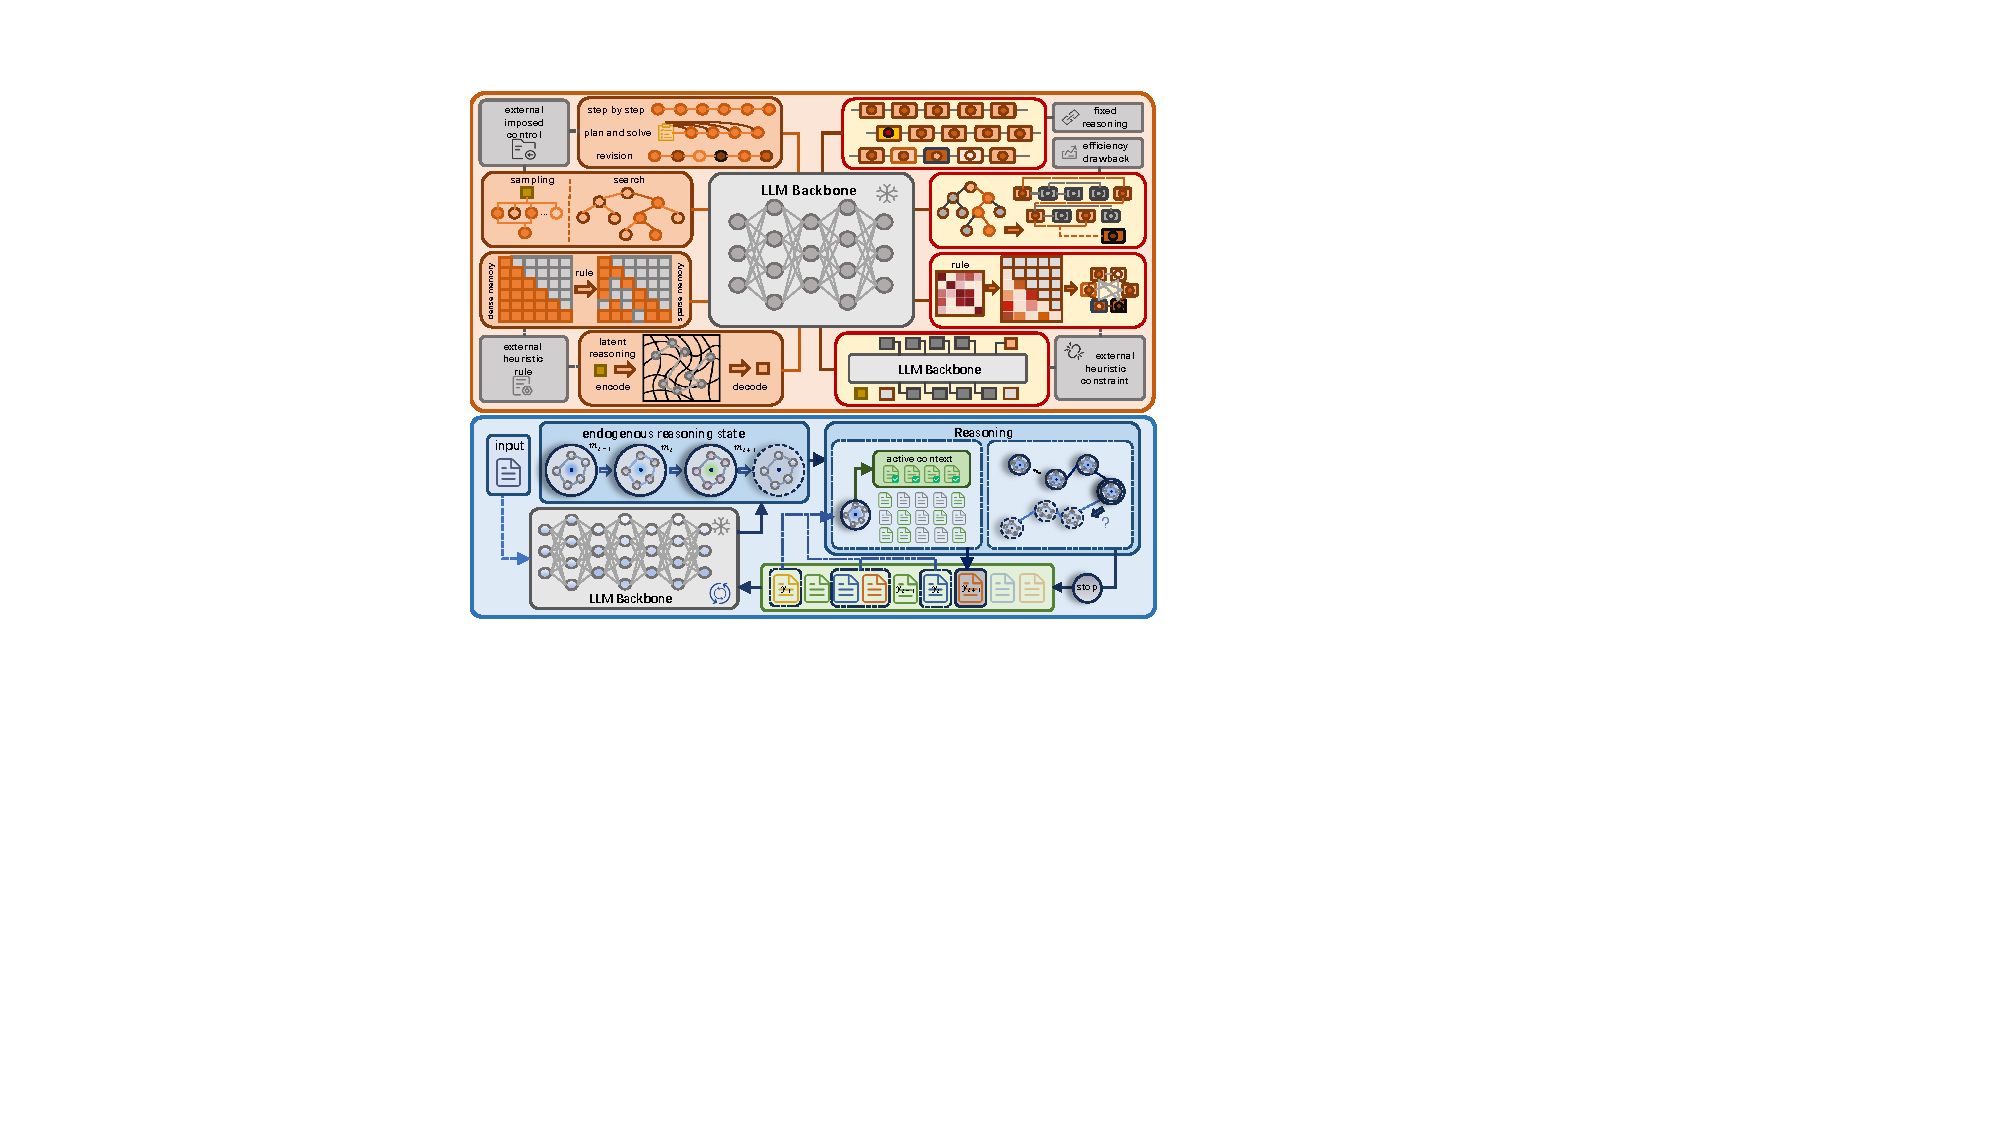
\includegraphics[width=0.94\textwidth]{sot_intro_main.pdf}
\caption{From externally prescribed reasoning to an endogenous closed loop. Conventional strategies determine the procedure outside the model; \SoT{} reads the model's evolving state and uses it to control the reasoning trajectory.}
\label{fig:sot-overview}
\end{figure}

\subsubsection{Reasoning as a closed-loop policy}
For frozen autoregressive model $f$, a reasoning policy $\pi$ generates trajectory $y_{1:T}$ and answer $a$:
\begin{equation}
\mathbb P_{\pi}(a,y_{1:T}\mid p)=
\prod_{t=1}^{T}\mathbb P_{\pi}(y_t\mid p,y_{<t})\,
\mathbb P_{\pi}(a\mid p,y_{1:T}).
\label{eq:sot-trajectory}
\end{equation}
Conventional paradigms mainly change the external policy class. \SoT{} instead reads a compact endogenous state from each sentence-level reasoning unit. Let $h^{(L)}_{t,i}\in\mathbb R^D$ be the final-layer hidden state of token $i$ in sentence $y_t$, let $n_t$ be its length, and define the sentence center $u_t=n_t^{-1}\sum_i h^{(L)}_{t,i}$. The raw state is
\begin{equation}
s_t=[\delta_t,\ v_t,\ c_t,\ H_t]^\top,
\qquad
m_t=\frac{s_t-\mu}{\sigma+\varepsilon}\in\mathbb R^4,
\label{eq:sot-state}
\end{equation}
with componentwise offline mean $\mu$ and standard deviation $\sigma$. Its four coordinates are
\begin{align}
\delta_t&=\frac1{n_t}\sum_i\|h^{(L)}_{t,i}\|_2^2-\|u_t\|_2^2, &
v_t&=\|u_t-u_{t-1}\|_2, \label{eq:sot-state-components}\\
c_t&=\frac{\langle u_t-u_{t-1},\,u_{t-1}-u_{t-2}\rangle}
{\|u_t-u_{t-1}\|_2\|u_{t-1}-u_{t-2}\|_2+\varepsilon}, &
H_t&=\frac1{n_t}\sum_i\mathcal H(p_{t,i}), \nonumber
\end{align}
where $\mathcal H$ is Shannon entropy and $p_{t,i}$ is the next-token predictive distribution at position $i$. Thus $\delta_t$ measures within-sentence dispersion, $v_t$ state movement, $c_t$ directional consistency, and $H_t$ local predictive uncertainty. The controller sees only this normalized four-dimensional interface, not the full hidden tensor.

Figure~\ref{fig:sot-state} shows that the four-dimensional state organizes trajectories from different reasoning paradigms into distinguishable dynamical regions.
\begin{figure}[tbp]
\centering
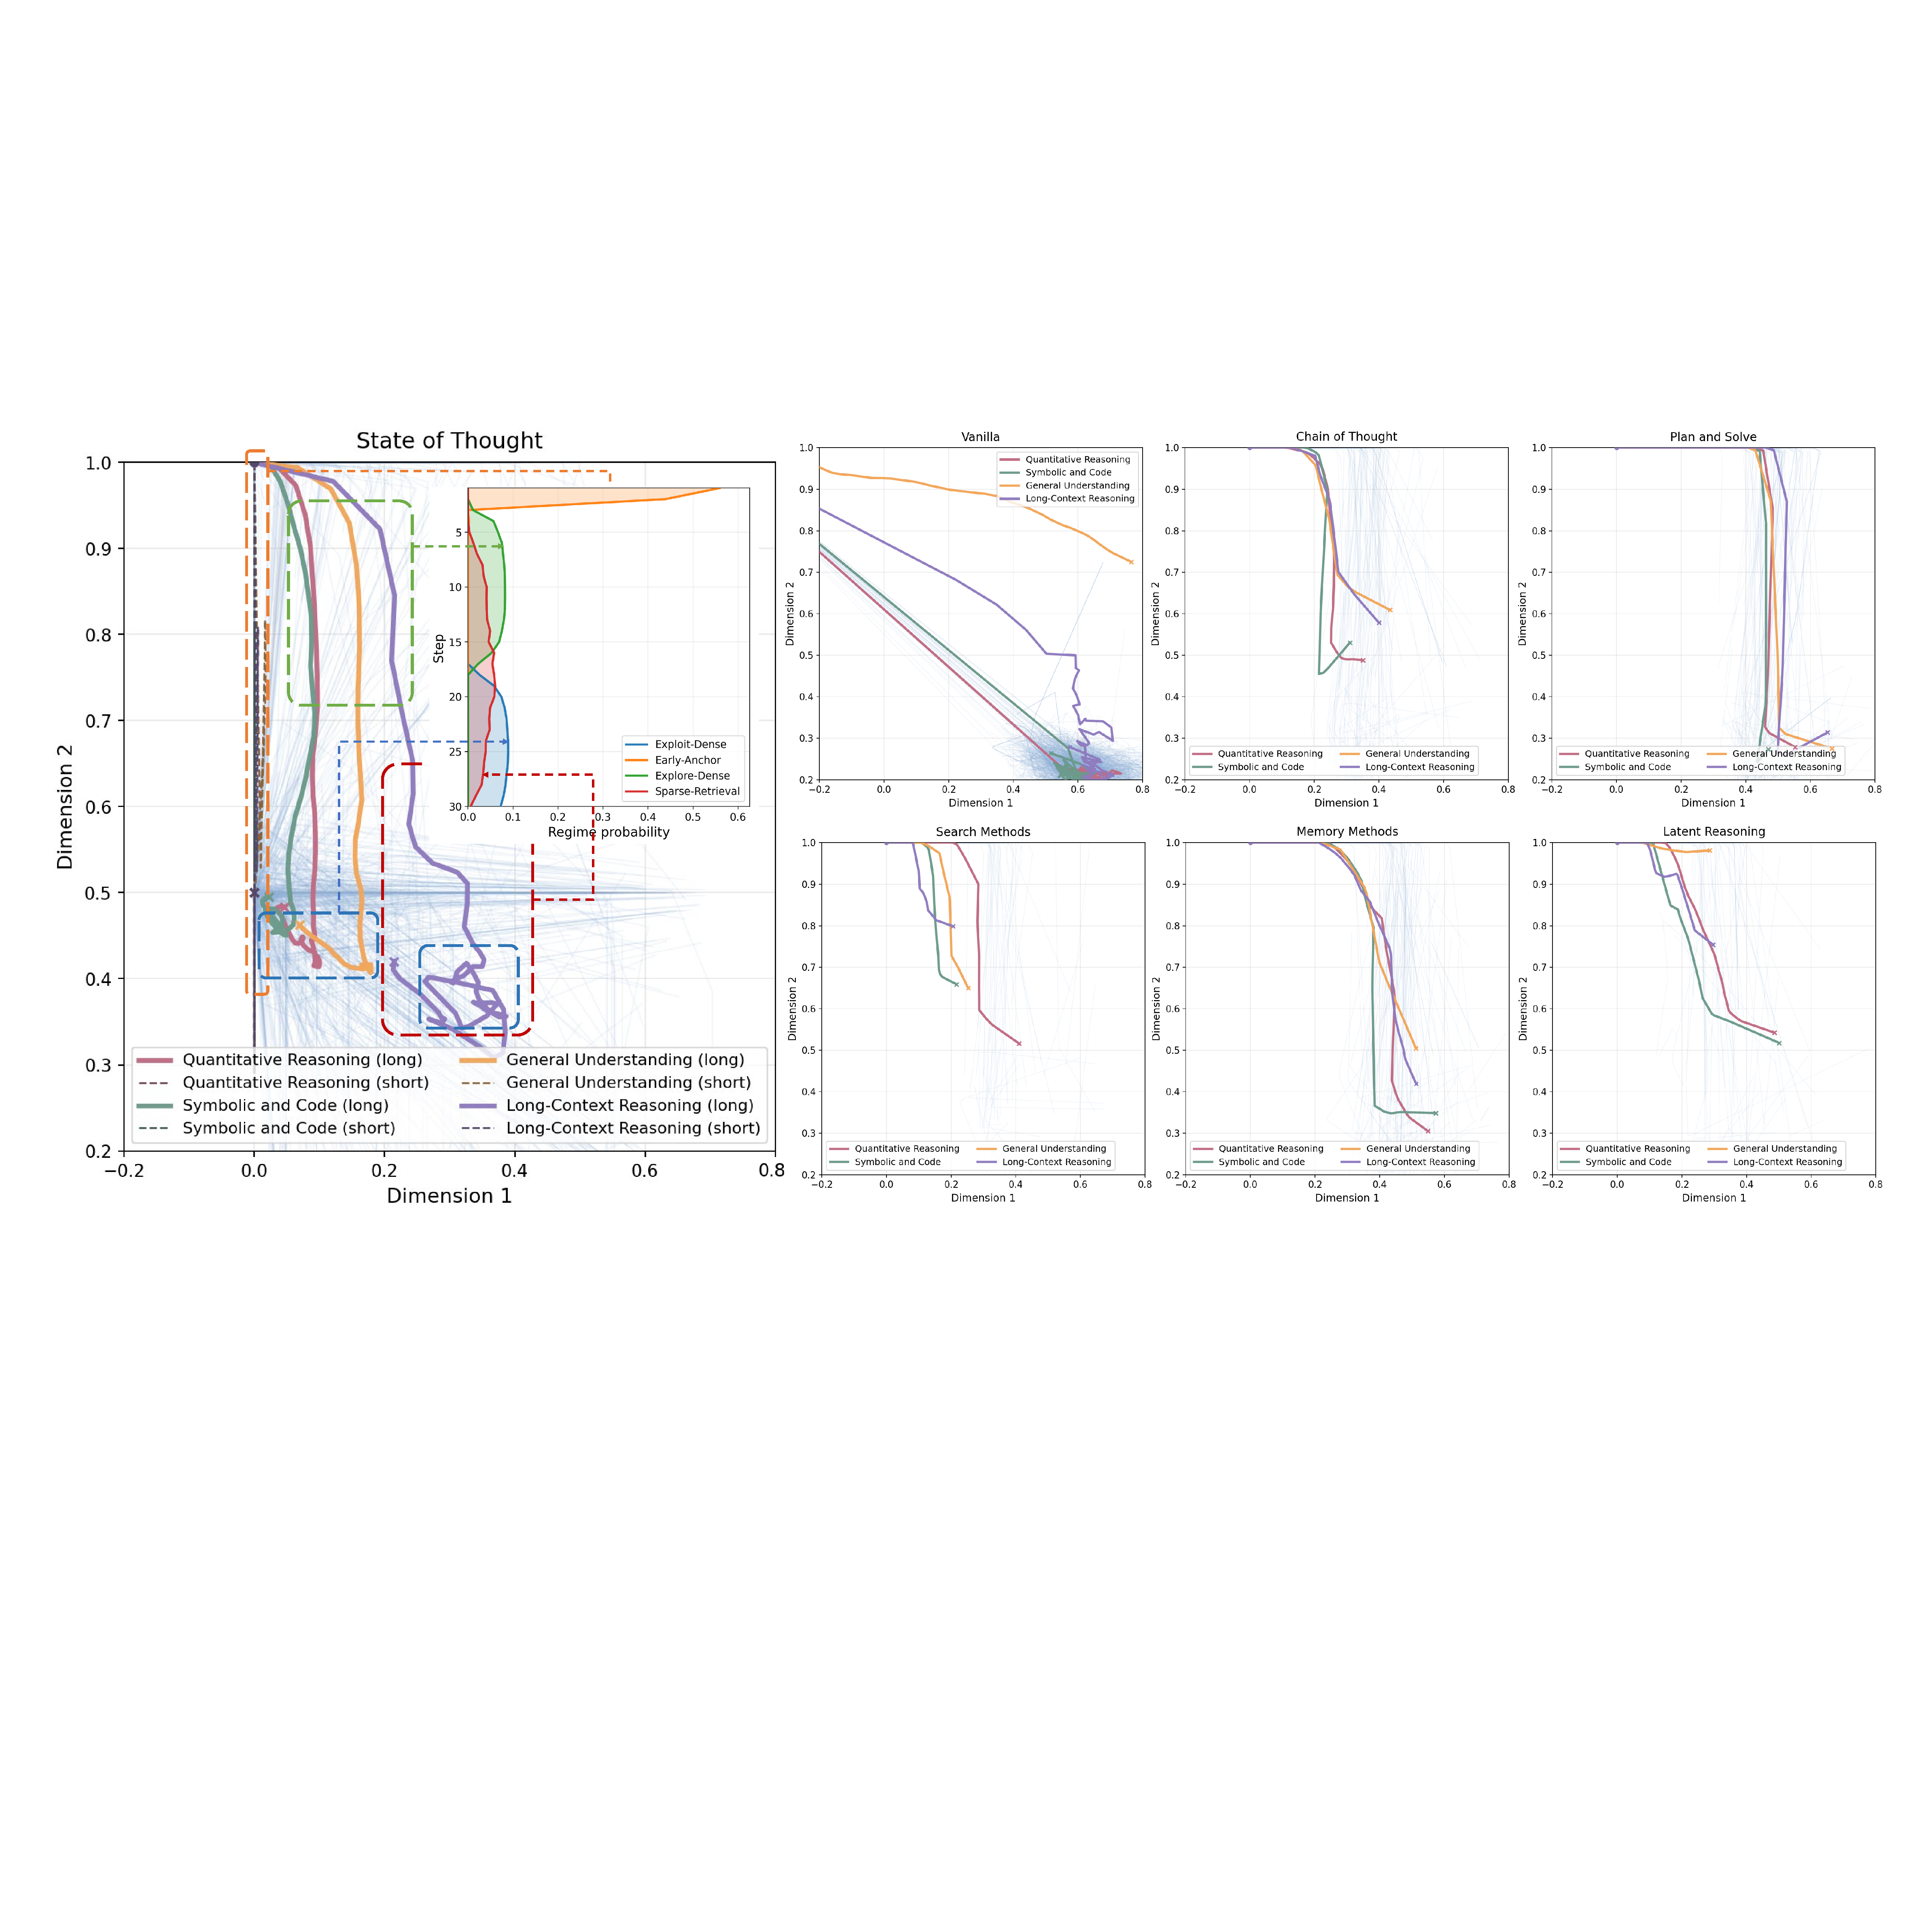
\includegraphics[width=0.93\textwidth]{sot_state_space_full.pdf}
\caption{Endogenous-state trajectories on Llama-3.1-8B. Different externally imposed paradigms occupy distinguishable regions of the dynamics--geometry state space, motivating a controller that reads this state directly~\citep{gong2026sot}.}
\label{fig:sot-state}
\end{figure}

\subsubsection{Two state-conditioned operators: evidence and stopping}
\SoT{} closes the loop with two lightweight operators. The evidence operator $\mathcal S$ chooses a sparse subset of history appropriate for the current state,
\begin{equation}
\widetilde y_{<t}=\mathcal S(y_{<t};m_t),\qquad
\mathbb P_{\pi}(y_t\mid p,y_{<t})=
\mathbb P(y_t\mid p,\widetilde y_{<t}),
\label{eq:sot-select}
\end{equation}
while the stopping operator $\mathcal T$ produces $z_t=\mathcal T(m_t)\in\{0,1\}$. If $z_t=1$, answer generation is triggered from the state-evidence and current step. The same state therefore controls \emph{what history remains active} and \emph{whether more computation is useful}.

Only $\mathcal S$ and $\mathcal T$ are trained; the backbone remains frozen. Offline multi-step trajectories provide preference-style supervision for useful historical evidence and stop proxies for whether further reasoning is warranted. This is deliberately a small control interface: the method does not fine-tune the model into one reasoning style.

Figure~\ref{fig:sot-activation} connects those state regions to the two control actions: sparse history selection and stopping.
\begin{figure}[tbp]
\centering
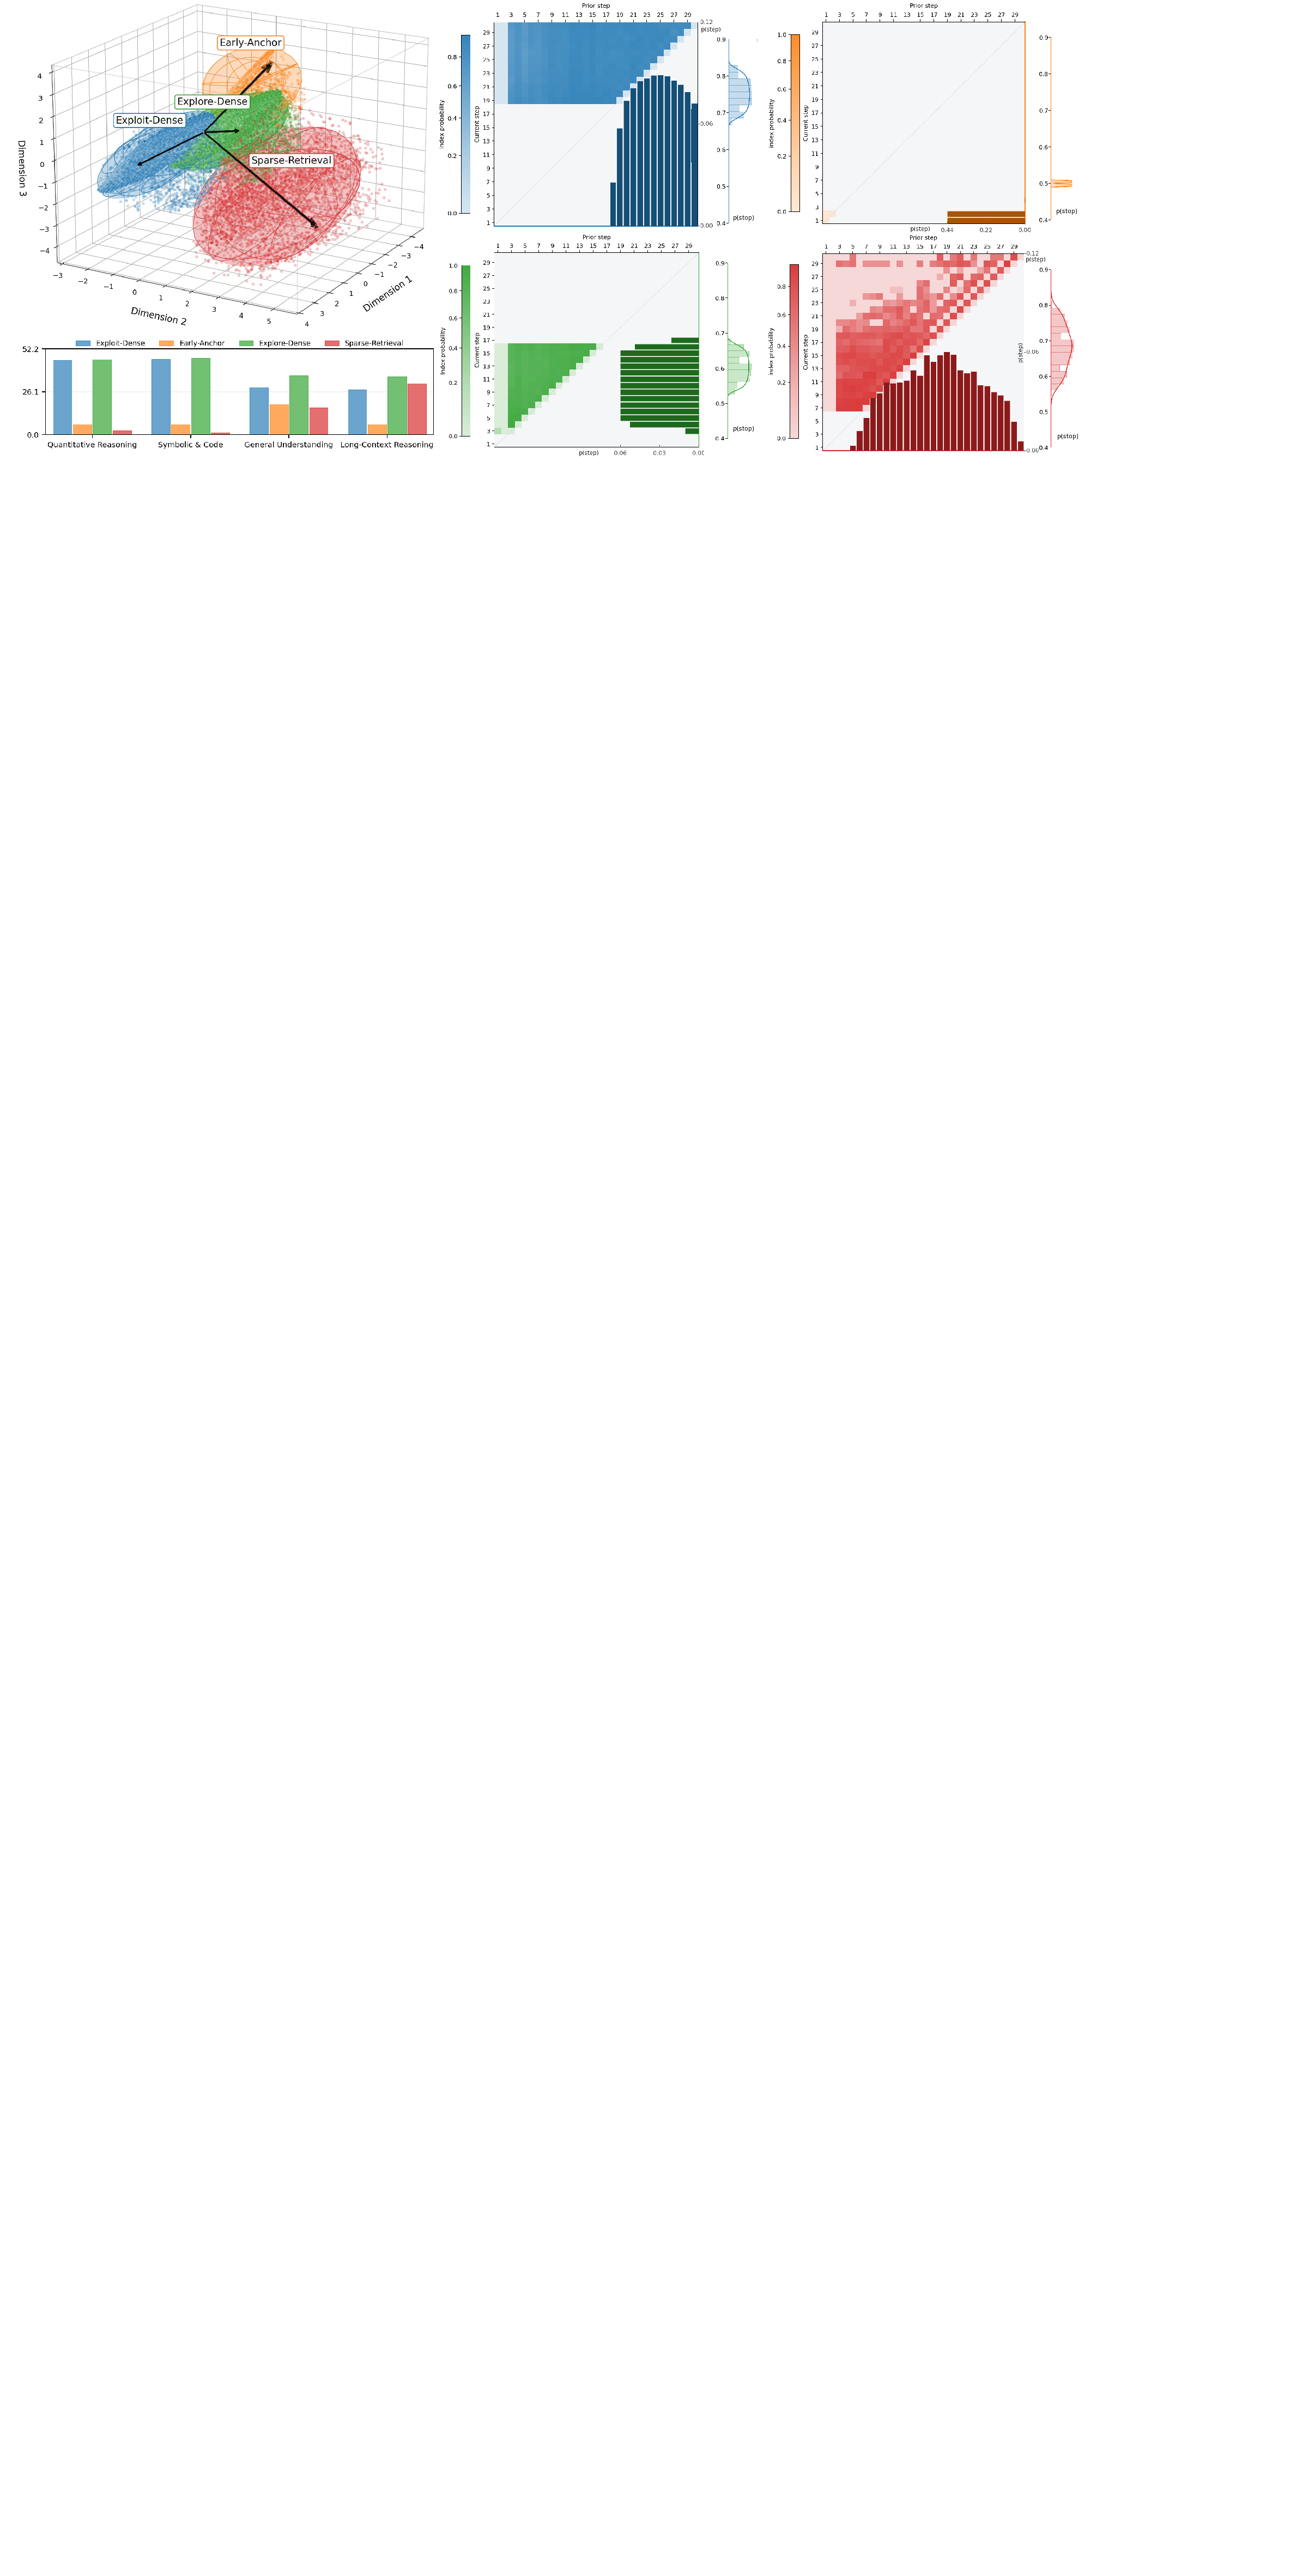
\includegraphics[width=0.94\textwidth]{sot_state_conditioned_full.pdf}
\caption{State-conditioned activation analysis. Distinct endogenous state clusters induce different sparse history-selection patterns and different stopping tendencies, providing an interpretable link from $m_t$ to the two control actions~\citep{gong2026sot}.}
\label{fig:sot-activation}
\end{figure}

\subsubsection{Evaluation protocol and main result}
The evaluation spans four frozen backbones (three LLMs and one VLM) and twenty datasets. For LLMs, the main suite is organized into Quantitative Reasoning, Symbolic/Code, General Understanding, and Long-Context Reasoning; the transfer suite adds four multimodal benchmarks. The comparison includes scripted reasoning, sampling/search, memory-oriented, latent-reasoning, and RL-based baselines under matched backbone access.

Figure~\ref{fig:sot-headline} summarizes the resulting quality--token--latency trade-off before the full task table.
\begin{figure}[tbp]
\centering
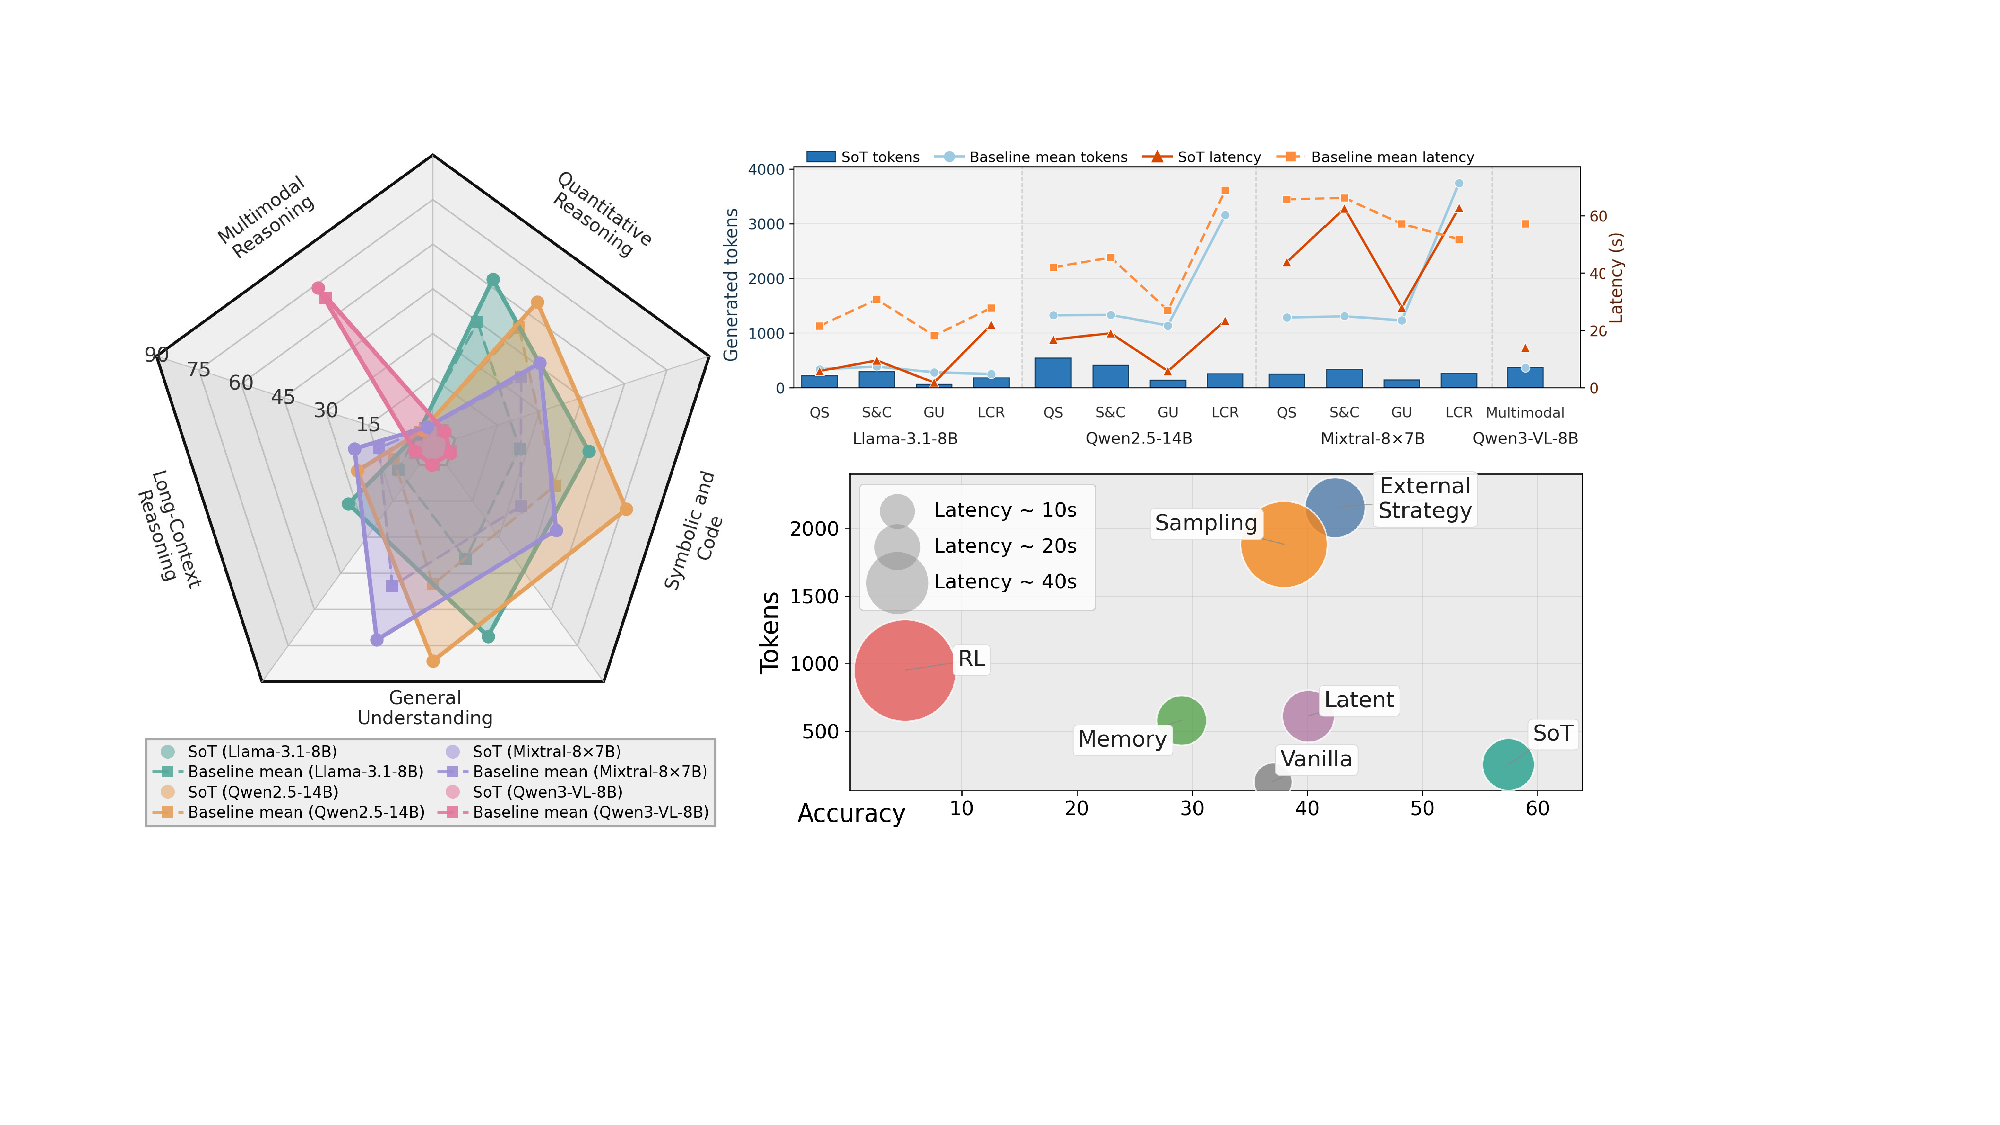
\includegraphics[width=0.93\textwidth]{sot_intro_overview.pdf}
\caption{\SoT{} at a glance: cross-domain quality, generated-token/latency cost, and the accuracy--efficiency frontier. The same endogenous-state controller is evaluated across heterogeneous reasoning regimes.}
\label{fig:sot-headline}
\end{figure}

The reported evaluation deliberately spans heterogeneous reasoning structures: quantitative reasoning, symbolic/code, general understanding, and long-context reasoning, over four backbones including a VLM. Baselines cover direct generation, seven externally scripted reasoning paradigms, sampling/search, memory-oriented methods, latent reasoning, and an RL-based method. Quality is reported with task-standard accuracy/F1/Pass@1; compute is measured by generated tokens and end-to-end latency.

Table~\ref{tab:sot-main-full} reports the complete Llama-3.1-8B benchmark matrix used for the main comparison.
\begin{table}[tbp]
    \centering
    \caption{Main results of \SoT{} on Llama-3.1-8B (accuracy, \%). The table spans quantitative, symbolic/code, general-understanding, and long-context reasoning and compares external reasoning, memory-oriented, latent, and RL-based alternatives under one evaluation harness.}
    \vspace{-2mm}
    \label{tab:sot-main-full}
    \footnotesize
    {\setlength{\tabcolsep}{1.85pt}%
     \setlength{\aboverulesep}{0pt}%
     \setlength{\belowrulesep}{0pt}%
     \setlength{\extrarowheight}{0pt}%
     \renewcommand{\arraystretch}{1.06}%
     \renewcommand{\tabularxcolumn}[1]{m{#1}}%
    \begin{tabularx}{\linewidth}{@{} >{\centering\arraybackslash}p{1.65cm} >{\centering\arraybackslash}m{1.38cm} !{\vrule width 0.4pt} >{\centering\arraybackslash}X >{\centering\arraybackslash}X >{\centering\arraybackslash}X >{\centering\arraybackslash}m{3.1em} >{\centering\arraybackslash}X >{\centering\arraybackslash}X >{\centering\arraybackslash}X >{\centering\arraybackslash}X >{\centering\arraybackslash}X >{\columncolor[HTML]{EAECEF}\centering\arraybackslash}m{3.1em} @{}}
    \toprule
    \multirow{2}{=}{\centering\textbf{Category}} & \multirow{2}{=}{\centering\textbf{Method}}
    & \multicolumn{4}{>{\cellcolor[HTML]{E3F2FD}}c!{\vrule width 1pt}}{\textbf{Quantitative Reasoning}}
    & \multicolumn{6}{>{\cellcolor[HTML]{E3F2FD}}c}{\textbf{Symbolic and Code}} \\
    &
    & {\scriptsize\textbf{GSM}} & {\scriptsize\textbf{MATH}} & {\scriptsize\textbf{DROP}} & \multicolumn{1}{>{\centering\arraybackslash}m{3.1em}!{\vrule width 1pt}}{\scriptsize\textbf{avg.}}
    & {\scriptsize\textbf{FOL}} & {\scriptsize\textbf{PW}} & {\scriptsize\textbf{BBH}} & {\scriptsize\textbf{HE}} & {\scriptsize\textbf{MBPP}} & \multicolumn{1}{>{\centering\arraybackslash}m{3.1em}}{\scriptsize\textbf{avg.}} \\
    \midrule
    Greedy & Vanilla & 79.0 & 58.2 & 6.2 & \multicolumn{1}{>{\centering\arraybackslash}m{3.1em}!{\vrule width 1pt}}{\cellcolor[HTML]{EAECEF}{53.9}} & 29.6 & 26.0 & 26.0 & 25.0 & \cellcolor[HTML]{FFD4D3}{55.2} & 33.0 \\
    \midrule
    \multirow{7}{=}{\centering Reasoning Paradigm}
    & CoT   & \cellcolor[HTML]{FFFCE0}{80.8} & \cellcolor[HTML]{FFD4D3}{64.2} & 1.7 & \multicolumn{1}{>{\centering\arraybackslash}m{3.1em}!{\vrule width 1pt}}{\cellcolor[HTML]{EAECEF}{55.5}} & 4.9 & 24.5 & \cellcolor[HTML]{FCE4D5}{70.0} & 25.0 & \cellcolor[HTML]{FCE4D5}{51.6} & 31.2 \\
    & PS    & 71.2 & 40.0 & 1.4 & \multicolumn{1}{>{\centering\arraybackslash}m{3.1em}!{\vrule width 1pt}}{\cellcolor[HTML]{EAECEF}{43.4}} & 4.9 & 15.2 & \cellcolor[HTML]{FFFCE0}{55.0} & 10.0 & 22.0 & 17.6 \\
    & SR    & 75.8 & 44.8 & \cellcolor[HTML]{FFFCE0}{15.6} & \multicolumn{1}{>{\centering\arraybackslash}m{3.1em}!{\vrule width 1pt}}{\cellcolor[HTML]{EAECEF}{50.4}} & 32.5 & 31.0 & 46.0 & 25.0 & 36.4 & 32.9 \\
    & SC    & \cellcolor[HTML]{FFD4D3}{83.6} & 54.0 & 1.6 & \multicolumn{1}{>{\centering\arraybackslash}m{3.1em}!{\vrule width 1pt}}{\cellcolor[HTML]{EAECEF}{53.2}} & 16.8 & 28.5 & 52.0 & 10.0 & 35.2 & 27.3 \\
    & BoN   & \cellcolor[HTML]{FFD4D3}{83.6} & 54.0 & 1.6 & \multicolumn{1}{>{\centering\arraybackslash}m{3.1em}!{\vrule width 1pt}}{\cellcolor[HTML]{EAECEF}{53.2}} & 16.8 & 28.5 & 52.0 & 10.0 & 35.2 & 27.3 \\
    & CB    & 48.0 & 36.5 & \cellcolor[HTML]{FCE4D5}{19.8} & \multicolumn{1}{>{\centering\arraybackslash}m{3.1em}!{\vrule width 1pt}}{\cellcolor[HTML]{EAECEF}{37.1}} & \cellcolor[HTML]{FFFCE0}{40.4} & \cellcolor[HTML]{FFFCE0}{35.8} & 34.0 & \cellcolor[HTML]{FFFCE0}{30.0} & \cellcolor[HTML]{FFFCE0}{49.2} & 38.6 \\
    & MCTS  & 55.2 & 33.5 & 13.2 & \multicolumn{1}{>{\centering\arraybackslash}m{3.1em}!{\vrule width 1pt}}{\cellcolor[HTML]{EAECEF}{37.5}} & 36.0 & 31.5 & 30.0 & \cellcolor[HTML]{FCE4D5}{35.0} & \cellcolor[HTML]{FFFCE0}{49.2} & 36.7 \\
    \midrule
    \multirow{3}{=}{\centering Memory-Oriented}
    & H2O    & 79.8 & 59.2 & 2.4 & \multicolumn{1}{>{\centering\arraybackslash}m{3.1em}!{\vrule width 1pt}}{\cellcolor[HTML]{EAECEF}{53.6}} & 6.4 & 27.8 & 48.0 & 10.0 & 42.0 & 26.3 \\
    & SNAP   & 80.4 & \cellcolor[HTML]{FCE4D5}{60.2} & 2.3 & \multicolumn{1}{>{\centering\arraybackslash}m{3.1em}!{\vrule width 1pt}}{\cellcolor[HTML]{EAECEF}{54.1}} & 8.4 & 26.2 & \cellcolor[HTML]{FFFCE0}{55.0} & 15.0 & 41.2 & 27.3 \\
    & STREAM & 70.4 & 44.2 & 1.3 & \multicolumn{1}{>{\centering\arraybackslash}m{3.1em}!{\vrule width 1pt}}{\cellcolor[HTML]{EAECEF}{44.4}} & 1.5 & 31.8 & 1.0 & 0.0 & 5.6 & 13.0 \\
    \midrule
    Latent & COCO & \cellcolor[HTML]{FCE4D5}{81.4} & \cellcolor[HTML]{FFFCE0}{60.0} & 3.7 & \multicolumn{1}{>{\centering\arraybackslash}m{3.1em}!{\vrule width 1pt}}{\cellcolor[HTML]{EAECEF}{54.8}} & \cellcolor[HTML]{FFD4D3}{45.3} & \cellcolor[HTML]{FCE4D5}{45.2} & 51.0 & 20.0 & 47.2 & 42.5 \\
    \midrule
    RL-Based & GRPO & 0.0 & 0.5 & 0.3 & \multicolumn{1}{>{\centering\arraybackslash}m{3.1em}!{\vrule width 1pt}}{\cellcolor[HTML]{EAECEF}{0.2}} & 2.0 & 2.2 & 7.0 & 0.0 & 0.0 & 1.8 \\
    \midrule
    Ours & \textbf{\SoT{}} & \cellcolor[HTML]{FFD4D3}{\textbf{83.6}} & \textbf{54.8} & \cellcolor[HTML]{FFD4D3}{\textbf{38.9}} & \multicolumn{1}{>{\centering\arraybackslash}m{3.1em}!{\vrule width 1pt}}{\cellcolor[HTML]{EAECEF}{\underline{\textbf{62.8}}}} & \cellcolor[HTML]{FCE4D5}{\textbf{43.4}} & \cellcolor[HTML]{FFD4D3}{\textbf{60.2}} & \cellcolor[HTML]{FFD4D3}{\textbf{77.0}} & \cellcolor[HTML]{FFD4D3}{\textbf{48.8}} & \cellcolor[HTML]{FFFCE0}{\textbf{49.2}} & \underline{\textbf{54.5}} \\
    \midrule
    \end{tabularx}\par\addvspace{0.35ex}
    \begin{tabularx}{\linewidth}{@{} >{\centering\arraybackslash}p{1.65cm} >{\centering\arraybackslash}m{1.38cm} !{\vrule width 0.4pt} >{\centering\arraybackslash}X >{\centering\arraybackslash}X >{\centering\arraybackslash}X >{\centering\arraybackslash}X >{\centering\arraybackslash}X >{\centering\arraybackslash}m{3.1em} >{\centering\arraybackslash}X >{\centering\arraybackslash}X >{\centering\arraybackslash}X >{\columncolor[HTML]{EAECEF}\centering\arraybackslash}m{3.1em} @{}}
    \multirow{2}{=}{\centering\textbf{Category}} & \multirow{2}{=}{\centering\textbf{Method}}
    & \multicolumn{6}{>{\cellcolor[HTML]{E3F2FD}}c!{\vrule width 1pt}}{\textbf{General Understanding}}
    & \multicolumn{4}{>{\cellcolor[HTML]{E3F2FD}}c}{\textbf{Long-Context Reasoning}} \\
    &
    & {\scriptsize\textbf{CSQA}} & {\scriptsize\textbf{StrQA}} & {\scriptsize\textbf{BoolQ}} & {\scriptsize\textbf{MMLU}} & {\scriptsize\textbf{RACE}} & \multicolumn{1}{>{\centering\arraybackslash}m{3.1em}!{\vrule width 1pt}}{\scriptsize\textbf{avg.}}
    & {\scriptsize\textbf{HQA}} & {\scriptsize\textbf{NarQA}} & {\scriptsize\textbf{LB}} & \multicolumn{1}{>{\centering\arraybackslash}m{3.1em}}{\scriptsize\textbf{avg.}} \\
    \midrule
    Greedy & Vanilla & \cellcolor[HTML]{FFFCE0}{48.0} & \cellcolor[HTML]{FCE4D5}{68.8} & 59.2 & 45.6 & 50.7 & \multicolumn{1}{>{\centering\arraybackslash}m{3.1em}!{\vrule width 1pt}}{\cellcolor[HTML]{EAECEF}{54.2}} & 7.0 & 20.1 & \cellcolor[HTML]{FFFCE0}{32.7} & 16.2 \\
    \midrule
    \multirow{7}{=}{\centering Reasoning Paradigm}
    & CoT   & 32.8 & 31.5 & 37.2 & 34.0 & 50.3 & \multicolumn{1}{>{\centering\arraybackslash}m{3.1em}!{\vrule width 1pt}}{\cellcolor[HTML]{EAECEF}{36.3}} & 2.0 & 4.5 & 26.9 & 7.1 \\
    & PS    & 30.5 & 18.2 & 21.5 & 31.2 & 42.0 & \multicolumn{1}{>{\centering\arraybackslash}m{3.1em}!{\vrule width 1pt}}{\cellcolor[HTML]{EAECEF}{28.1}} & 1.7 & 3.0 & 20.4 & 5.3 \\
    & SR    & \cellcolor[HTML]{FCE4D5}{57.0} & 64.0 & \cellcolor[HTML]{FFFCE0}{72.2} & \cellcolor[HTML]{FCE4D5}{62.4} & \cellcolor[HTML]{FCE4D5}{62.7} & \multicolumn{1}{>{\centering\arraybackslash}m{3.1em}!{\vrule width 1pt}}{\cellcolor[HTML]{EAECEF}{63.6}} & \cellcolor[HTML]{FCE4D5}{17.9} & 21.7 & 25.5 & 20.6 \\
    & SC    & 28.5 & 34.5 & 43.2 & 31.0 & 45.7 & \multicolumn{1}{>{\centering\arraybackslash}m{3.1em}!{\vrule width 1pt}}{\cellcolor[HTML]{EAECEF}{35.8}} & 1.9 & 4.3 & 25.8 & 6.8 \\
    & BoN   & 28.5 & 34.5 & 43.2 & 31.0 & 45.7 & \multicolumn{1}{>{\centering\arraybackslash}m{3.1em}!{\vrule width 1pt}}{\cellcolor[HTML]{EAECEF}{35.8}} & 1.9 & 4.3 & 25.8 & 6.8 \\
    & CB    & 46.0 & \cellcolor[HTML]{FFD4D3}{71.5} & \cellcolor[HTML]{FFD4D3}{82.2} & \cellcolor[HTML]{FFFCE0}{51.2} & \cellcolor[HTML]{FFFCE0}{56.0} & \multicolumn{1}{>{\centering\arraybackslash}m{3.1em}!{\vrule width 1pt}}{\cellcolor[HTML]{EAECEF}{61.1}} & \cellcolor[HTML]{FFFCE0}{15.5} & \cellcolor[HTML]{FCE4D5}{27.5} & 26.2 & 21.8 \\
    & MCTS  & 42.0 & 65.5 & \cellcolor[HTML]{FFD4D3}{82.2} & 46.4 & 49.7 & \multicolumn{1}{>{\centering\arraybackslash}m{3.1em}!{\vrule width 1pt}}{\cellcolor[HTML]{EAECEF}{57.0}} & 13.5 & \cellcolor[HTML]{FFFCE0}{27.1} & 27.8 & 21.0 \\
    \midrule
    \multirow{3}{=}{\centering Memory-Oriented}
    & H2O    & 33.5 & 30.8 & 39.2 & 35.0 & 19.7 & \multicolumn{1}{>{\centering\arraybackslash}m{3.1em}!{\vrule width 1pt}}{\cellcolor[HTML]{EAECEF}{32.4}} & 2.0 & 2.0 & 0.0 & 1.7 \\
    & SNAP   & 33.5 & 31.0 & 38.5 & 34.6 & 16.7 & \multicolumn{1}{>{\centering\arraybackslash}m{3.1em}!{\vrule width 1pt}}{\cellcolor[HTML]{EAECEF}{31.8}} & 2.0 & 2.0 & 0.0 & 1.7 \\
    & STREAM & 34.8 & 26.2 & 38.8 & 22.4 & 0.0 & \multicolumn{1}{>{\centering\arraybackslash}m{3.1em}!{\vrule width 1pt}}{\cellcolor[HTML]{EAECEF}{25.6}} & 2.5 & 0.0 & 0.0 & 1.1 \\
    \midrule
    Latent & COCO & 40.5 & 63.5 & 70.0 & 42.8 & 43.3 & \multicolumn{1}{>{\centering\arraybackslash}m{3.1em}!{\vrule width 1pt}}{\cellcolor[HTML]{EAECEF}{52.0}} & 4.4 & 10.8 & \cellcolor[HTML]{FCE4D5}{34.6} & 11.9 \\
    \midrule
    RL-Based & GRPO & 10.5 & 3.8 & 9.8 & 8.2 & 12.0 & \multicolumn{1}{>{\centering\arraybackslash}m{3.1em}!{\vrule width 1pt}}{\cellcolor[HTML]{EAECEF}{8.7}} & 0.6 & 1.1 & 5.3 & 1.6 \\
    \midrule
    Ours & \textbf{\SoT{}} & \cellcolor[HTML]{FFD4D3}{\textbf{71.0}} & \cellcolor[HTML]{FFFCE0}{\textbf{67.2}} & \cellcolor[HTML]{FCE4D5}{\textbf{80.0}} & \cellcolor[HTML]{FFD4D3}{\textbf{64.6}} & \cellcolor[HTML]{FFD4D3}{\textbf{75.7}} & \multicolumn{1}{>{\centering\arraybackslash}m{3.1em}!{\vrule width 1pt}}{\cellcolor[HTML]{EAECEF}{\underline{\textbf{71.1}}}} & \cellcolor[HTML]{FFD4D3}{\textbf{25.7}} & \cellcolor[HTML]{FFD4D3}{\textbf{39.4}} & \cellcolor[HTML]{FFD4D3}{\textbf{38.3}} & \underline{\textbf{33.0}} \\
    \bottomrule
    \end{tabularx}%
    }
    \vspace{0.35ex}
    \noindent\begin{minipage}{\linewidth}
        \footnotesize
        \textbf{Note.} Cells are ranked within each benchmark family; the purpose here is to show the breadth of the paired comparison rather than a single headline number.
    \end{minipage}
    \vspace{-2mm}
    \end{table}


The full table makes the breadth of the comparison explicit: \SoT{} is evaluated against external reasoning paradigms, memory-oriented methods, latent reasoning, and an RL-based alternative under one frozen backbone and one evaluation harness. The strongest gains occur in regimes where useful evidence must be reorganized over the trajectory, while quantitative tasks show that the controller does not require uniformly longer traces to remain competitive.

\subsubsection{Efficiency: state adaptation changes the quality--cost frontier}
Efficiency is part of the method objective rather than a post-hoc claim. If the endogenous state identifies which history matters and whether another step is useful, the controller should improve quality without paying the uniform token and latency cost of longer chains, repeated sampling, or broad search.

Table~\ref{tab:sot-efficiency} separates the quality result from the generated-token and wall-clock cost that produced it.
\begin{table}[t]
\centering\singlespacing
\caption{Efficiency comparison on Llama-3.1-8B. Tokens (Tok.) and end-to-end latency in seconds (Lat.) are reported for Quantitative/Symbolic-Code/General-Understanding/Long-Context reasoning. The right panel shows the corresponding token/latency distribution.}
\label{tab:sot-efficiency}
\begin{minipage}[c]{0.73\textwidth}
\centering
\scriptsize
\setlength{\tabcolsep}{2.1pt}
\renewcommand{\arraystretch}{1.00}
\resizebox{\linewidth}{!}{%
\begin{tabular}{llrrrrrrrr}
\toprule
\textbf{Category} & \textbf{Method} &
\multicolumn{2}{c}{\textbf{Quant.}} &
\multicolumn{2}{c}{\textbf{Sym./Code}} &
\multicolumn{2}{c}{\textbf{General}} &
\multicolumn{2}{c}{\textbf{Long-ctx.}}\\
\cmidrule(lr){3-4}\cmidrule(lr){5-6}\cmidrule(lr){7-8}\cmidrule(l){9-10}
&& Tok. & Lat. & Tok. & Lat. & Tok. & Lat. & Tok. & Lat.\\
\midrule
\multirow{7}{*}{Reasoning} 
& CoT  & 271.6 & 17.5 & 369.8 & 27.5 & 212.9 & 12.8 & 198.1 & 19.6\\
& PS   & 314.2 & 20.7 & 372.1 & 26.8 & 319.8 & 22.2 & 282.3 & 33.7\\
& SR   & 368.5 & 25.9 & 391.7 & 28.8 & 292.2 & 19.2 & 278.8 & 33.2\\
& SC   & 736.8 & 43.1 & 953.9 & 63.5 & 626.5 & 37.6 & 533.8 & 48.9\\
& BoN  & 736.8 & 43.2 & 953.9 & 63.5 & 626.5 & 36.9 & 533.8 & 49.0\\
& CB   & 423.9 & 22.0 & 363.9 & 19.4 & 341.7 & 16.8 & 283.7 & 19.5\\
& MCTS & 422.1 & 21.4 & 364.7 & 19.4 & 335.2 & 16.5 & 286.6 & 20.5\\
\midrule
\multirow{3}{*}{Memory}
& H2O  & 226.0 & 16.7 & 264.4 & 34.6 & 185.6 & 15.8 & 155.8 & 21.5\\
& SNAP & 226.0 & 16.6 & 264.4 & 34.8 & 185.6 & 16.1 & 155.8 & 20.9\\
& STR  & 92.6 & 12.5 & 64.2 & 24.0 & 88.2 & 9.8 & 67.6 & 10.3\\
\midrule
Latent & COCO & 171.5 & 11.5 & 214.6 & 20.4 & 87.2 & 6.7 & 131.5 & 30.3\\
RL & GRPO+ & 73.1 & 7.5 & 69.7 & 7.1 & 71.4 & 7.5 & 76.2 & 26.9\\
\rowcolor{SoftBlue}
Ours & \textbf{\SoT{}} & \textbf{219.4} & \textbf{5.8} & \textbf{294.0} & \textbf{9.5} & \textbf{64.0} & \textbf{1.8} & \textbf{181.6} & \textbf{22.0}\\
\bottomrule
\end{tabular}}
\end{minipage}\hfill
\begin{minipage}[c]{0.24\textwidth}
\centering
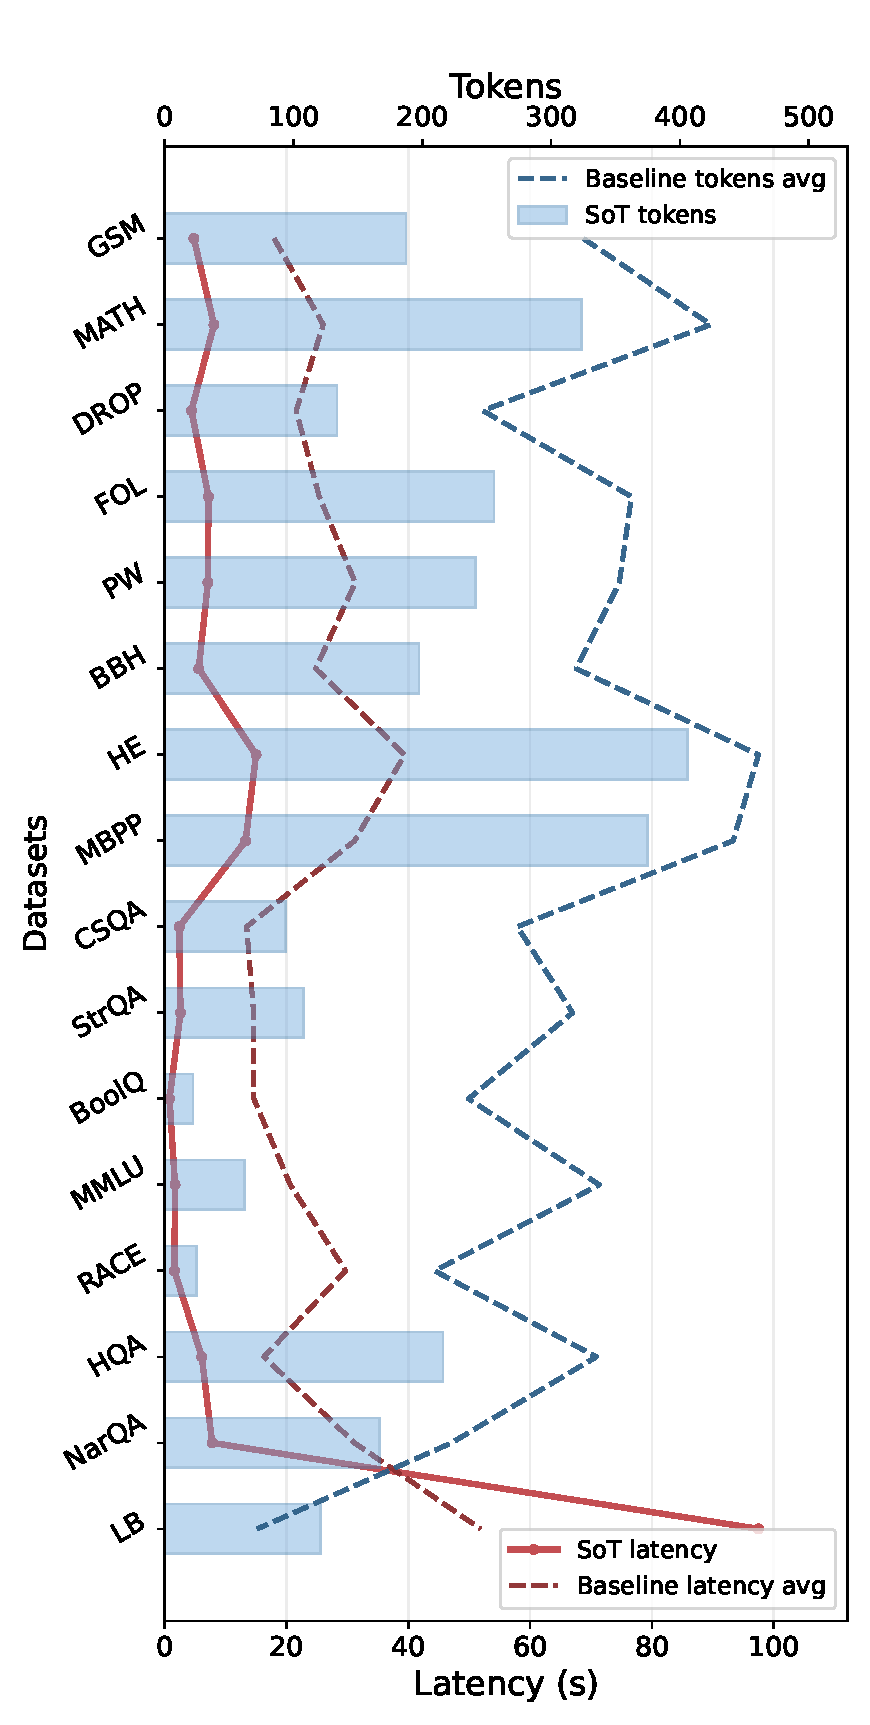
\includegraphics[width=0.94\linewidth]{sot_eff_source.pdf}
\end{minipage}
\end{table}

Averaged over the four reasoning domains, \SoT{} uses 189.8 generated tokens and 9.8 s latency, compared with 532.7 tokens and 33.7 s for sampling/search methods---64.4\% fewer tokens and 70.8\% lower latency. The comparison with memory-oriented methods is equally informative: generic history compression can be cheap but may discard the evidence needed in the current reasoning regime, whereas \SoT{} conditions the retained evidence on the model state.

\begin{figure}[tbp]
\centering
\begin{subfigure}[t]{0.485\textwidth}
\centering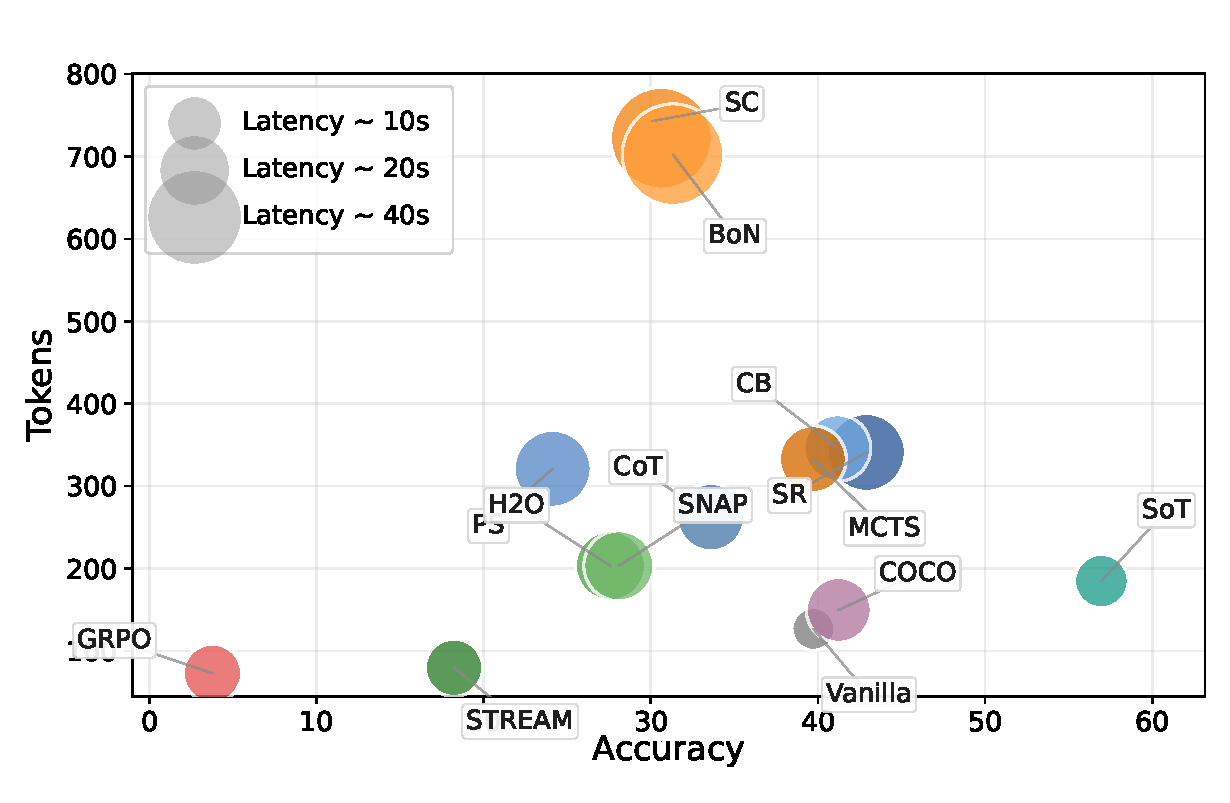
\includegraphics[width=\linewidth]{sot_tradeoff_llama_all.pdf}
\caption{Llama-3.1-8B}
\end{subfigure}\hfill
\begin{subfigure}[t]{0.485\textwidth}
\centering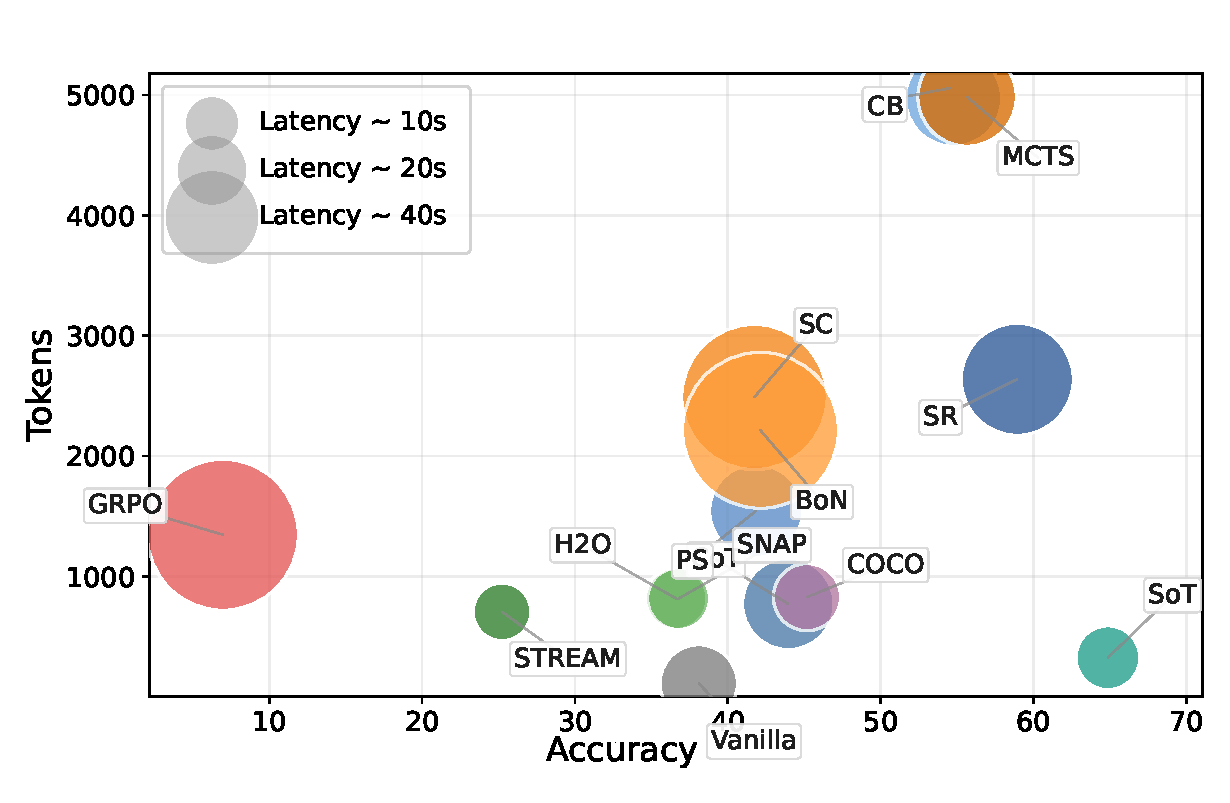
\includegraphics[width=\linewidth]{sot_tradeoff_qwen14b_all.pdf}
\caption{Qwen2.5-14B}
\end{subfigure}

\begin{subfigure}[t]{0.485\textwidth}
\centering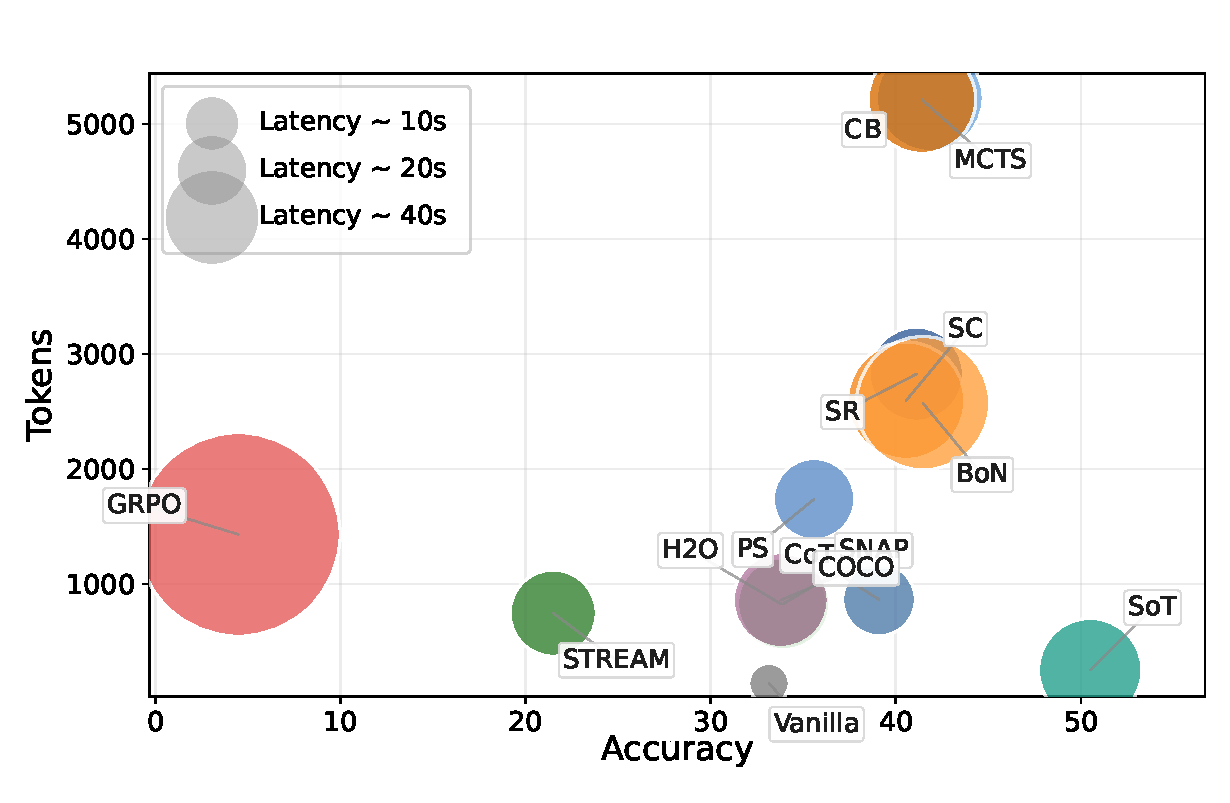
\includegraphics[width=\linewidth]{sot_tradeoff_mixtral_all.pdf}
\caption{Mixtral-8$\times$7B}
\end{subfigure}\hfill
\begin{subfigure}[t]{0.485\textwidth}
\centering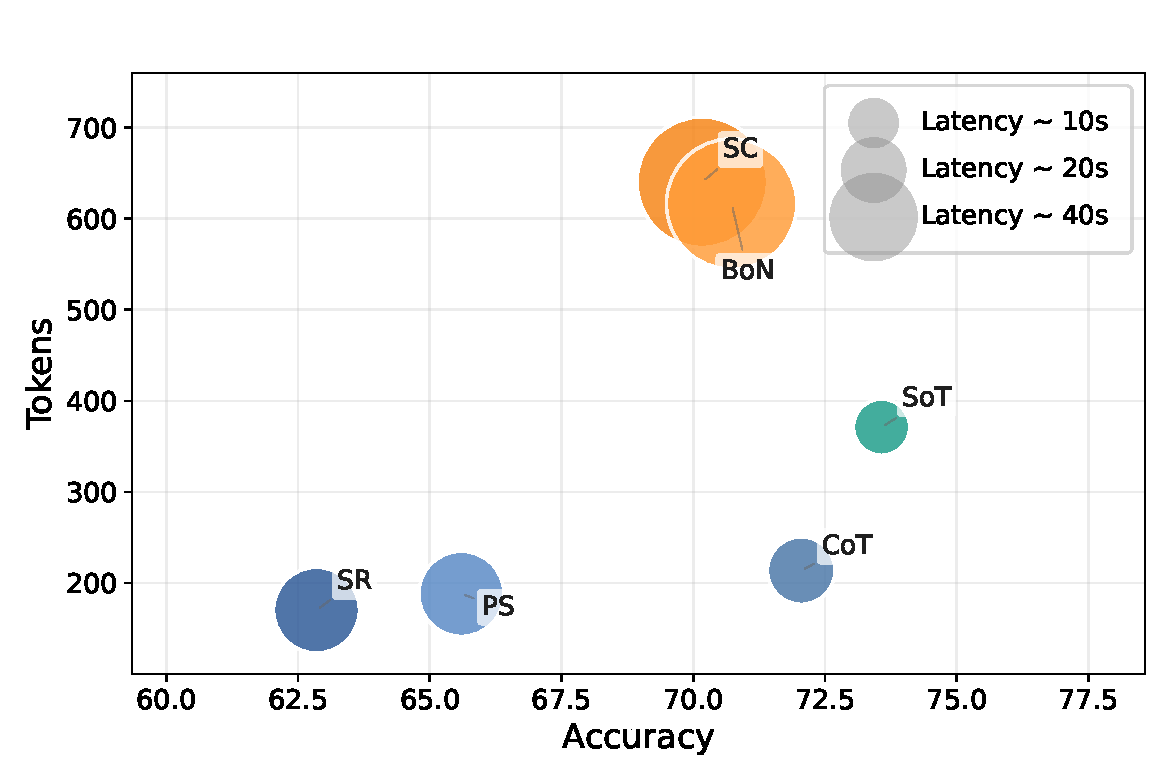
\includegraphics[width=\linewidth]{sot_tradeoff_qwen3vl_all.pdf}
\caption{Qwen3-VL-8B}
\end{subfigure}
\caption{Extended accuracy--efficiency trade-offs across four backbones. Search- and sampling-heavy methods generally move toward higher token/latency regions; \SoT{} remains on or near the high-quality/low-cost frontier across text and multimodal backbones.}
\label{fig:sot-tradeoff-all}
\end{figure}

\textbf{What changes on the frontier?} Search and repeated sampling often buy quality by expanding test-time computation, while generic memory methods reduce context cost without knowing which evidence is useful for the current state. \SoT{} changes the control variable: the same endogenous state determines evidence selection and stopping. The four-backbone view in Figure~\ref{fig:sot-tradeoff-all} shows that this quality--cost shift transfers beyond one model family, while Table~\ref{tab:sot-boundary} tests how much of the gain survives with weaker access to the internal state.

\subsubsection{Exploratory extensions: weaker access assumptions}
The main implementation uses hidden-state access and lightweight learned controllers, but the state-conditioned principle can also be tested under weaker access. \textbf{Training-free SoT} keeps the same state interface but replaces learned evidence/stopping operators with deterministic state-compatibility and stability rules. \textbf{SoT-Embed} replaces privileged hidden states with sentence-embedding trajectory features while preserving the same evidence/stopping interface. Table~\ref{tab:sot-boundary} reports domain averages on two backbones.

\begin{table}[tbp]
\centering\singlespacing\scriptsize
\caption{Limited-access boundary studies of \SoT{} (domain-average accuracy, \%). ``Top-3'' is the mean of the three strongest baselines in the corresponding appendix comparison.}
\label{tab:sot-boundary}
\setlength{\tabcolsep}{3.6pt}\renewcommand{\arraystretch}{1.04}
\begin{tabular}{llrrrr}
\toprule
\textbf{Backbone} & \textbf{Method} & \textbf{Quant.} & \textbf{Sym./Code} & \textbf{General} & \textbf{Long-ctx.}\\
\midrule
\multirow{3}{*}{Qwen2.5-14B} & Top-3 baseline avg. & 63.2 & 60.8 & 57.3 & 17.6\\
& Training-free SoT & 59.1 & 52.0 & 56.5 & \textbf{26.2}\\
& SoT-Embed & 57.9 & 56.0 & 51.3 & 18.1\\
\midrule
\multirow{3}{*}{Mixtral-8$\times$7B} & Top-3 baseline avg. & 40.8 & 43.8 & 65.3 & 22.7\\
& Training-free SoT & 53.2 & \textbf{50.0} & 53.9 & 21.5\\
& SoT-Embed & \textbf{54.1} & 49.8 & 49.0 & \textbf{23.3}\\
\bottomrule
\end{tabular}
\end{table}

These variants are not substitutes for the full controller; they test whether the thesis survives reduced access. The result is intentionally reported as a boundary study: state-conditioned control remains useful in several regimes without learned routing or privileged hidden states, while other domains still benefit from the richer internal signal.

\subsubsection{Ablations: both actions and all state components matter}
The paper removes the evidence organizer, the stop controller, and individual state components. Two failures are especially diagnostic. Without $\mathcal S$, quantitative accuracy drops from 62.8 to 29.6 while token/latency grow markedly; without $\mathcal T$, generated trajectories explode into the thousands of tokens without a consistent accuracy gain. Removing geometry, dynamics, or uncertainty also changes the quality--cost balance. The controller is therefore not equivalent to a learned length threshold or a generic memory selector: it requires a state representation and two coordinated actions.

Table~\ref{tab:sot-ablation} closes the method loop by removing the state features and control actions one at a time.
\begin{table}[tbp]
\centering\singlespacing\scriptsize
\caption{\SoT{} ablation results on Llama-3.1-8B. Each cell reports accuracy / generated tokens / latency (s), aggregated by reasoning domain. The full set of main ablations shows that both control actions and each state component contribute to the quality--cost balance.}
\label{tab:sot-ablation}
\setlength{\tabcolsep}{2.5pt}
\begin{adjustbox}{max width=\textwidth}
\begin{tabular}{lcccc}
\toprule
\textbf{Variant} & \textbf{Quantitative} & \textbf{Symbolic/code} & \textbf{General} & \textbf{Long-context}\\
\midrule
Full \SoT{} & 62.8 / 219.4 / 5.8 & 54.5 / 294.0 / 9.5 & 71.2 / 64.0 / 1.8 & 33.0 / 181.6 / 22.0\\
+ threshold tuning & 62.8 / 219.4 / 5.8 & 54.3 / 294.0 / 9.5 & 71.2 / 64.0 / 1.8 & 31.8 / 229.0 / 22.0\\
\midrule
w/o evidence organizer $\mathcal S$ & 29.6 / 469.5 / 12.9 & 44.5 / 536.2 / 16.5 & 72.4 / 193.9 / 4.9 & 26.9 / 506.5 / 14.1\\
w/o stopping $\mathcal T$ & 60.6 / 1769.6 / 80.7 & 57.1 / 1705.1 / 110.3 & 70.2 / 4148.5 / 99.5 & 31.6 / 2937.4 / 157.3\\
w/o geometry $\delta_t$ & 42.5 / 68.6 / 3.3 & 46.4 / 48.0 / 2.9 & 73.0 / 25.4 / 0.9 & 24.5 / 47.2 / 2.2\\
w/o dynamics $(v_t,c_t)$ & 57.0 / 1039.2 / 29.1 & 46.2 / 846.7 / 25.7 & 71.2 / 1272.3 / 33.7 & 31.6 / 1000.3 / 30.8\\
w/o uncertainty $H_t$ & 54.1 / 244.9 / 6.4 & 52.1 / 281.8 / 8.8 & 73.6 / 61.3 / 1.9 & 32.8 / 555.5 / 16.6\\
w/o sentence-level units & 54.1 / 244.9 / 7.2 & 52.1 / 281.8 / 8.8 & 73.6 / 61.3 / 1.9 & 35.1 / 224.1 / 11.9\\
\bottomrule
\end{tabular}
\end{adjustbox}
\end{table}

\begin{insightbox}
\textbf{What \SoT{} adds to the thesis.} Adaptive computation is not only a parameter-allocation problem. At test time the useful evidence and useful depth also change. \SoT{} moves the control variable from an external reasoning script to an endogenous state, giving the model a closed loop over \emph{evidence} and \emph{continuation}.
\end{insightbox}

\subsection{Logic-Conditioned Internal Pathway Routing with \LoTR{} \texorpdfstring{\projecticon{https://gongzhiren.github.io/LoTR-website/}}{}}
\label{sec:lotr}

\textbf{Problem and idea.} A reasoning paradigm determines the outer procedure---for example, whether the model follows a chain, revises an answer, samples several candidates, or searches a tree. Yet each step is still executed by the same frozen Transformer, even though exploration, consolidation, verification, and resolution can require different internal computation. \LoTR{} treats these recurring logic regimes as a second control layer. It leaves the outer paradigm unchanged, infers the logic state of the current step, and softly routes the next step through a reusable head pathway matched to that state~\citep{gong2026lotr}.

Figure~\ref{fig:lotr} gives the high-level architecture of the plug-in router before its logic-state and pathway components are defined.
\begin{figure}[tbp]
\centering
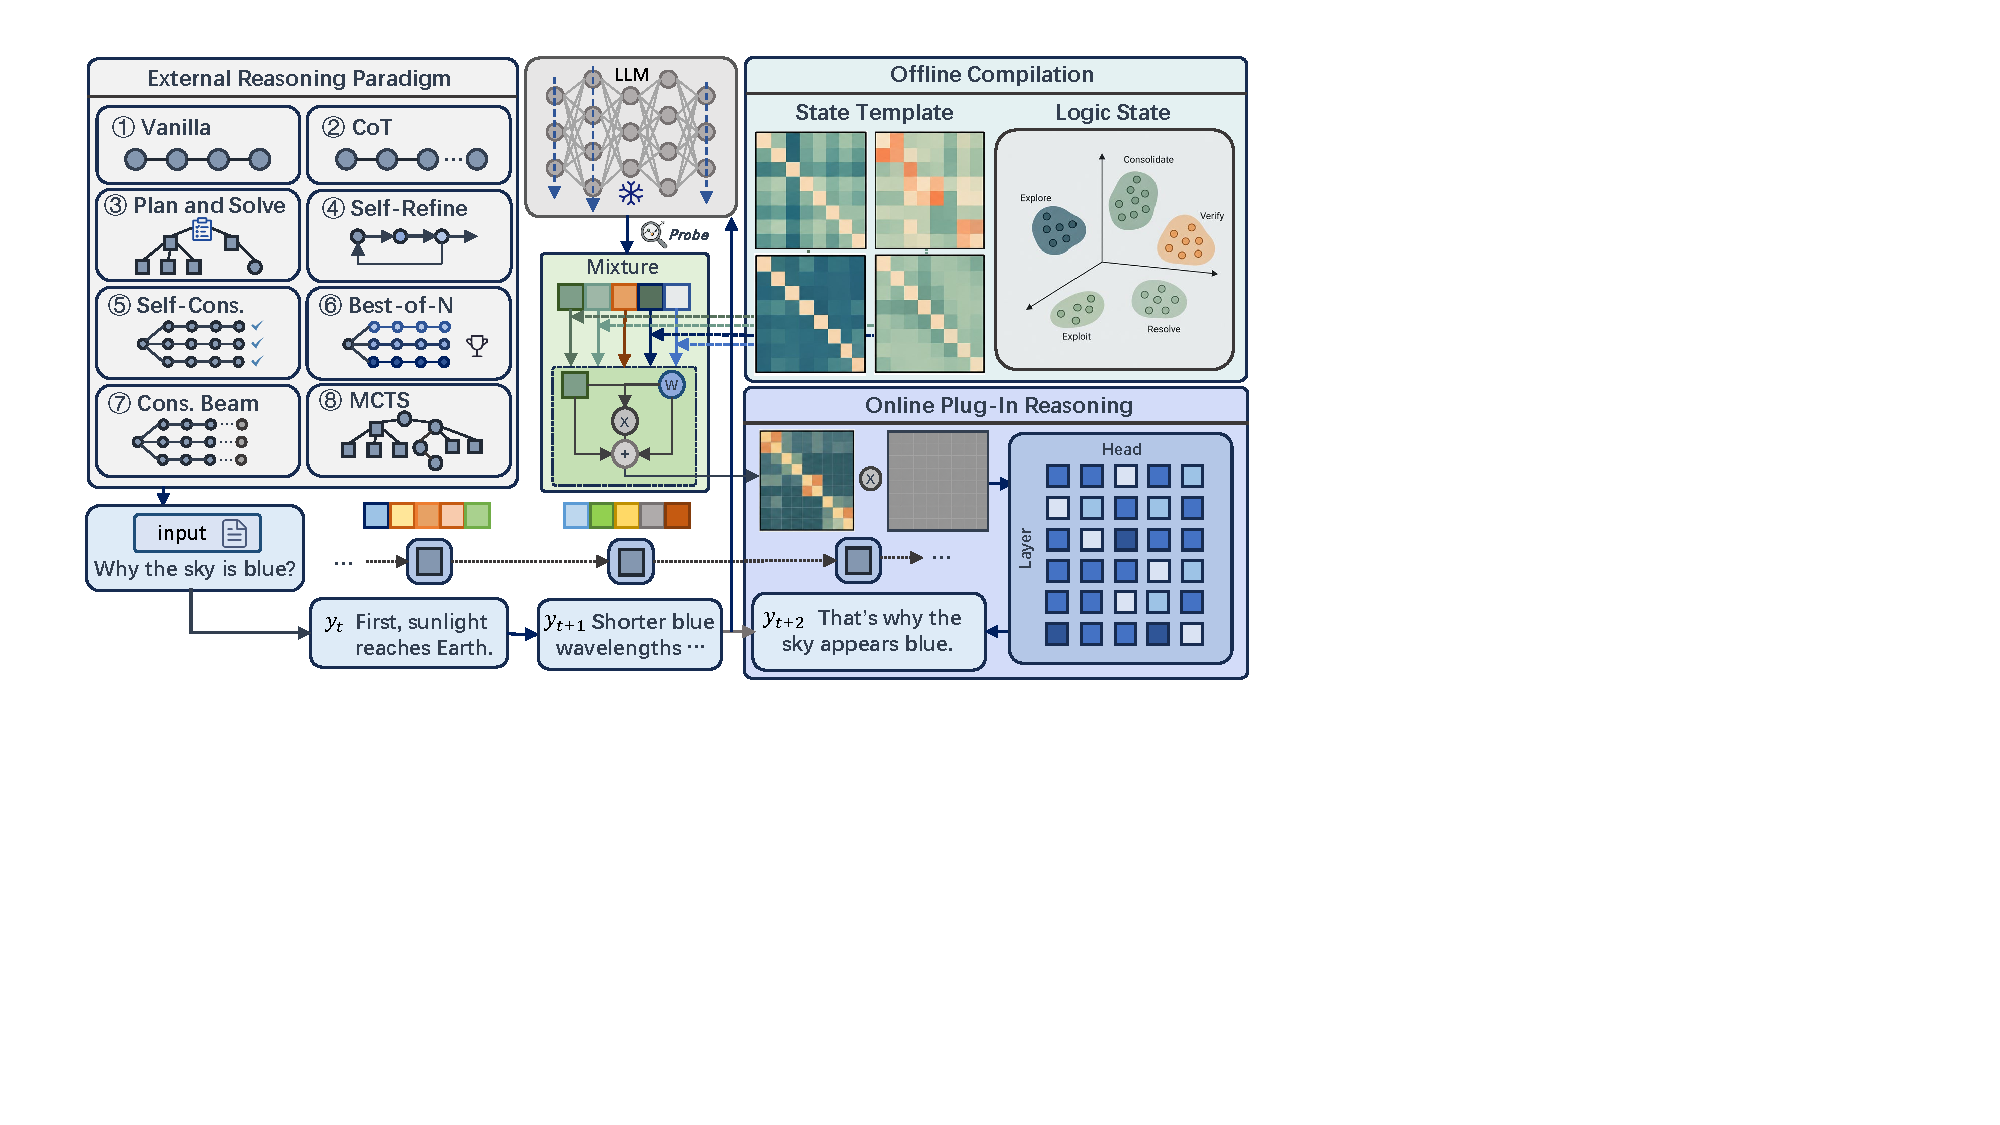
\includegraphics[width=0.91\textwidth]{lotr_intro_main.pdf}
\caption{\LoTR{} pipeline. Multiple external reasoning paradigms are left unchanged; offline logic-state modeling and head-template caching provide an internal control surface that is read and mixed online at sentence boundaries~\citep{gong2026lotr}.}
\label{fig:lotr}
\end{figure}

\subsubsection{Problem formulation: external strategy versus internal pathway}
For frozen Transformer head inventory $\mathcal H$, let
\begin{equation}
\mathcal P_t=\{\gamma_t^{(\ell,h)}\}_{(\ell,h)\in\mathcal H}
\label{eq:lotr-path}
\end{equation}
be the soft head participation pattern used to execute reasoning step $t$. Standard CoT, Self-Refine, Self-Consistency, Best-of-$N$, constrained beam, and MCTS change the \emph{outer} trajectory, but normally leave $\mathcal P_t$ determined by the frozen backbone. \LoTR{} introduces a plug-in controller between the two: infer the recurring logic regime of the current step, then compose the next step's internal pathway from cached state-specific templates.


\subsubsection{Offline logic basis and soft state targets}
Reasoning steps from many paradigms are pooled and represented by sentence-level internal readouts $r_t$. Clustering yields recurring logic centroids $c_1,\ldots,c_K$. Rather than assign a hard label, the target occupancy is softened by distance,
\begin{equation}
\alpha_t^\star(k)=
\exp\!\left(-\frac{\|r_t-c_k\|_2^2}{\tau d_k^2}\right),
\label{eq:lotr-soft}
\end{equation}
where $d_k$ normalizes cluster scale. This matters because a reasoning sentence can simultaneously express, for example, verification and constraint resolution. Layer-wise probes then predict the occupancy from the layer-local readout,
\begin{equation}
\pi_t^{(\ell)}=\sigma\!\left(A^{(\ell)}r_t^{(\ell)}+b^{(\ell)}\right).
\label{eq:lotr-probe}
\end{equation}

The state basis is not only a hidden-space visualization. The analysis shows recurring trajectories across external paradigms and, independently, state-specific head patterns. The two are shown together in Figure~\ref{fig:lotr-structure}.

\begin{figure}[tbp]
\centering
\begin{subfigure}[t]{0.90\textwidth}
\centering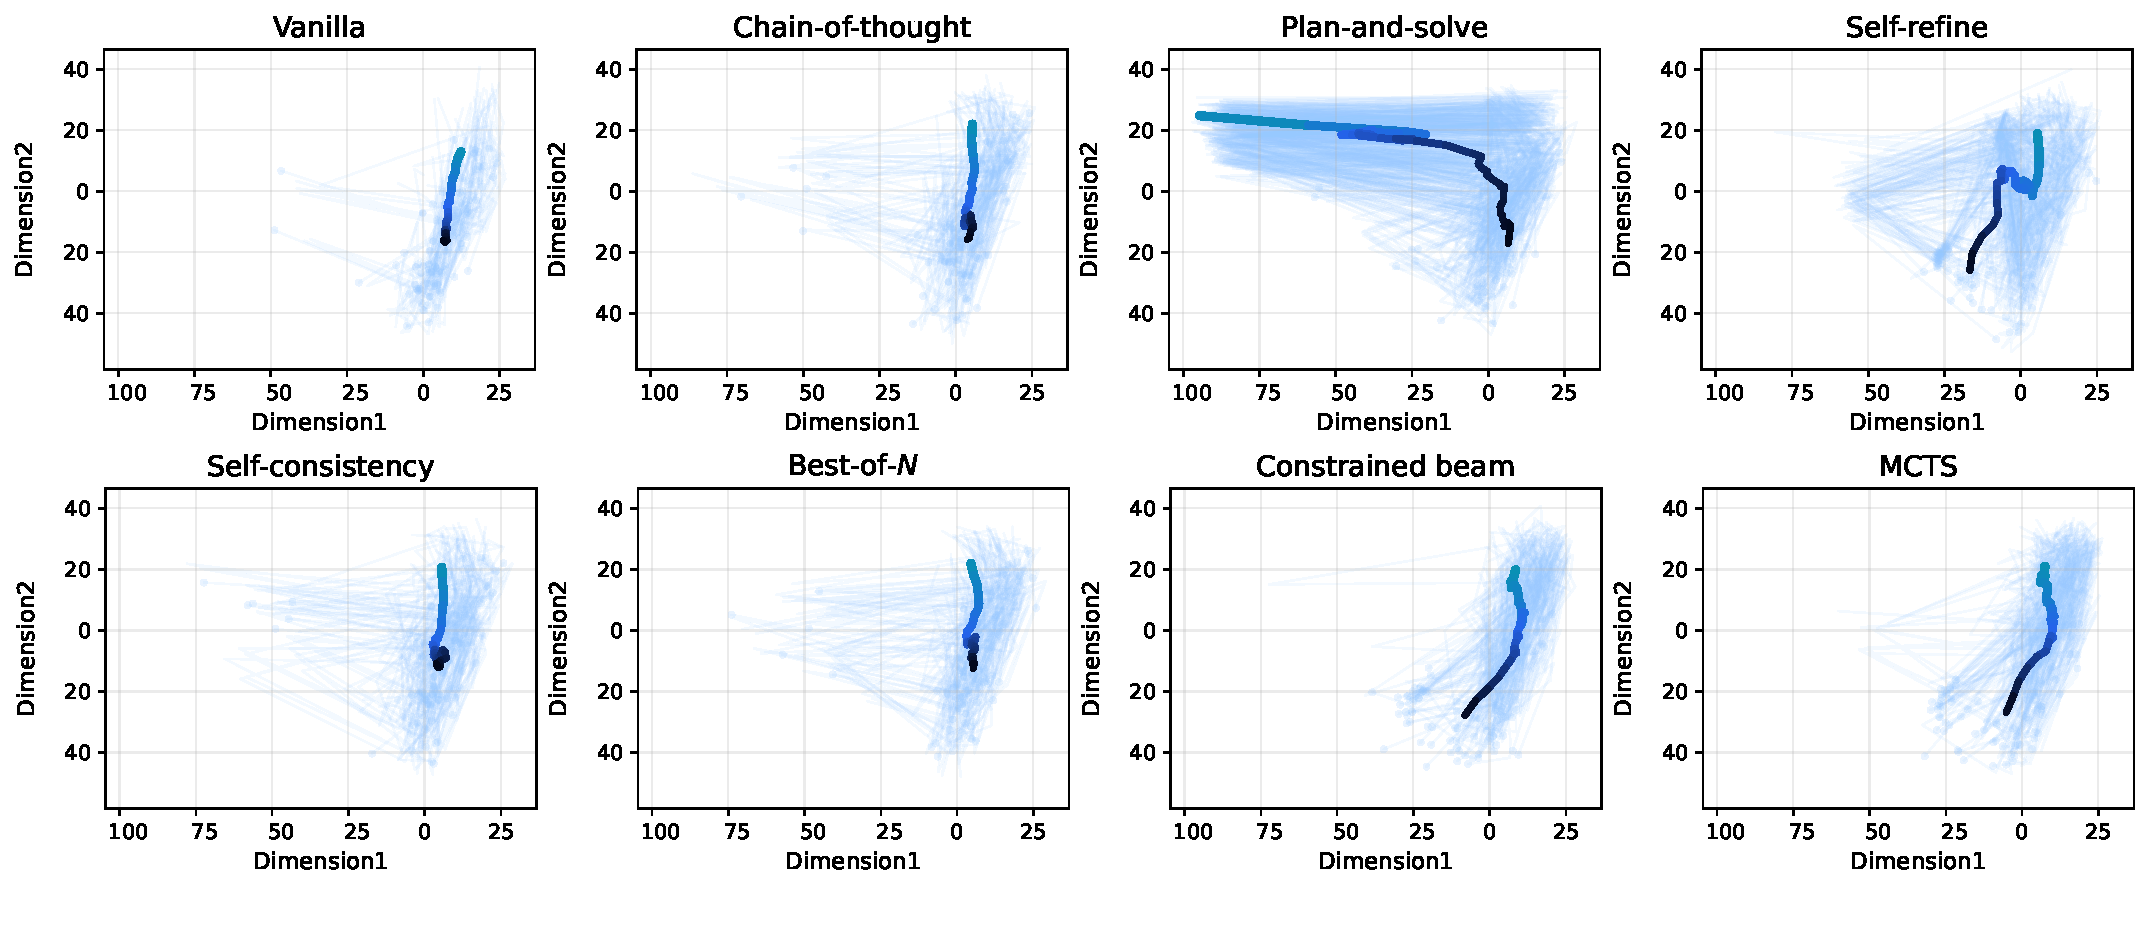
\includegraphics[width=\linewidth]{lotr_logic_trajectories_full.pdf}
\caption{Recurring logic-state trajectories across eight external reasoning paradigms.}
\end{subfigure}

\vspace{2mm}
\begin{subfigure}[t]{0.90\textwidth}
\centering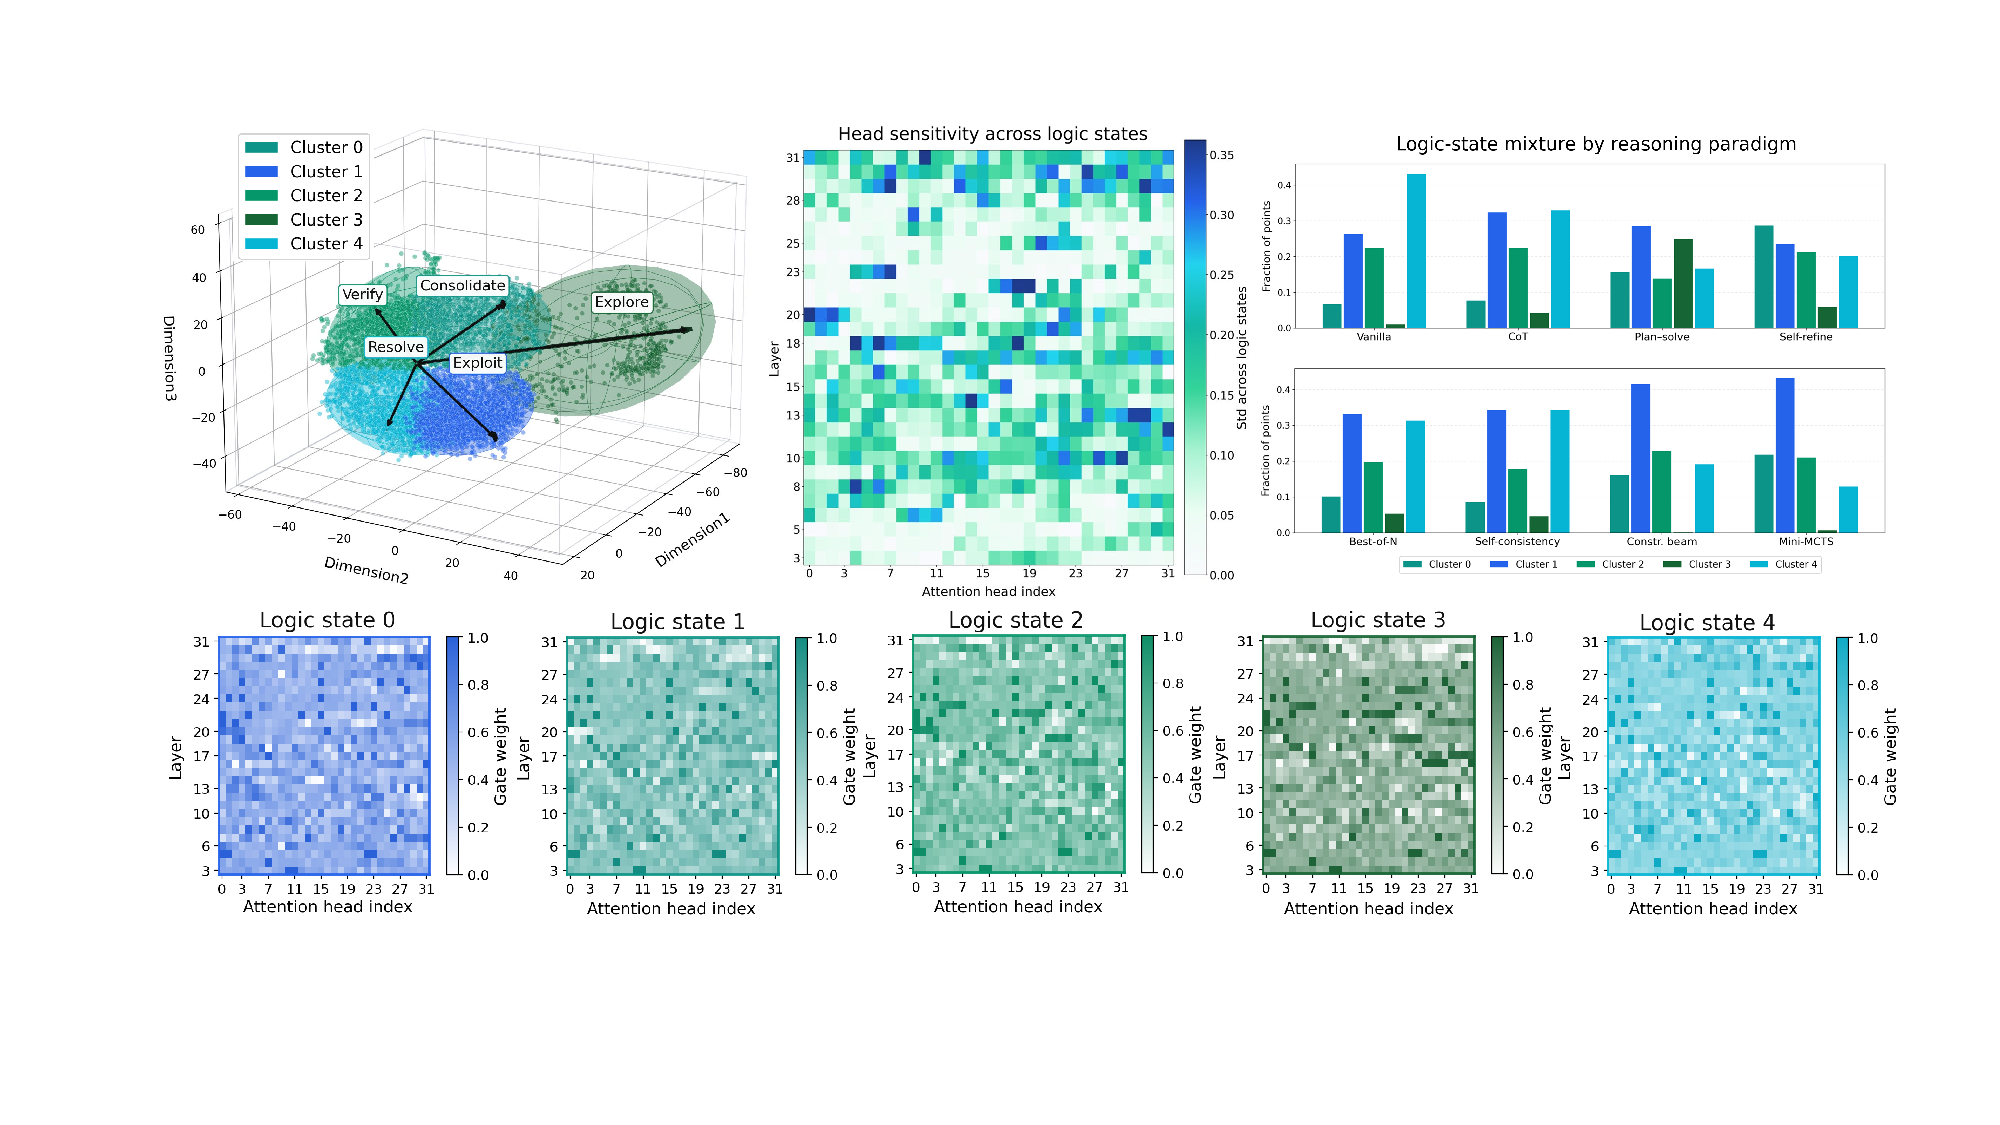
\includegraphics[width=\linewidth]{lotr_pathway_patterns_full.pdf}
\caption{State-specific head pathway patterns compiled from internal information transfer.}
\end{subfigure}
\caption{Two structural observations behind \LoTR{}. Recurring logic regimes appear across different external paradigms, and these regimes are coupled to distinct reusable head-level templates~\citep{gong2026lotr}.}
\label{fig:lotr-structure}
\end{figure}

\subsubsection{Caching logic-conditioned head templates}
For each logic state $k$, a state-specific head score is constructed from the same general kind of representation--parameter coupling used earlier in \SubspacePath{}. If $u_k$ is a direction associated with logic state $k$ and $v_{\ell,h}(t)$ is head $(\ell,h)$'s projected write at reasoning step $t$,
\begin{equation}
J_{\ell,h,k}=\mathbb E_{t:r_t\in C_k}
\frac{(u_k^\top v_{\ell,h}(t))^2}{\|v_{\ell,h}(t)\|_2^2+\epsilon}.
\label{eq:lotr-importance}
\end{equation}
These statistics are converted into reusable templates $T_k^{(\ell,h)}$. The expensive structure is therefore compiled offline; online routing does not search over masks or optimize the backbone.

\subsubsection{Online soft pathway routing}
At each sentence boundary, layer-wise probes read the current logic mixture. The pathway for the next step is a convex-style composition of cached templates:
\begin{equation}
\gamma_{t+1}^{(\ell,h)}=
\operatorname{clip}\!\left(
\sum_{k=1}^{K}\pi_t^{(\ell)}(k)T_k^{(\ell,h)},0,1
\right).
\label{eq:lotr}
\end{equation}
Here $\pi_t^{(\ell)}$ is the layer-local predicted logic-state mixture and $T_k^{(\ell,h)}$ is the cached head template for state $k$. The coefficients are applied directly to the corresponding head outputs. This design is intentionally plug-in: the prompt, sampler, beam, self-refinement loop, or MCTS controller is untouched. Consequently, any consistent improvement can be attributed to a previously unmanaged layer of reasoning---\textbf{internal pathway execution}.

\subsubsection{Evaluation: one internal controller across eight outer paradigms}
The main evaluation is deliberately paired: eight external reasoning paradigms are run both without and with internal steering on eight benchmarks and three backbones. This tests whether an internal router adds value \emph{across} outer algorithms rather than replacing them.

Figure~\ref{fig:lotr-radar} summarizes transfer across paradigms and backbones together with the associated token/latency behavior.
\begin{figure}[tbp]
\centering
\begin{subfigure}[t]{0.52\textwidth}
\centering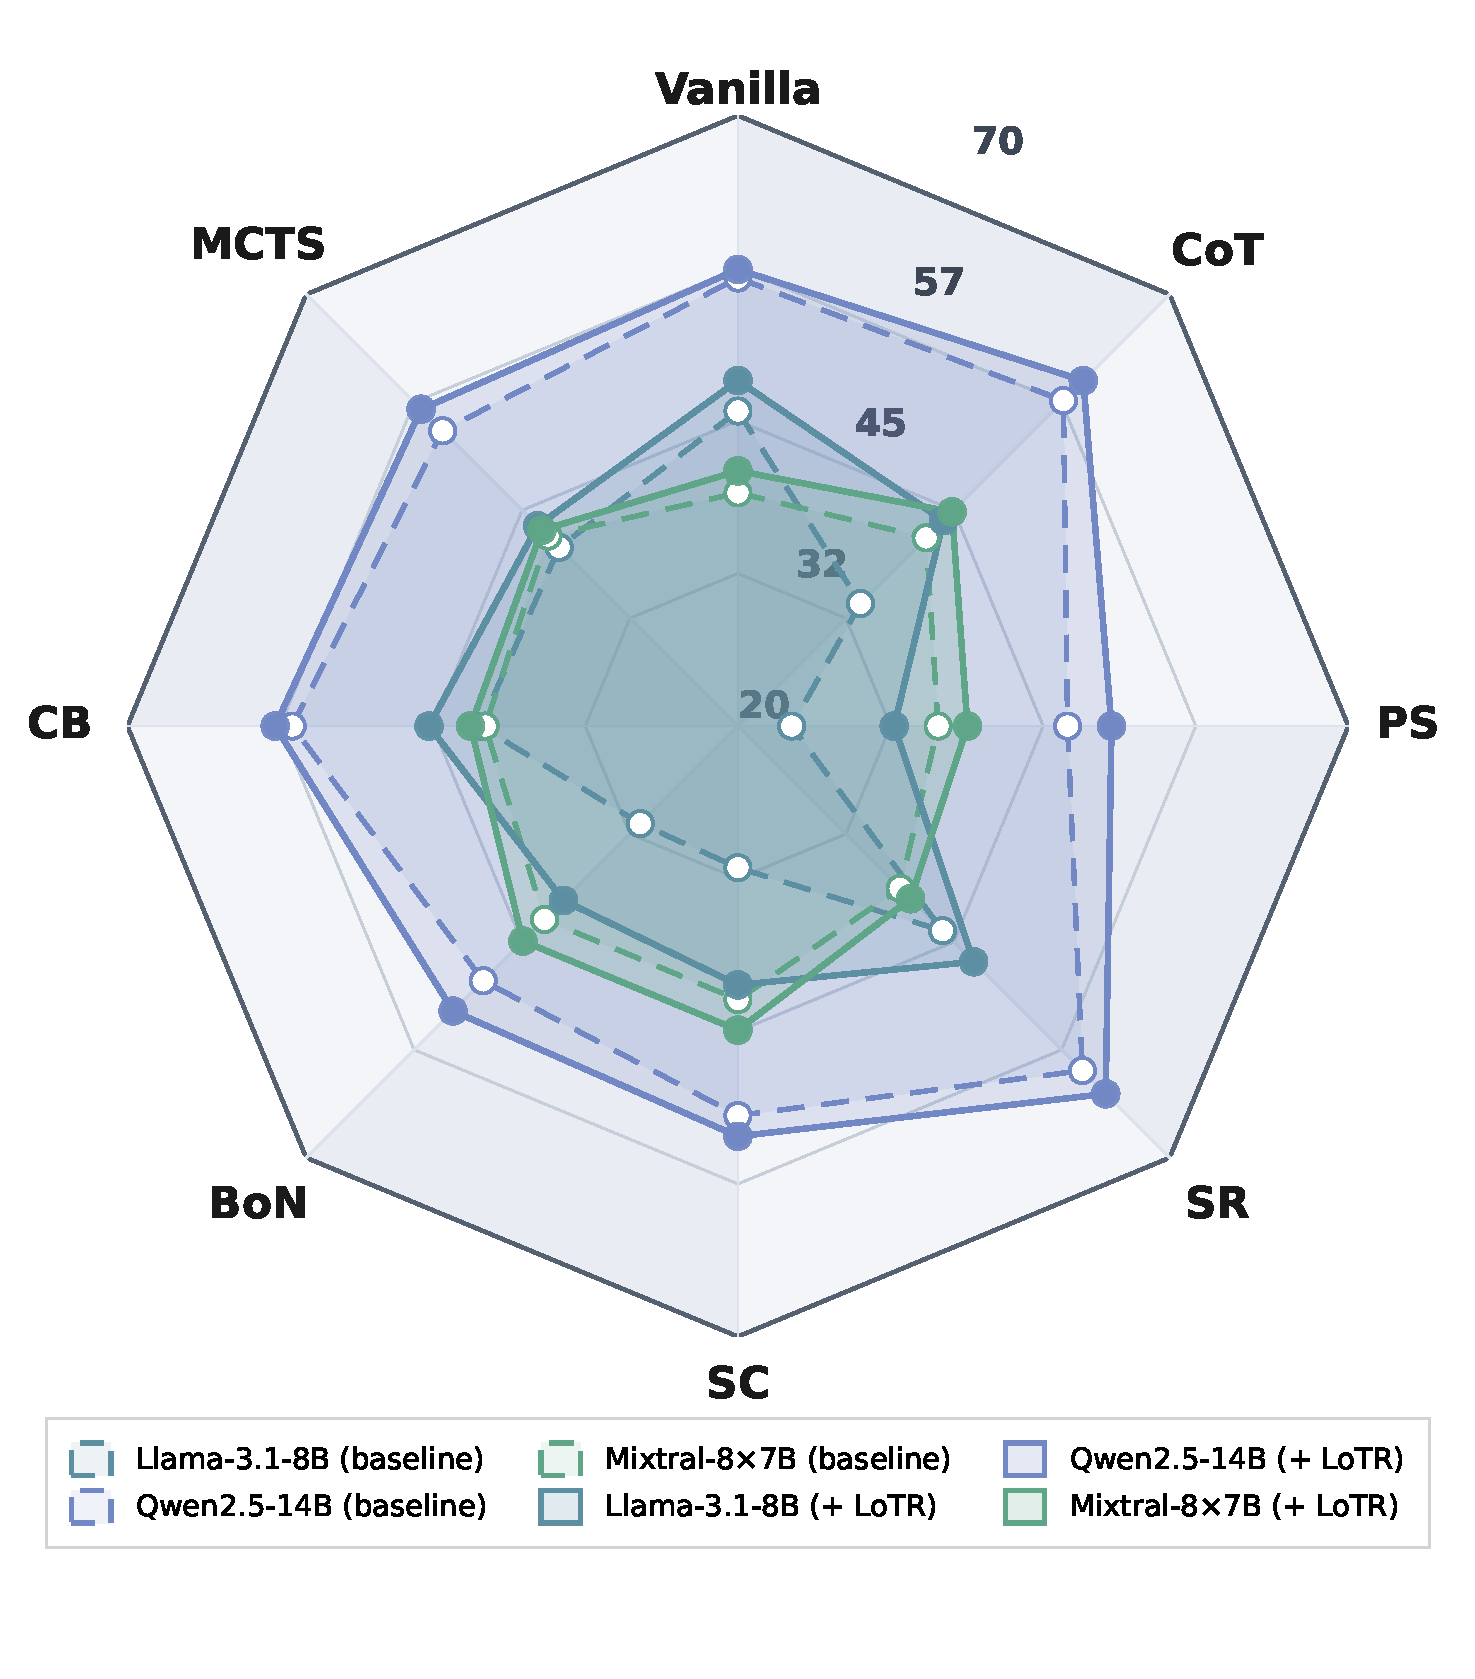
\includegraphics[width=\linewidth]{lotr_intro_radar_three_models.pdf}
\caption{Accuracy change across eight outer reasoning paradigms and three backbones.}
\end{subfigure}\hfill
\begin{subfigure}[t]{0.44\textwidth}
\centering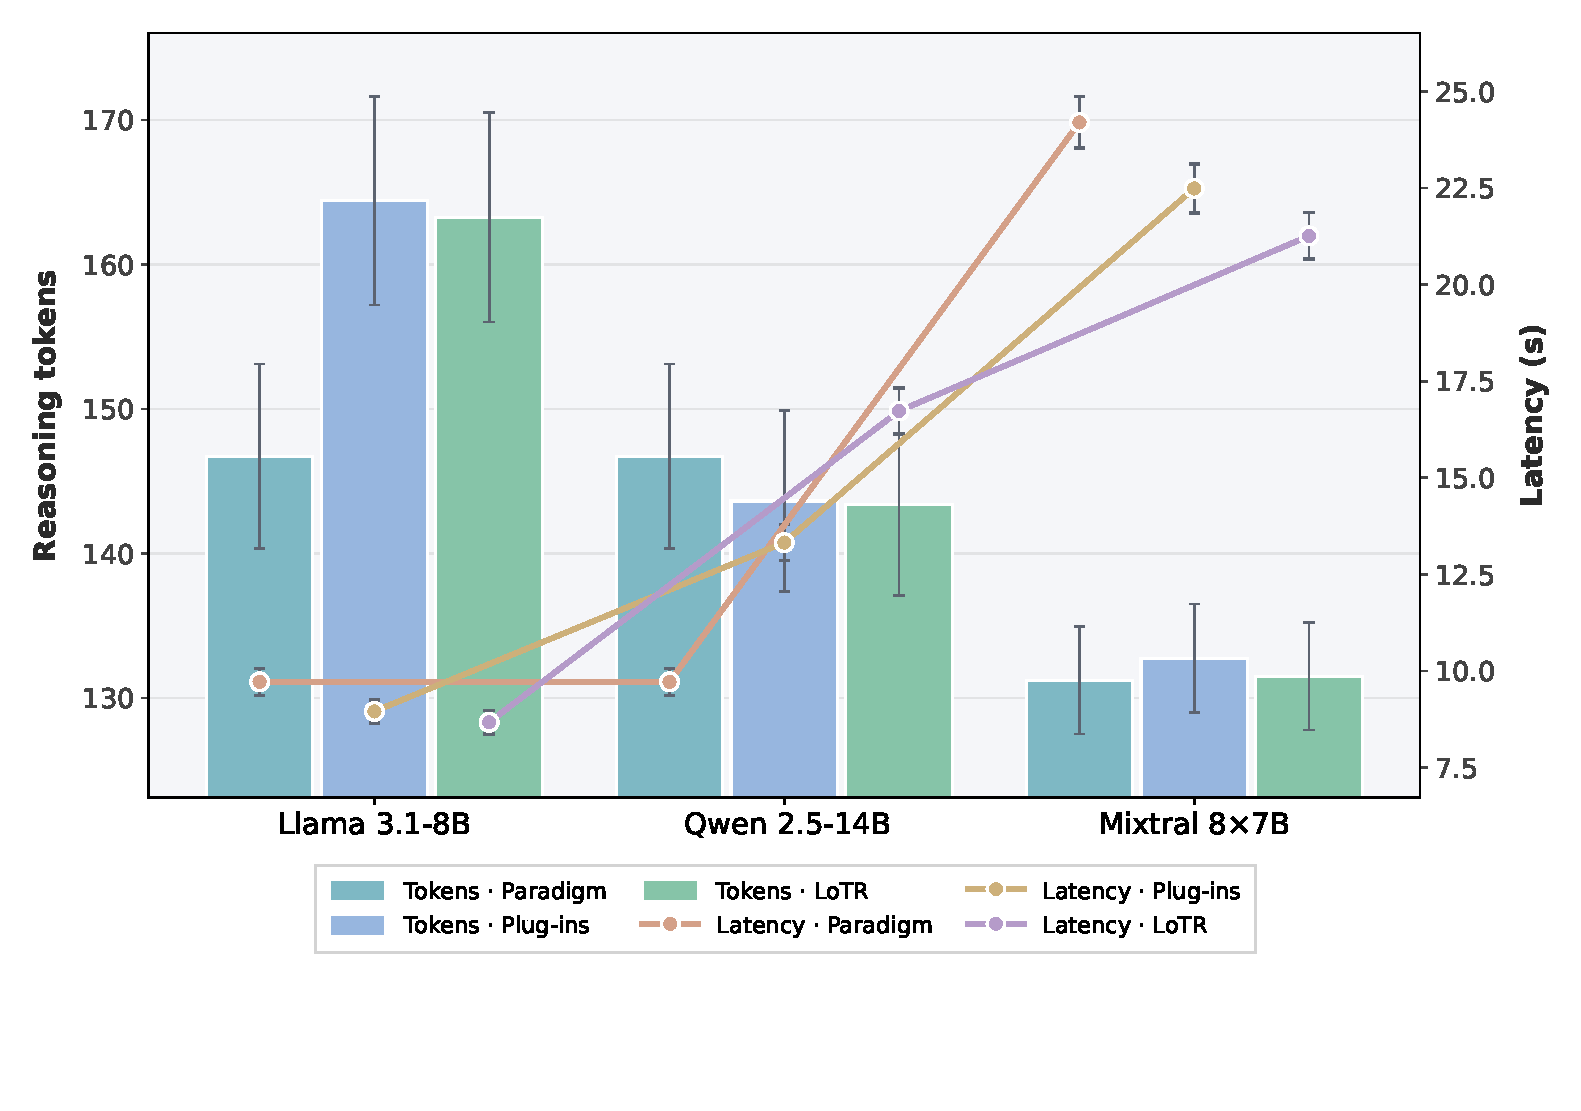
\includegraphics[width=\linewidth]{lotr_intro_efficiency_tokens_latency.pdf}
\caption{Generated-token and latency effects by backbone.}
\end{subfigure}
\caption{Headline transfer and efficiency results of \LoTR{}. Each outer reasoning paradigm is kept fixed; the comparison isolates the contribution of logic-conditioned internal pathway routing.}
\label{fig:lotr-radar}
\end{figure}

\textbf{Cross-paradigm transfer.} The paired design is central to the claim: \LoTR{} is added to the same Vanilla, CoT, Plan-and-Solve, Self-Refine, Self-Consistency, Best-of-$N$, Constrained-Beam, and MCTS procedures rather than replacing them. Improvements across three backbones therefore isolate a control layer that sits \emph{inside} reasoning. The accompanying token/latency panel shows that the gain is not simply purchased by uniformly lengthening every trace.

Table~\ref{tab:lotr-full} gives the paired per-benchmark comparison on Llama-3.1-8B.
\begin{table}[t]
\centering\singlespacing\scriptsize
\caption{Paired Llama-3.1-8B results across eight external reasoning paradigms and eight benchmarks. Each paradigm is evaluated unchanged and with \LoTR{} added as an internal-routing plug-in.}
\label{tab:lotr-full}
\setlength{\tabcolsep}{2.5pt}
\begin{adjustbox}{max width=\textwidth}
\begin{tabular}{llrrrrrrrrr}
\toprule
\textbf{Paradigm} & \textbf{Variant} & \textbf{GSM8K} & \textbf{MATH} & \textbf{BoolQ} & \textbf{HumanEval} & \textbf{MMLU} & \textbf{FOLIO} & \textbf{HotpotQA} & \textbf{NarrativeQA} & \textbf{Avg.}\\
\midrule
\multirow{2}{*}{Vanilla} & Base & 78.9 & 54.1 & 74.7 & 62.0 & 40.9 & 29.1 & 7.1 & 19.8 & 45.8\\
& +\LoTR{} & \textbf{82.0} & \textbf{57.0} & \textbf{82.2} & 62.0 & \textbf{45.4} & \textbf{30.0} & \textbf{7.6} & \textbf{19.9} & \textbf{48.3}\\
\midrule
\multirow{2}{*}{CoT} & Base & 75.1 & 55.4 & 32.8 & 53.0 & 33.2 & 18.0 & 2.0 & 4.2 & 34.2\\
& +\LoTR{} & \textbf{79.6} & \textbf{62.5} & \textbf{39.0} & 53.0 & \textbf{37.2} & \textbf{18.7} & \textbf{29.4} & \textbf{30.9} & \textbf{43.8}\\
\midrule
\multirow{2}{*}{Plan-and-Solve} & Base & 68.5 & 34.0 & 13.5 & 24.0 & 29.7 & 20.9 & 1.7 & 2.8 & 24.4\\
& +\LoTR{} & \textbf{72.2} & \textbf{39.2} & \textbf{20.0} & 24.0 & \textbf{32.8} & \textbf{21.7} & \textbf{21.4} & \textbf{31.0} & \textbf{32.8}\\
\midrule
\multirow{2}{*}{Self-Refine} & Base & 69.6 & 38.4 & 68.2 & 50.0 & 56.4 & 29.8 & 15.8 & 21.6 & 43.7\\
& +\LoTR{} & \textbf{75.8} & \textbf{46.0} & \textbf{71.5} & 50.0 & \textbf{58.4} & \textbf{30.5} & \textbf{17.3} & \textbf{29.0} & \textbf{47.3}\\
\midrule
\multirow{2}{*}{Self-Consistency} & Base & 79.7 & 47.7 & 40.1 & 35.0 & 24.6 & 19.4 & 1.9 & 4.1 & 31.6\\
& +\LoTR{} & \textbf{84.4} & \textbf{55.2} & \textbf{41.8} & \textbf{41.0} & \textbf{32.0} & 18.7 & \textbf{26.0} & \textbf{30.7} & \textbf{41.2}\\
\midrule
\multirow{2}{*}{Best-of-$N$} & Base & 79.6 & 46.8 & 39.3 & 35.0 & 24.9 & 19.1 & 1.9 & 4.0 & 31.3\\
& +\LoTR{} & \textbf{85.2} & \textbf{53.5} & 39.2 & 34.0 & \textbf{32.2} & \textbf{20.2} & \textbf{26.7} & \textbf{31.0} & \textbf{40.2}\\
\midrule
\multirow{2}{*}{Constr. Beam} & Base & 43.1 & 26.4 & 80.4 & 52.4 & 45.4 & 38.3 & 15.7 & 27.2 & 41.1\\
& +\LoTR{} & \textbf{46.8} & \textbf{37.2} & \textbf{84.8} & \textbf{55.0} & \textbf{53.0} & \textbf{40.9} & 14.9 & \textbf{29.7} & \textbf{45.3}\\
\midrule
\multirow{2}{*}{MCTS} & Base & 51.5 & 28.0 & 75.0 & 54.0 & 42.6 & 34.1 & 13.2 & 26.9 & 40.7\\
& +\LoTR{} & \textbf{52.6} & \textbf{29.0} & \textbf{82.2} & \textbf{58.0} & \textbf{46.8} & \textbf{34.5} & \textbf{13.6} & \textbf{28.6} & \textbf{43.2}\\
\bottomrule
\end{tabular}
\end{adjustbox}
\end{table}

The main study evaluates eight reasoning paradigms on eight benchmarks and three backbones, comparing \LoTR{} with four representative internal-steering plug-ins. The key evaluation design is paired: every outer paradigm is run both unsteered and with each plug-in, so the question is not whether a new reasoning algorithm beats old ones but whether a common internal router can improve many of them.

Table~\ref{tab:lotr-main} then compares \LoTR{} with representative internal-steering plug-ins while holding the outer paradigm fixed.
\begin{table}[tbp]
\centering\singlespacing\scriptsize
\caption{Paradigm-average comparison with four representative internal-steering plug-ins on Llama-3.1-8B. The outer reasoning strategy is fixed row-by-row.}
\label{tab:lotr-main}
\setlength{\tabcolsep}{4.0pt}
\begin{tabular}{lrrrrrr}
\toprule
\textbf{Outer paradigm} & \textbf{Base} & \textbf{ITI} & \textbf{ActAdd} & \textbf{STIR} & \textbf{RISER} & \textbf{\LoTR{}}\\
\midrule
Vanilla & 45.8 & 47.6 & 45.6 & 45.0 & 46.5 & \textbf{48.3}\\
Chain-of-Thought & 34.2 & 43.4 & 42.8 & 42.5 & 41.3 & \textbf{43.8}\\
Plan-and-Solve & 24.4 & 27.7 & 29.5 & 30.5 & 30.3 & \textbf{32.8}\\
Self-Refine & 43.7 & 47.2 & 46.8 & 45.7 & 45.6 & \textbf{47.3}\\
Self-Consistency & 31.6 & 39.2 & 39.7 & 37.1 & 38.1 & \textbf{41.2}\\
Best-of-$N$ & 31.3 & 38.3 & 39.8 & 38.1 & 39.4 & \textbf{40.2}\\
Constrained Beam & 41.1 & 42.5 & 40.7 & 43.3 & 43.1 & \textbf{45.3}\\
MCTS & 40.7 & 42.2 & \textbf{43.4} & 39.5 & 40.9 & 43.2\\
\bottomrule
\end{tabular}
\end{table}

Across 3 backbones $\times$ 8 benchmarks, the paper reports a 7.93\% relative average accuracy gain. Cross-backbone improvements averaged over the paradigm/benchmark grid are +16.67\% on Llama-3.1-8B, +4.25\% on Qwen2.5-14B, and +4.94\% on Mixtral-8$\times$7B. The fact that the same internal interface improves very different wrappers is the main generalization result: logic-state routing is complementary to the external algorithm.



\subsubsection{Efficiency and ablation evidence}
Table~\ref{tab:lotr-efficiency-full} reports the full accuracy/token/latency comparison across the eight outer paradigms.
\begin{table}[tbp]
\centering
\caption{Efficiency of \LoTR{} on Llama-3.1-8B across eight external reasoning paradigms. Tok. is the benchmark-averaged number of generated reasoning tokens and Lat. is end-to-end latency in seconds.}
\label{tab:lotr-efficiency-full}
\vspace{-2mm}
\footnotesize
\setlength{\tabcolsep}{3.2pt}
\renewcommand{\arraystretch}{0.92}

\resizebox{\textwidth}{!}{
    % --- (Vanilla & CoT) ---
    \begin{tabular}{lcc}
    \toprule
    \textbf{Method} & \textbf{Tok.} $\downarrow$ & \textbf{Lat.} $\downarrow$ \\
    \midrule
    Vanilla & 128.6 & 2.87 \\
    + ITI & 112.0 & 2.24 \\
    + ActAdd & 110.1 & 2.62 \\
    + STIR & \underline{109.4} & 2.19 \\
    + RISER & \underline{109.4} & 2.19 \\
    + \textbf{\LoTR{}} & \cellcolor{cyan!10}{\textbf{\underline{109.4}}} & \cellcolor{cyan!10}{\textbf{\underline{2.17}}} \\
    \midrule
    CoT & \underline{258.0} & \underline{5.79} \\
    + ITI & 288.9 & 6.22 \\
    + ActAdd & 286.3 & 6.15 \\
    + STIR & 286.7 & 6.12 \\
    + RISER & 286.7 & 7.23 \\
    + \textbf{\LoTR{}} & \cellcolor{cyan!10}{\textbf{286.7}} & \cellcolor{cyan!10}{\textbf{6.12}} \\
    \bottomrule
    \end{tabular}%
    \hspace{3mm}
    % --- (PS & SR) ---
    \begin{tabular}{lcc}
    \toprule
    \textbf{Method} & \textbf{Tok.} $\downarrow$ & \textbf{Lat.} $\downarrow$ \\
    \midrule
    PS & \underline{196.0} & \underline{5.69} \\
    + ITI & 274.8 & 7.57 \\
    + ActAdd & 272.0 & 7.47 \\
    + STIR & 270.7 & 7.37 \\
    + RISER & 270.7 & 7.63 \\
    + \textbf{\LoTR{}} & \cellcolor{cyan!10}{\textbf{270.7}} & \cellcolor{cyan!10}{\textbf{7.36}} \\
    \midrule
    SR & 50.8 & 8.96 \\
    + ITI & 48.8 & 7.88 \\
    + ActAdd & \underline{45.8} & 7.77 \\
    + STIR & 46.0 & 7.75 \\
    + RISER & 46.0 & 7.78 \\
    + \textbf{\LoTR{}} & \cellcolor{cyan!10}{\textbf{46.0}} & \cellcolor{cyan!10}{\textbf{\underline{7.72}}} \\
    \bottomrule
    \end{tabular}%
    \hspace{3mm}
    % --- (SC & BoN) ---
    \begin{tabular}{lcc}
    \toprule
    \textbf{Method} & \textbf{Tok.} $\downarrow$ & \textbf{Lat.} $\downarrow$ \\
    \midrule
    SC & \underline{242.1} & 18.95 \\
    + ITI & 257.9 & 16.03 \\
    + ActAdd & 255.1 & 15.87 \\
    + STIR & 256.0 & \underline{15.86} \\
    + RISER & 255.8 & 15.90 \\
    + \textbf{\LoTR{}} & \cellcolor{cyan!10}{\textbf{256.4}} & \cellcolor{cyan!10}{\textbf{\underline{15.86}}} \\
    \midrule
    BoN & \underline{242.2} & 16.73 \\
    + ITI & 258.8 & 16.14 \\
    + ActAdd & 256.9 & 15.91 \\
    + STIR & 255.0 & 15.78 \\
    + RISER & 255.1 & 15.93 \\
    + \textbf{\LoTR{}} & \cellcolor{cyan!10}{\textbf{255.6}} & \cellcolor{cyan!10}{\textbf{\underline{15.68}}} \\
    \bottomrule
    \end{tabular}%
    \hspace{3mm}
    % --- (CB & MCTS) ---
    \begin{tabular}{lcc}
    \toprule
    \textbf{Method} & \textbf{Tok.} $\downarrow$ & \textbf{Lat.} $\downarrow$ \\
    \midrule
    CB & \underline{22.0} & 9.15 \\
    + ITI & 44.4 & 7.47 \\
    + ActAdd & 42.1 & 7.46 \\
    + STIR & 40.3 & 7.66 \\
    + RISER & 40.0 & 10.12 \\
    + \textbf{\LoTR{}} & \cellcolor{cyan!10}{\textbf{40.3}} & \cellcolor{cyan!10}{\textbf{\underline{7.32}}} \\
    \midrule
    MCTS & \underline{34.1} & 9.63 \\
    + ITI & 49.9 & 7.43 \\
    + ActAdd & 44.5 & 7.29 \\
    + STIR & 42.7 & 7.24 \\
    + RISER & 42.4 & 8.32 \\
    + \textbf{\LoTR{}} & \cellcolor{cyan!10}{\textbf{41.1}} & \cellcolor{cyan!10}{\textbf{\underline{7.17}}} \\
    \bottomrule
    \end{tabular}
}
\vspace{-2mm}
\end{table}


Routing need not imply a uniformly longer trace. On the Llama backbone, the reported macro-average is approximately 42.8\% accuracy at 163.3 generated tokens and 8.68 s, compared with about 36.6\% / 146.7 tokens / 9.72 s for the unsteered outer paradigms and about 40--41\% / 163--167 tokens / 8.75--9.39 s for strong plug-ins. Some paradigms generate slightly more tokens after routing, but wall-clock latency falls on average because pathway alignment changes the execution dynamics rather than simply extending every chain.

The resulting quality--efficiency frontier is shown in Figure~\ref{fig:lotr-eff}.
\begin{figure}[tbp]
\centering
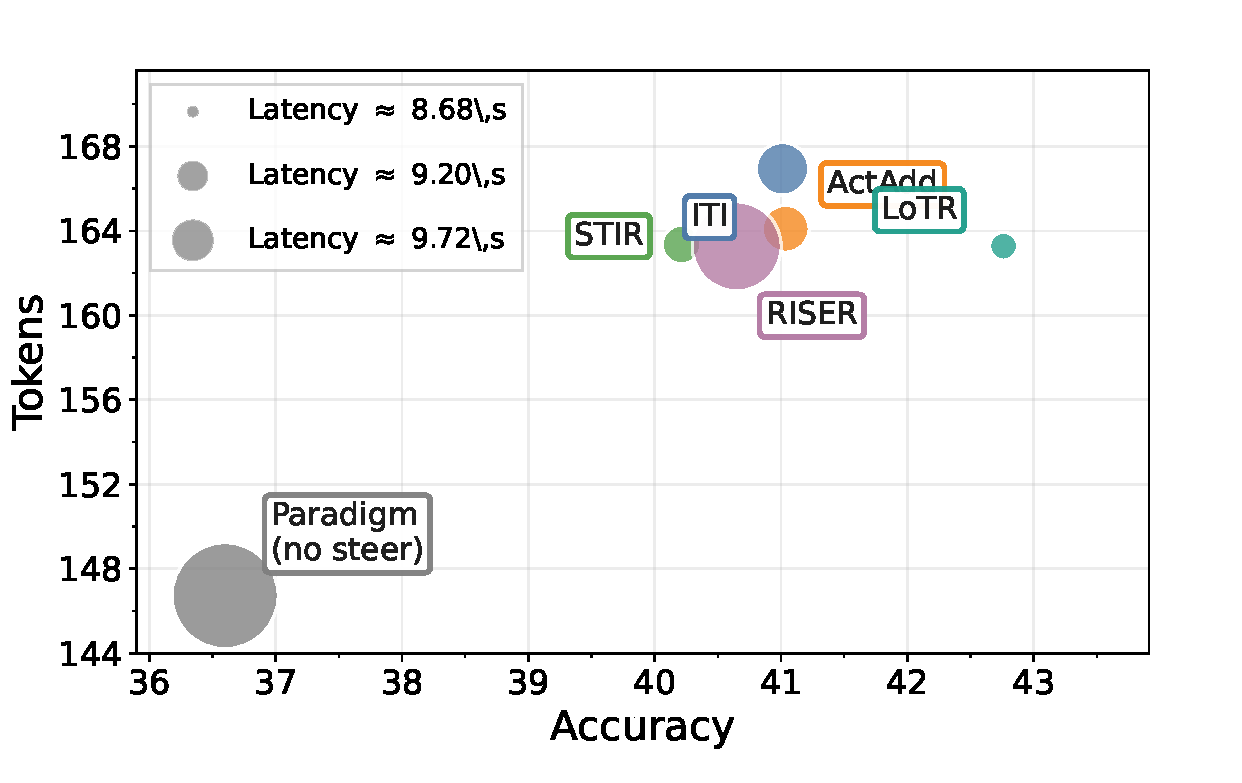
\includegraphics[width=0.70\textwidth]{lotr_tradeoff_full2.pdf}
\caption{Llama-3.1-8B accuracy--efficiency frontier for \LoTR{} and comparison methods~\citep{gong2026lotr}.}
\label{fig:lotr-eff}
\end{figure}

The ablation study removes precisely the structural choices implied by the method. Collapsing to $K=1$, replacing soft targets with hard targets, sharing one probe across layers, using one global template, routing only at trajectory level, or removing state conditioning all weaken the quality--cost balance. The representative Llama-3.1-8B ablations below isolate these design choices.

Table~\ref{tab:lotr-ablation} removes the specific structural choices implied by the method.
\begin{table}[tbp]
\centering\singlespacing\footnotesize
\caption{\LoTR{} ablations. Accuracy/token pairs are shown on three representative benchmarks.}
\label{tab:lotr-ablation}
\setlength{\tabcolsep}{4pt}
\begin{tabular}{lccc}
\toprule
\textbf{Variant} & \textbf{BoolQ} & \textbf{MMLU} & \textbf{HotpotQA}\\
\midrule
Full \LoTR{} & \textbf{60.5}/93.3 & \textbf{43.2}/139.4 & 21.0/137.5\\
Collapsed states ($K=1$) & 60.1/93.6 & 42.8/139.3 & 21.0/139.1\\
Hard targets & 59.5/94.6 & 42.1/140.4 & 19.8/135.5\\
Shared probe & 60.4/92.3 & 42.9/140.5 & 21.0/136.0\\
One global template & 58.8/92.6 & 41.8/138.9 & 21.3/138.1\\
No state conditioning & 58.8/93.0 & 43.1/140.0 & \textbf{21.4}/138.3\\
\bottomrule
\end{tabular}
\end{table}

Figure~\ref{fig:lotr-case} closes the section with one trajectory-level case study of state occupancy and pathway recomposition.
\begin{figure}[tbp]
\centering
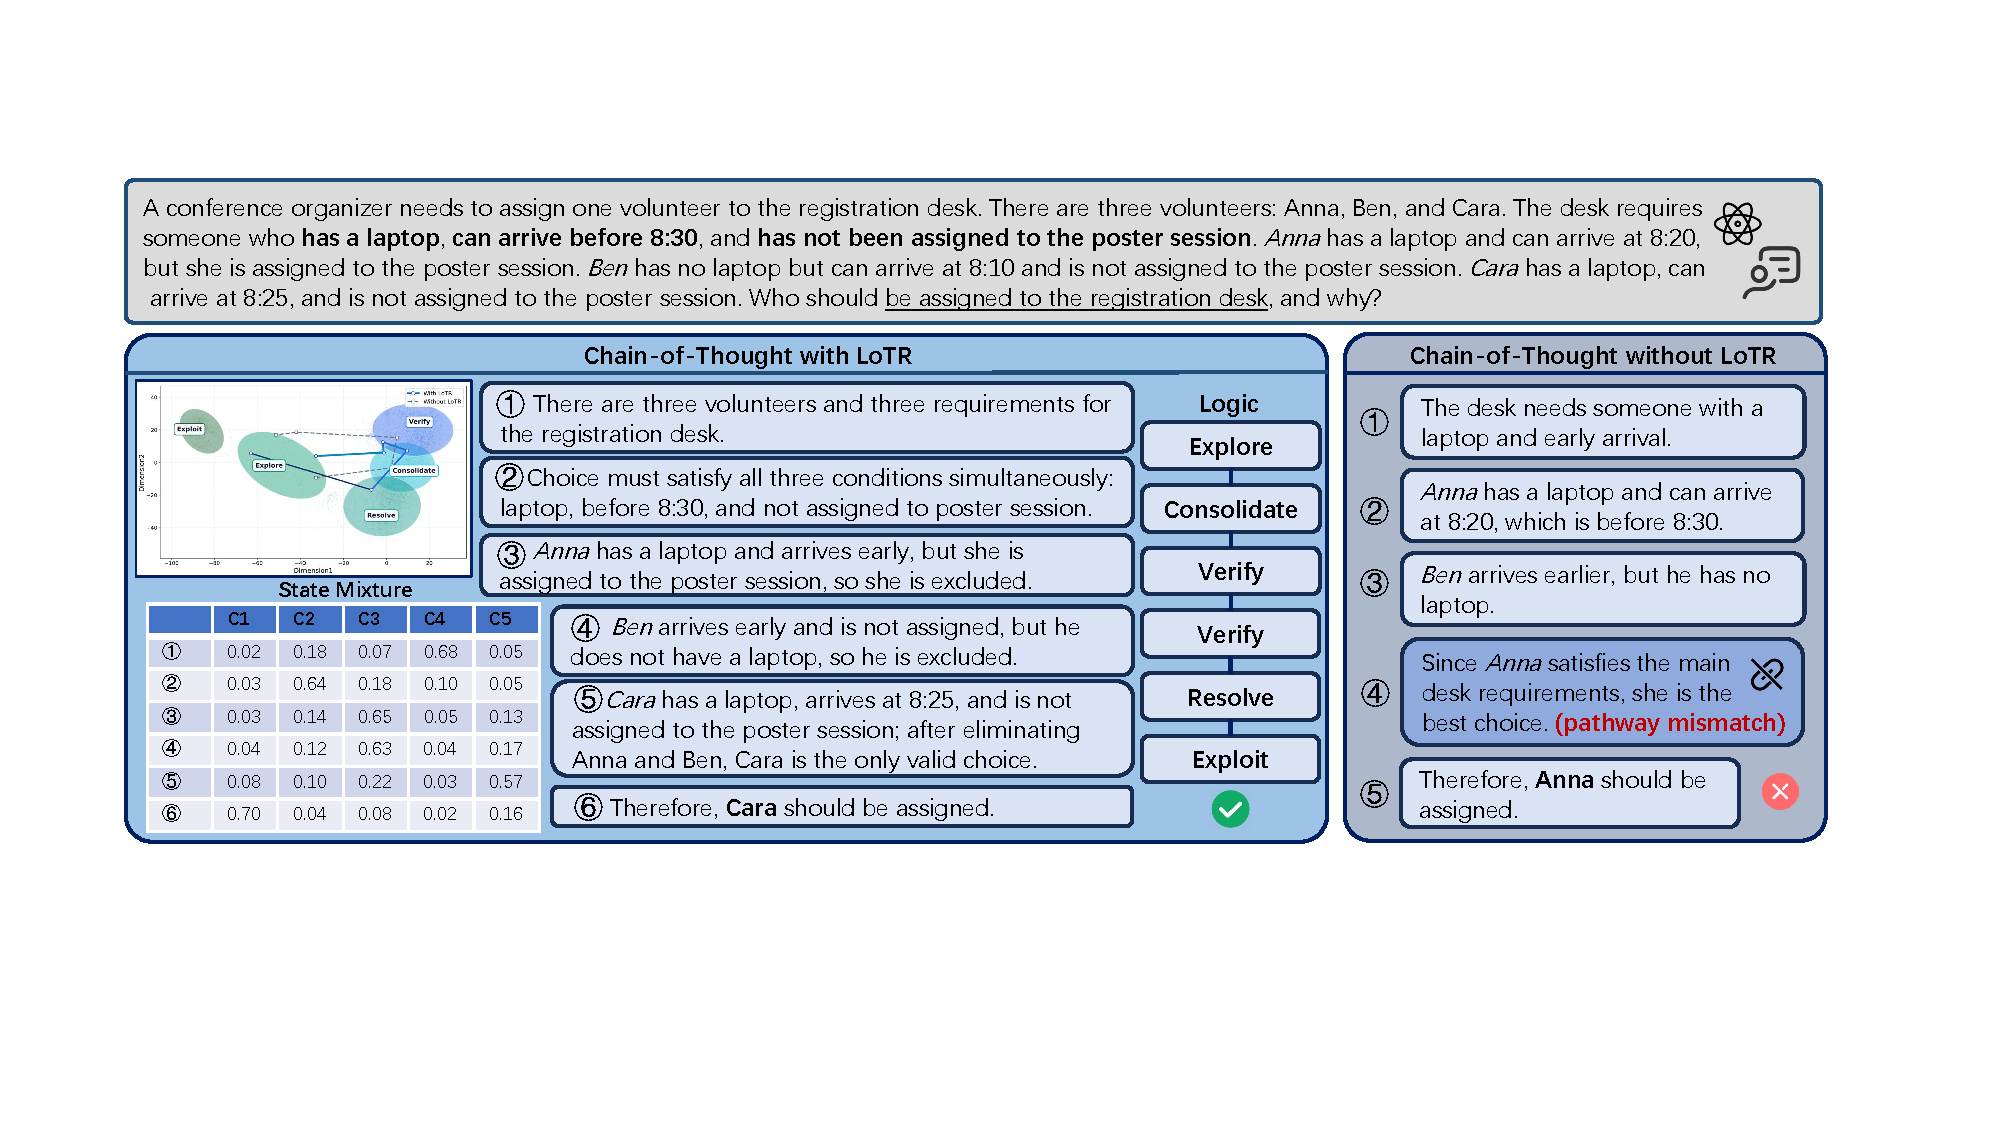
\includegraphics[width=0.88\textwidth]{lotr_case_full.pdf}
\caption{\LoTR{} case study. The example illustrates how inferred logic occupancy changes across a reasoning trajectory and how the internal head pathway is correspondingly recomposed~\citep{gong2026lotr}.}
\label{fig:lotr-case}
\end{figure}

\begin{insightbox}
\textbf{What \LoTR{} adds to the thesis.} \SoT{} makes the \emph{trajectory} state-conditioned; \LoTR{} makes the \emph{execution of each reasoning step} state-conditioned. This creates a direct bridge back to Part~I: \SubspacePath{} implements scenario $\rightarrow$ pathway, while \LoTR{} implements logic state $\rightarrow$ pathway. The control timescale changes, but the research object is the same.
\end{insightbox}

\begin{transitionbox}
\textbf{Part II synthesis.} \SoT{} \projecticon{https://gongzhiren.github.io/SoT-website/} adapts the \emph{trajectory}: endogenous state decides which history remains useful and when reasoning should stop. \LoTR{} \projecticon{https://gongzhiren.github.io/LoTR-website/} adapts the \emph{execution of each step}: the outer paradigm is unchanged while the internal head pathway follows the current logic state. Together, they define reasoning efficiency as state-conditioned allocation of \textbf{evidence, depth, and route}, not simply shorter generation.
\end{transitionbox}

\clearpage
% ======================================================================
\section{Research Synthesis: A Unified View of Adaptive Deployment}
\label{sec:synthesis}

The projects address different technical objects, but the progression is consistent: deployment improves when the decision about \emph{what to use} is conditioned on the situation in which the model is currently operating. The two parts reveal this principle at different timescales.

\begin{tcbraster}[raster columns=3,raster equal height=rows,raster column skip=5pt]
\begin{tcolorbox}[colback=Purple!5,colframe=Purple!55,boxrule=.45pt,arc=1.5pt]\small\setstretch{1.12}\raggedright
\textbf{A. Diagnose the deployment condition}\\[-1mm]
\XDB{}: heterogeneous composition reveals where capable models fail.\\
\CoAx{}: intervention reveals how internal computation can reorganize.\\[1mm]
\small \textbf{Role:} establish which external demands and internal mechanisms an adaptive system must respect.
\end{tcolorbox}
\begin{tcolorbox}[colback=SoftBlue!52,colframe=NTUblue!55,boxrule=.45pt,arc=1.5pt]\small\setstretch{1.12}\raggedright
\textbf{B. Adapt model execution}\\[-1mm]
\SubspacePath{}: scenario $\rightarrow$ executable pathway.\\
\CoCurve{}: interacting units $\rightarrow$ shared structured budget.\\
\AnchorPath{}: higher sparsity $\rightarrow$ refreshed selection signal.\\[1mm]
\small \textbf{Role:} expose only the structural capacity needed by the current deployment regime.
\end{tcolorbox}
\begin{tcolorbox}[colback=SoftTeal!65,colframe=Teal!58,boxrule=.45pt,arc=1.5pt]\small\setstretch{1.12}\raggedright
\textbf{C. Adapt test-time reasoning}\\[-1mm]
\SoT{}: endogenous state $\rightarrow$ evidence and stopping.\\
\LoTR{}: logic state $\rightarrow$ internal pathway.\\[1mm]
\small \textbf{Role:} allocate reasoning effort and internal execution according to the current step rather than one fixed script.
\end{tcolorbox}
\end{tcbraster}

\begin{evidencebox}
\textbf{One programme, three levels.} The diagnostic studies identify the conditions that break static assumptions; Part~I uses those insights to control \emph{model capacity}; Part~II controls \emph{reasoning-time computation}. Across levels, the recurring design pattern is to read a compact condition, connect it to an executable decision, and validate that decision with generalization, realized efficiency, mechanism, and formal analysis.
\end{evidencebox}

\begin{thesisbox}
\textbf{Unified thesis.} Efficient, scalable, and reliable deployment requires two adaptive control layers: \emph{model-side capacity should follow the deployment condition, and test-time reasoning should follow the evolving state}. Interpretability and diagnostics provide the evidence needed to make these choices trustworthy when the model or environment changes.
\end{thesisbox}

\clearpage
% ======================================================================
\section{Plan of Action for the Remaining Candidature}
\label{sec:future}

The remaining candidature will deepen the two core topics established in this report---adaptive model execution and adaptive reasoning. The plan has two levels: first, develop methods that generalize, know when their own decisions are trustworthy, and deliver realized system efficiency; second, test the same principles in frontier settings where adaptation becomes a system-level necessity.

\subsection{Direction I: deeper, more generalizable and trustworthy adaptive computation}

The first direction is to deepen the two technical lines themselves--\emph{adaptive model execution} and \emph{adaptive reasoning}. The objective is to develop methods whose gains survive changes in backbone, domain, modality, and deployment budget. Three properties will be treated jointly:
\begin{itemize}
  \item \textbf{Generalization:} internal state and coupling signals should transfer beyond one dataset or model family, with lightweight recalibration rather than task-specific retraining.
  \item \textbf{Trustworthiness:} an adaptive controller should estimate when its own routing/compression decision is uncertain, detect distribution shift, and conservatively fall back to denser or less aggressive computation when needed.
  \item \textbf{End-to-end efficiency:} gains will be evaluated with wall-clock latency, memory, token use, and physically realized model structure, not only with nominal FLOPs or masked parameters.
\end{itemize}
Methodologically, this direction will continue to exploit model-internal representations, interaction structure, and intervention-based diagnostics as signals for control. The goal is a family of adaptive methods whose benefits survive realistic changes in task, model, and deployment environment.

\subsection{Direction II: frontier settings with agents and long-horizon interaction}

The second direction moves these ideas into broader frontier settings where adaptation is not optional. \textbf{Agentic systems} introduce tools, retrieval, memory, planning, and multiple interacting modules; \textbf{long-horizon settings} introduce state drift, delayed feedback, accumulated error, and evidence that can become obsolete. Multimodal and physical-world settings add heterogeneous observations and non-stationary constraints. These environments make static allocation even less plausible and provide a stringent test of whether model-internal signals remain actionable.

I will explore algorithms that decide \emph{which internal pathway and reasoning evidence to use, when to retrieve or call tools, what memory to retain, when to re-plan, and when to reset an internal state after a regime change}. Long-horizon and multimodal/physical-world tasks are particularly useful stress tests because they force the controller to remain stable when observations and objectives change over time. The key research question is whether the same principles---conditionality, interaction awareness, and model-derived state---continue to provide useful structure at this broader system level.

\subsection{Tentative schedule}
The remaining candidature is organized into three stages, with increasing emphasis on integration and stress testing.

\begin{tcolorbox}[colback=SoftBlue!50,colframe=NTUblue!55,boxrule=.45pt,arc=1.5pt,title={\textbf{Stage I -- Consolidate and generalize} \hfill \textnormal{Sep 2026--Jun 2027}}]
\begin{itemize}[leftmargin=1.25em]
\item Complete current execution/reasoning studies and submissions.
\item Build a shared evaluation harness for cross-model/domain transfer, trust signals, and realized latency/memory/token cost.
\item Develop the next generation of adaptive execution/reasoning methods with stronger transfer and self-monitoring.
\end{itemize}
\textbf{Milestone:} a consolidated methodology study on generalizable and trustworthy adaptive computation.
\end{tcolorbox}

\begin{tcolorbox}[colback=SoftTeal!65,colframe=Teal!58,boxrule=.45pt,arc=1.5pt,title={\textbf{Stage II -- Extend to frontier deployment} \hfill \textnormal{Jul 2027--Jun 2028}}]
\begin{itemize}[leftmargin=1.25em]
\item Extend adaptive control to agents, tools, memory, and long-horizon interaction.
\item Stress-test under distribution shift, multimodal/physical-world observations, state drift, and accumulated trajectory error.
\item Use international collaboration to broaden model families, tasks, and deployment settings.
\end{itemize}
\textbf{Milestone:} agent/long-horizon prototype plus a reliability/frontier-application study.
\end{tcolorbox}

\begin{tcolorbox}[colback=SoftGray,colframe=DarkGray!45,boxrule=.45pt,arc=1.5pt,title={\textbf{Stage III -- Integrate the dissertation} \hfill \textnormal{Jul--Aug 2028}}]
Complete final experiments, unify the empirical and theoretical findings, and prepare the dissertation for submission.
\end{tcolorbox}

\subsection{Risks and mitigation}
\label{sec:challenges}
\begin{tcbraster}[raster columns=2,raster equal height=rows,raster column skip=6pt,raster row skip=6pt]
\begin{tcolorbox}[colback=white,colframe=MidGray,boxrule=.4pt,arc=1.5pt]\small\setstretch{1.13}\raggedright
\textbf{Cross-architecture state transfer.}\\[-1mm]
\small Separate state definition from calibration; prefer normalized descriptors; recalibrate lightweight probes and report cross-family transfer explicitly.
\end{tcolorbox}
\begin{tcolorbox}[colback=white,colframe=MidGray,boxrule=.4pt,arc=1.5pt]\small\setstretch{1.13}\raggedright
\textbf{Controller failure under shift.}\\[-1mm]
\small Model uncertainty explicitly and fall back to denser or unmodified computation when OOD/state-distance or readout disagreement is high.
\end{tcolorbox}
\begin{tcolorbox}[colback=white,colframe=MidGray,boxrule=.4pt,arc=1.5pt]\small\setstretch{1.13}\raggedright
\textbf{Nominal savings without wall-clock gains.}\\[-1mm]
\small Measure latency and peak memory; favor physical slicing/cached templates; report routing and calibration overhead separately.
\end{tcolorbox}
\begin{tcolorbox}[colback=white,colframe=MidGray,boxrule=.4pt,arc=1.5pt]\small\setstretch{1.13}\raggedright
\textbf{Interaction cost at scale.}\\[-1mm]
\small Reuse Gram/block structure, low-rank approximations, and selective refresh rather than attempting combinatorial enumeration.
\end{tcolorbox}
\begin{tcolorbox}[colback=white,colframe=MidGray,boxrule=.4pt,arc=1.5pt]\small\setstretch{1.13}\raggedright
\textbf{Confounded long-horizon failures.}\\[-1mm]
\small Pair realistic tasks with controlled diagnostics that separate base-model capability, controller error, tool/memory failure, and accumulated trajectory error.
\end{tcolorbox}
\begin{tcolorbox}[colback=SoftRed!45,colframe=NTUred!45,boxrule=.4pt,arc=1.5pt]\small\setstretch{1.13}\raggedright
\textbf{Safety principle.}\\[-1mm]
\small Adapt aggressively only when the internal signal is informative and stable; otherwise preserve a safer computation path.
\end{tcolorbox}
\end{tcbraster}

\clearpage
% ======================================================================
\section{Conclusion}
\label{sec:conclusion}

This report develops a research programme on adaptive computation for efficient, scalable, and reliable foundation-model deployment. \XDB{}\workref{D1}{sec:xdb} establishes the external symptom: capability degrades when known knowledge must be composed under heterogeneous, evolving conditions. \CoAx{}\workref{D2}{sec:coax} supplies the internal clue: the computation carrying a behavior can reorganize after intervention, making importance conditional and interaction-dependent.

The model-execution line progressively replaces static assumptions. \SubspacePath{}\workref{E1}{sec:subspace} conditions an executable pathway on deployment context; \CoCurve{}\workref{E2}{sec:cocurve} replaces independent node ranking with an interaction matrix grounded in output risk; \AnchorPath{}\workref{E3}{sec:anchor} extends structured pruning to higher sparsity by updating the selection signal as the operating point moves. The reasoning line makes the same move over time. \SoT{}\workref{R1}{sec:sot} uses endogenous state to organize evidence and stopping, while \LoTR{}\workref{R2}{sec:lotr} routes each reasoning step through an internal pathway matched to its logic state.

The emerging thesis is: \emph{the model should allocate computation according to what it needs now, using internal signals that remain sensitive to context, state, and interactions}. The remaining candidature will deepen these two topics toward stronger generalization, trustworthiness, and real system efficiency, and will test whether the same principles extend to agents and long-horizon interaction.

\begin{insightbox}[QE takeaway]
The research trajectory moves from \textbf{diagnosing heterogeneous failure}, to \textbf{reading actionable structure from model internals}, to \textbf{controlling computation adaptively} in both model execution and reasoning.
\end{insightbox}

\clearpage
% ======================================================================
\section{Research Output During the PhD Candidature}
\label{sec:output}

The PhD research to date contains \textbf{nine first-author works}: three accepted at ICML/ICLR, four under review, and two public preprints being prepared for ICLR 2027. The first-author pipeline spans the two core thesis topics---model execution/compression and adaptive reasoning---with diagnostics and mechanism studies providing the bridge between them. I have also contributed to six collaborative projects across MoE, RAG/unlearning, multimodal and physical-world intelligence, and agent memory.

\begin{tcbraster}[raster columns=4,raster equal height=rows,raster column skip=5pt]
\begin{tcolorbox}[colback=SoftBlue,colframe=NTUblue!60,boxrule=0.45pt,arc=1.5pt,halign=center]
{\fontsize{20}{22}\selectfont\bfseries\color{NTUblue}9}\\[-1mm]\textsf{\small First-author works}
\end{tcolorbox}
\begin{tcolorbox}[colback=SoftTeal,colframe=Teal!60,boxrule=0.45pt,arc=1.5pt,halign=center]
{\fontsize{20}{22}\selectfont\bfseries\color{Teal}3}\\[-1mm]\textsf{\small Accepted}
\end{tcolorbox}
\begin{tcolorbox}[colback=SoftGray,colframe=DarkGray!45,boxrule=0.45pt,arc=1.5pt,halign=center]
{\fontsize{20}{22}\selectfont\bfseries\color{DarkGray}4}\\[-1mm]\textsf{\small Under review}
\end{tcolorbox}
\begin{tcolorbox}[colback=SoftRed,colframe=NTUred!55,boxrule=0.45pt,arc=1.5pt,halign=center]
{\fontsize{20}{22}\selectfont\bfseries\color{NTUred}2}\\[-1mm]\textsf{\small Public preprints}
\end{tcolorbox}
\end{tcbraster}

\vspace{1mm}
\begin{singlespace}\small
\textbf{First-author research}
\begin{longtable}{@{}>{\raggedright\arraybackslash}p{0.52\textwidth}>{\raggedright\arraybackslash}p{0.18\textwidth}>{\raggedright\arraybackslash}p{0.22\textwidth}@{}}
\toprule
\textbf{Work} & \textbf{Venue / status} & \textbf{Primary thesis role} \\
\midrule
\endfirsthead
\toprule
\textbf{Work} & \textbf{Venue / status} & \textbf{Primary thesis role} \\
\midrule
\endhead
\SubspacePath{}: Inference-time Pruning via Probe-based Representation--Parameter Coupling \projectsite{https://gongzhiren.github.io/SubspacePathPruner-website/}~\citep{gong2026subspacepath} & ICML 2026, accepted & Scenario-conditioned model execution \\
\XDB{}: Diagnosing Reasoning Collapse in High-Dimensional Scientific Knowledge Composition \projectsite{https://gongzhiren.github.io/XDomainBench-website/}~\citep{gong2026xdomainbench} & ICML 2026, accepted & Behavioral diagnosis \\
\method{Learning Human Habits with Rule-Guided Active Inference} \projectsite{https://openreview.net/forum?id=FZXwkBH6s7}~\citep{gong2026activeinference} & ICLR 2026, accepted & Adaptive planning / precursor \\
\SoT{}: State of Thought Enables Endogenous Reasoning \projectsite{https://gongzhiren.github.io/SoT-website/}~\citep{gong2026sot} & NeurIPS 2026, under review & Endogenous trajectory control \\
\LoTR{}: Logic-of-Thought Routing for Plug-and-Play Reasoning of LLMs \projectsite{https://gongzhiren.github.io/LoTR-website/}~\citep{gong2026lotr} & NeurIPS 2026, under review & Internal pathway control \\
\EtoE{}: Merging Models by Matching Functions \projectsite{https://gongzhiren.github.io/E2E-website/}~\citep{gong2026e2e} & AAAI 2027, under review & Budgeted model consolidation \\
\AnchorPath{}: Defeating High-Sparsity Collapse in Structured Pruning \projectsite{https://gongzhiren.github.io/AnchorPath-website/}~\citep{gong2026anchorpath} & AAAI 2027, under review & High-sparsity structured pruning \\
\CoCurve{}: Cross-Module Co-Pruning Curvature for Training-Free Structured LLM Pruning \projectsite{https://gongzhiren.github.io/CoCurve-website/}~\citep{gong2026cocurve} & arXiv; ICLR 2027 preparation & Interaction-aware compression \\
\CoAx{}: Conditional Co-Ablation: Recovering Self-Repair Backups in Transformer Circuits \projectsite{https://gongzhiren.github.io/Conditional-Co-Ablation-website/}~\citep{gong2026coax} & arXiv; ICLR 2027 preparation & Mechanistic diagnosis / self-repair \\
\bottomrule
\end{longtable}

\textbf{Selected collaborative research}
\begin{longtable}{@{}>{\raggedright\arraybackslash}p{0.61\textwidth}>{\raggedright\arraybackslash}p{0.13\textwidth}>{\raggedright\arraybackslash}p{0.20\textwidth}@{}}
\toprule
\textbf{Work} & \textbf{Authorship} & \textbf{Venue / status} \\
\midrule
\endfirsthead
\toprule
\textbf{Work} & \textbf{Authorship} & \textbf{Venue / status} \\
\midrule
\endhead
Why Mixture of Experts Needs Fewer Samples Than Dense Networks: The Information Exponent Collapse Theorem & 2nd author & NeurIPS 2026, under review \\
C2U in RAG: Compositional Concept Unlearning in Retrieval-Augmented Generation & 5th author & NeurIPS 2026, under review \\
MariBench: A Multimodal, Multi-Task Diagnostic Framework for Maritime Scenarios & 2nd author & AAAI 2027, under review \\
Causal Routed Abstractions for Mixture-of-Experts Models & 2nd author & AAAI 2027, under review \\
When Large-Scale Models Meet the Physical World: A Profound Cognitive Collapse in Non-Semantic Modalities & 2nd author & AAAI 2027, under review \\
Concept-Profile Guided Cross-Agent Memory Sharing for Multi-Turn Conversation & 2nd author & EMNLP 2026, under review \\
\bottomrule
\end{longtable}

\begin{evidencebox}
\textbf{Topic coverage.} First-author work forms the core PhD programme in \emph{model execution/compression}, \emph{adaptive reasoning}, and \emph{mechanistic/reliability diagnostics}; collaborations extend the same interests toward MoE, RAG/unlearning, multimodal/physical-world intelligence, and agent memory. A continuously updated publication list is available on the \href{https://gongzhiren.github.io/personal-website/}{personal website}.
\end{evidencebox}
\end{singlespace}

\clearpage
\section*{References}
\addcontentsline{toc}{section}{References}
{\footnotesize\singlespacing\setlength{\bibsep}{1.5pt}
\noindent\ownrefmark Candidate first-author paper. Entries are ordered by first citation in the report.\par\vspace{2mm}
\renewcommand{\bibsection}{}
\bibliographystyle{unsrtnat}
\bibliography{references}}


\end{document}
